\documentclass[aspectratio=169,11pt,t]{beamer}
% ============================================================
%  ksa-cs-v2: ksa-cs-lecture-template.tex 스타일 + 한글, v2 덱(16:9)용.
%    - 짙은 네이비 헤드라인 (섹션 이름 + 프레임마다 점)
%    - 꽉 찬 파란 제목 막대, 둥근 그림자 블록
%    - 한글: Noto Sans CJK KR (fontspec)
%  사용:
%    \documentclass[aspectratio=169,11pt,t]{beamer}
%    \input{<..>/theme/ksa-cs-v2.tex}
%  ksa-theme.tex 의 매크로(\kb \kq, ksablue/ksared 등)도 같은 이름으로 둔다
%  -> v2 덱 본문을 거의 그대로 옮길 수 있다.
% ============================================================

\usepackage{fontspec}
\usepackage{amsmath,amssymb}
\usepackage{tikz}
\usepackage{listings}
\usepackage{graphicx}
\usepackage{booktabs}
\usepackage{varwidth}
% enumitem 은 넣지 않는다 (beamer 글머리표가 사라진다)

\defaultfontfeatures{Ligatures=TeX}
\setmainfont{Noto Sans CJK KR}
\setsansfont{Noto Sans CJK KR}
\setmonofont{Noto Sans Mono CJK KR}[Scale=0.92]
\usefonttheme{professionalfonts}

% ---------- 기본 틀 ----------
\usetheme{default}
\useinnertheme[shadow=true]{rounded}
\setbeamertemplate{navigation symbols}{}
\setbeamersize{text margin left=1em,text margin right=1em}

% ---------- 색 (템플릿 원본 값) ----------
\definecolor{navydark}{HTML}{191959}
\definecolor{navydim}{HTML}{8888B0}
\definecolor{navytitle}{HTML}{262686}
\definecolor{navyblue}{HTML}{3333B2}
\definecolor{blockbodybg}{HTML}{E9E9F3}
\definecolor{examplegreen}{HTML}{006000}
\definecolor{examplebg}{HTML}{E5EFE5}
\definecolor{alertred}{HTML}{BF0000}
\definecolor{alertbg}{HTML}{F9E5E5}
% ksa-theme.tex 와 같은 이름 (본문 호환)
\colorlet{ksablue}{navytitle}
\colorlet{ksabluedk}{navydark}
\definecolor{ksagold}{HTML}{D6CBB1}
\definecolor{ksagolddk}{HTML}{A9976B}
\colorlet{ksared}{alertred}
\definecolor{ksagray}{HTML}{5B5B5B}

\setbeamercolor{structure}{fg=navyblue}
\setbeamercolor{alerted text}{fg=alertred}
\setbeamercolor{frametitle}{bg=navytitle,fg=white}
\setbeamercolor{title}{fg=white,bg=navytitle}
\setbeamercolor{block title}{bg=navytitle,fg=white}
\setbeamercolor{block body}{bg=blockbodybg,fg=black}
\setbeamercolor{block title example}{bg=examplegreen,fg=white}
\setbeamercolor{block body example}{bg=examplebg,fg=black}
\setbeamercolor{block title alerted}{bg=alertred,fg=white}
\setbeamercolor{block body alerted}{bg=alertbg,fg=black}
\setbeamercolor{item}{fg=navyblue}
\setbeamertemplate{itemize item}[circle]
\setbeamertemplate{itemize subitem}[triangle]

% ---------- 헤드라인: miniframes (섹션 이름 + 점) ----------
\useoutertheme[subsection=false]{miniframes}
\setbeamerfont{section in head/foot}{size=\tiny}
\setbeamercolor{section in head/foot}{bg=navydark,fg=white}
\setbeamercolor{mini frame}{fg=white}
\setbeamertemplate{mini frames}[circle]

% ---------- 제목 막대: 폭 꽉 채움, 두 줄까지 ----------
\setbeamerfont{frametitle}{size=\normalsize,series=\bfseries}
\setbeamertemplate{frametitle}{%
  \nointerlineskip
  \begin{beamercolorbox}[wd=\paperwidth,ht=2.7ex,dp=1.1ex,leftskip=.3cm,rightskip=.3cm]{frametitle}%
    \usebeamerfont{frametitle}\insertframetitle
  \end{beamercolorbox}}

% ---------- 쪽 번호: 오른쪽 아래 ----------
\setbeamertemplate{footline}{%
  \hfill
  {\color{navydim}\scriptsize\insertframenumber\,/\,\inserttotalframenumber}%
  \hspace{3mm}\vspace{2mm}%
}

% ---------- 표지: 템플릿처럼 헤드라인은 그대로, 가운데 둥근 그림자 상자에 제목 한 줄 ----------
% 덱에서:  {\setbeamertemplate{footline}{}\begin{frame}[c,noframenumbering]\titlepage\end{frame}}
\setbeamercolor{title}{fg=white,bg=navyblue}
\makeatletter
\setbeamertemplate{title page}{%
  \vfill
  \centering
  \begin{minipage}{0.84\paperwidth}
  \begin{beamercolorbox}[wd=\linewidth,sep=7pt,center,rounded=true,shadow=true]{title}
    {\usebeamerfont{title}\inserttitle\par}%
    \ifx\insertsubtitle\@empty\else\vskip0.4em{\usebeamerfont{subtitle}\insertsubtitle\par}\fi
  \end{beamercolorbox}
  \end{minipage}\par\vskip1.6em
  {\usebeamerfont{author}\color{navytitle}\insertauthor\par}\ifx\beamer@date\@empty\vskip0.3em\else\vskip1.3em\fi
  {\usebeamerfont{institute}\color{ksagray}\insertinstitute\par}%
  \ifx\beamer@date\@empty\else\vskip0.3em{\usebeamerfont{date}\color{ksagray}\insertdate\par}\fi
  \vfill
}
\makeatother
\setbeamerfont{title}{series=\bfseries,size=\Large}
\setbeamerfont{subtitle}{size=\normalsize}
\setbeamerfont{author}{size=\normalsize}
\setbeamerfont{institute}{size=\small}
\setbeamerfont{date}{size=\small}

% ksa-theme 호환: 덱이 \renewcommand{\ksacredit}{..} 를 해도 되게 (꼬리말에는 안 쓴다)
\newcommand{\ksacredit}{}

% ---------- 강조 ----------
\newcommand{\hl}[1]{\textcolor{alertred}{#1}}
\newcommand{\hlb}[1]{\textcolor{navyblue}{#1}}
\newcommand{\kb}[1]{\textbf{\color{ksablue}#1}}
\newcommand{\kq}[1]{\textbf{\color{ksared}#1}}

% ---------- 파이썬 코드 (템플릿과 같은 색) ----------
\definecolor{codekw}{HTML}{0033B3}
\definecolor{codebuiltin}{HTML}{BF0000}
\definecolor{codestr}{HTML}{067D17}
\definecolor{codecomment}{HTML}{8C8C8C}
\definecolor{codenum}{HTML}{1750EB}
\lstdefinestyle{py}{
  language=Python, basicstyle=\ttfamily\scriptsize,
  keywordstyle=\color{codekw}\bfseries, stringstyle=\color{codestr},
  commentstyle=\color{codecomment}\itshape, numberstyle=\color{codenum},
  emph={print,len,range,sum,input,int,str,float,list,dict,append,remove,sorted,abs,min,max},
  emphstyle=\color{codebuiltin}, showstringspaces=false, keepspaces=true,
  columns=fixed, basewidth=0.52em, aboveskip=1mm, belowskip=1mm, xleftmargin=2mm,
  breaklines=true
}
\lstset{style=py}

\usepackage{fontawesome5}
\newcommand{\paperlink}[1]{\href{#1}{\textcolor{ksablue}{\faLink}}}
% SVM 세 덱 중 둘째 (2026-11-25 에 커널 덱 ../4_svm_kernel 에서 나눔). 그림 원본 make_figs.py, 숫자 data.py
\setbeamerfont{author}{size=\normalsize}
\setbeamerfont{institute}{size=\small}
\graphicspath{{figs/}{../../../assets/}}
\usetikzlibrary{tikzmark,shapes.callouts,positioning}
\tikzset{bub/.style={draw=ksagolddk,line width=1pt,fill=ksagolddk!10,rounded corners=3pt,inner sep=4pt,font=\normalsize,align=left},
         bubarr/.style={-latex,ksagolddk,line width=1.2pt}}
\definecolor{fgap}{HTML}{1B7F3B}\definecolor{fx}{HTML}{D62728}\definecolor{fsh}{HTML}{2E3192}\definecolor{fbeta}{HTML}{7A6A3F}\definecolor{fdist}{HTML}{000000}\definecolor{fbd}{HTML}{555555}
\makeatletter
\newcommand{\markpage}[1]{\protected@write\@auxout{}{\string\newlabel{#1}{{\the\c@framenumber}{}}}\hypertarget{#1}{}}
\newcommand{\pref}[1]{\hyperlink{#1}{\textcolor{ksagolddk}{(p.\ref{#1})}}}
\makeatother

\renewcommand{\ksacredit}{Machine Learning and Deep Learning \,\textperiodcentered\, SVM 2: 소프트 마진}
\title{SVM 2: 소프트 마진 (Soft Margin)}
\subtitle{$\alpha$ 학습 · 소프트 마진}
\author{Machine Learning and Deep Learning}
\institute{KSA 2027-Spring}
\date{Sumin Han (suminhan@ksa.hs.kr)}
\begin{document}
\begin{frame}[c,noframenumbering]\titlepage\end{frame}

\section{질문}
% --- 지난 시간
\begin{frame}{지난 시간: 선형 SVM}
\vfill
\centering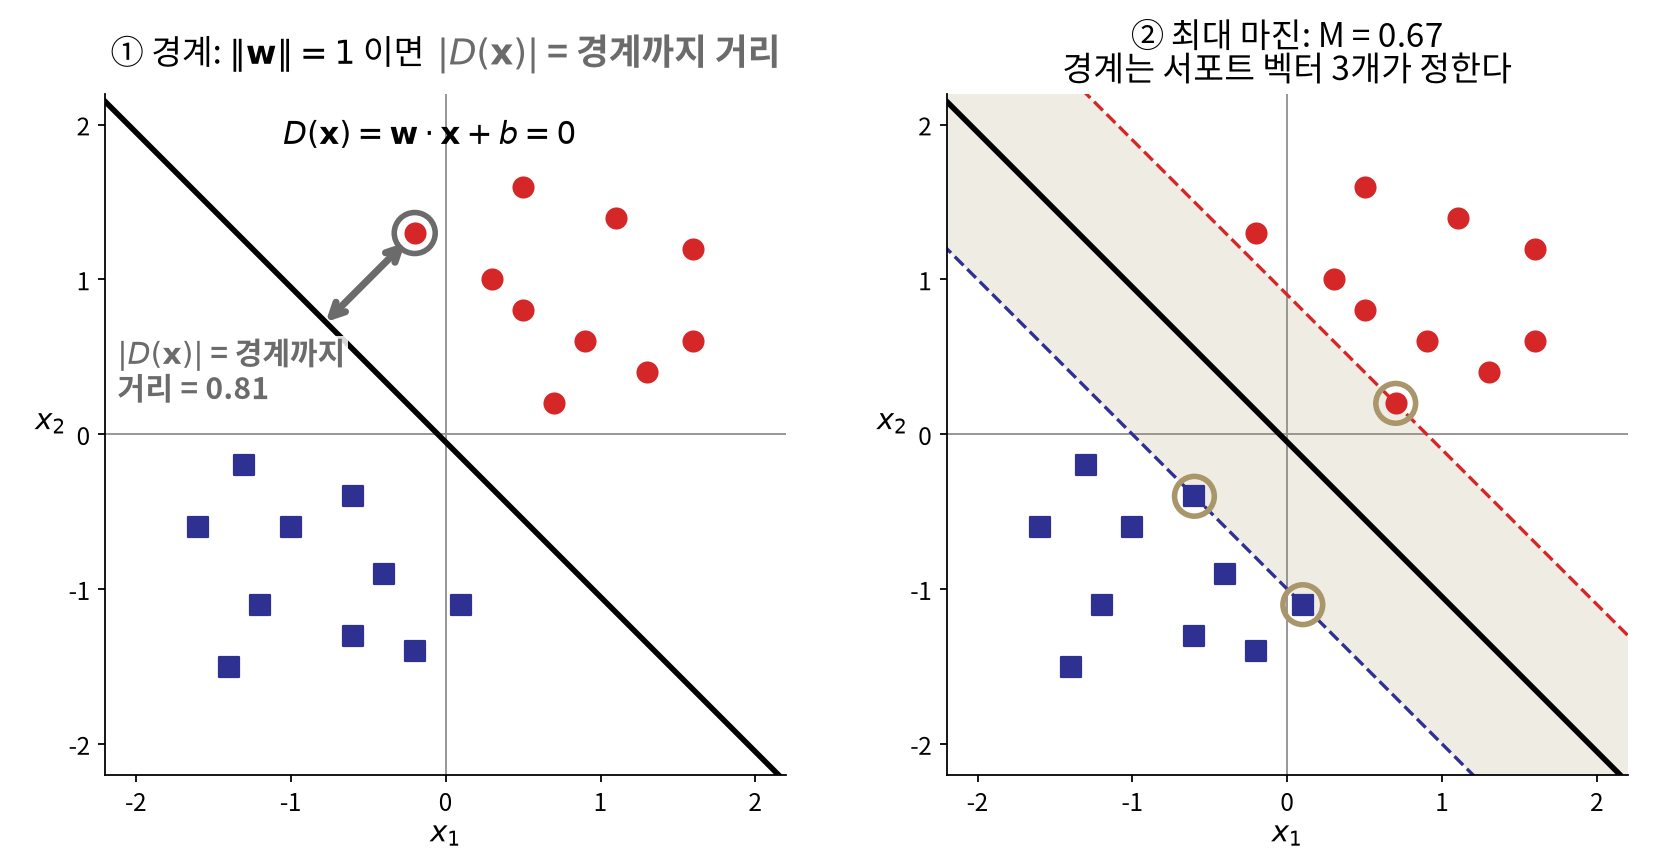
\includegraphics[width=0.8\linewidth]{kn_recap.png}\par\vskip0.2em
\vfill
\note{지난 시간 내용을 그림 두 장으로 정리합니다. 첫 번째 그림, 경계는 초평면 D x, w 점곱 x 더하기 b가 0인 곳이고, w의 길이를 1로 맞추면 D x의 절댓값이 곧 그 점에서 경계까지의 거리입니다. 그림에서 파란 동그라미를 친 빨간 점은 D x가 0.81이고, 경계까지 거리도 0.81입니다. 두 번째 그림, 가장 가까운 거리 M을 최대로 하는 것이 최대 마진이고, 마진은 0.67이고, 경계는 동그라미 친 서포트 벡터 3개가 정합니다.}
\end{frame}

% --- 오늘의 두 질문
\begin{frame}{오늘의 질문}
\vfill
\centering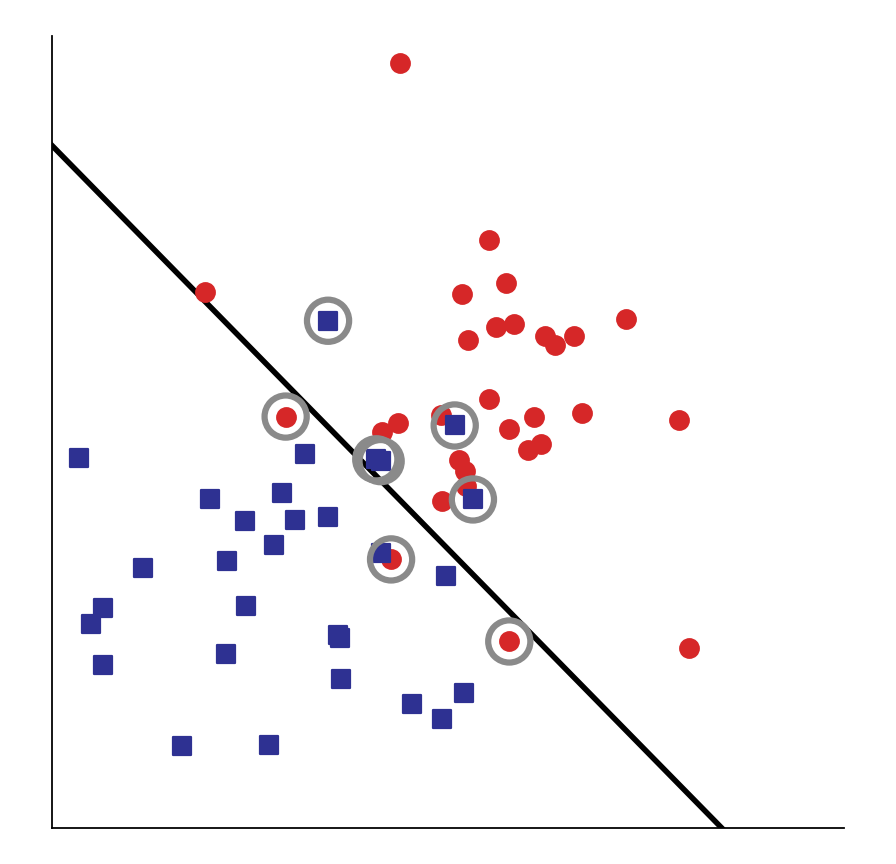
\includegraphics[height=0.7\textheight]{kn_overlap.png}\\[0.4em]
{\Large 두 색이 \kq{섞여 있으면}?}
\vfill
\note{오늘의 질문입니다. 그림처럼 두 색이 경계 근처에서 뒤섞여 있으면 어떻게 할까요. 실제 데이터에는 이런 점이 늘 있습니다. 그러면 어떤 직선을 그어도 몇 점은 반대쪽에 남습니다. 지난 시간의 최대 마진은 모든 점이 제 쪽에 있어야 답이 있었으니, 이런 데이터에서는 답이 없습니다. 먼저 지난 시간 문제를 점마다 당기는 힘 알파를 붙여 푸는 방법으로 배우고, 그다음 몇 점은 넘어가도 되게 하는 소프트 마진으로 이 질문에 답합니다.}
\end{frame}

\section{식 다시 쓰기}
% --- 크기 문제: 같은 선, 숫자는 무한히 많다
\begin{frame}{복습: 같은 선을 쓰는 숫자는 무한히 많다}
\vfill
\centering
{\large $\displaystyle \max_{\mathbf{w},\,b,\ \lVert\mathbf{w}\rVert = 1}\ \min_{k}\ y_k D(\mathbf{x}_k)$ \qquad 왜 $\lVert\mathbf{w}\rVert = 1$ 로 묶었나?}\\[1.1em]
\renewcommand{\arraystretch}{1.45}
{\normalsize\begin{tabular}{l|c|c|c|c}
$\mathbf{w}$, \; $b$ & $\lVert\mathbf{w}\rVert$ & $D(\mathbf{x}_r)$ & 거리 $= D(\mathbf{x}_r)/\lVert\mathbf{w}\rVert$ & 묶은 것\\ \hline
$(0.71,\ 0.71)$, \; $0.04$ & 1 & 0.67 & \kb{0.67} & $\lVert\mathbf{w}\rVert = 1$ (지난 시간)\\
$(1.41,\ 1.41)$, \; $0.07$ \;($\times 2$) & 2 & 1.34 & \kb{0.67} & 없음\\
$(1.05,\ 1.05)$, \; $0.05$ & 1.49 & \kq{1} & \kb{0.67} & $D(\mathbf{x}_r) = 1$ (오늘)
\end{tabular}}\\[1em]
{\large 선도 거리도 \textbf{그대로}, 숫자 크기만 다르다 $\to$ 하나를 고를 \kq{약속}이 필요하다}\\[0.3em]
{\small\color{gray} $\mathbf{x}_r$ = \textbf{가장 가까운} 빨간 점 서포트 벡터 $(0.7,\ 0.2)$}
\vfill
\note{지난 시간 마지막 식은 w의 길이를 1로 묶고, 가장 가까운 점의 거리를 최대로 하는 것이었습니다. 왜 길이를 묶었을까요. 같은 선을 쓰는 방법이 무한히 많기 때문입니다. w와 b에 같은 수를 곱해도 D x가 0인 곳은 그대로라 선이 같습니다. 표를 봅시다. 첫 줄은 지난 시간의 답입니다. 길이가 1이고 빨간 서포트 벡터의 값이 0.67, 거리도 0.67입니다. 둘째 줄은 두 배를 한 것입니다. 길이는 2, 값은 1.34로 두 배가 되지만, 거리는 값을 길이로 나눈 것이라 여전히 0.67입니다. 셋째 줄은 서포트 벡터의 값이 딱 1이 되게 크기를 고른 것입니다. 길이는 1.49이고 거리는 역시 0.67입니다. 세 줄 모두 같은 선입니다. 그래서 무한히 많은 것 중 하나를 고르는 약속이 필요합니다. 지난 시간의 약속은 w의 길이가 1이었습니다. 원 논문은 여기서 약속을 바꿉니다.}
\end{frame}

% --- 복습: 점에서 경계까지 거리 (02-2 의 참고 쪽)
\begin{frame}{복습: 점에서 경계까지 거리 $= |D(\mathbf{x})| / \lVert\mathbf{w}\rVert$}
\vfill
\begin{columns}[c]
\begin{column}{0.40\textwidth}\centering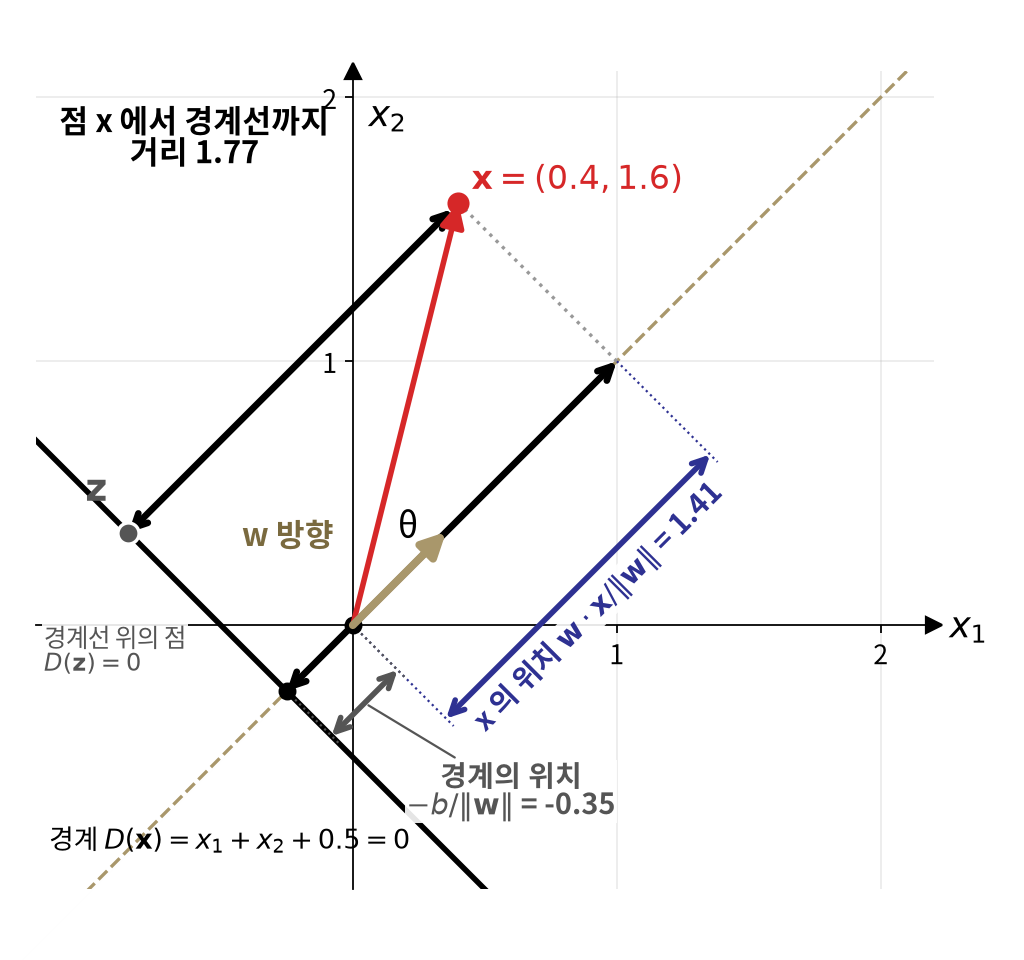
\includegraphics[width=\linewidth]{sv_cos.png}\end{column}
\begin{column}{0.59\textwidth}
{\large \textcolor{fdist}{\textbf{점 $\mathbf{x}$ 에서 경계선까지 거리} $= \dfrac{|D(\mathbf{x})|}{\lVert\mathbf{w}\rVert}$}}\\[0.6em]
\hspace*{2.5em}\fcolorbox{fbeta}{fbeta!8}{\small ※ 두 벡터 사이 각: $\cos\theta = \dfrac{\mathbf{a}\cdot\mathbf{b}}{\lVert\mathbf{a}\rVert\,\lVert\mathbf{b}\rVert}$}\\[0.5em]
{\normalsize \color{fsh}\textbf{1.} $\mathbf{x}$ 의 위치 $\lVert\mathbf{x}\rVert\cos\theta = \tfrac{\mathbf{w}\cdot\mathbf{x}}{\lVert\mathbf{w}\rVert}$}\\[0.4em]
{\normalsize \color{fbd}\textbf{2.} 경계선 위의 점 $\mathbf{z}$ 는 $D(\mathbf{z}) = 0$, 곧 $\mathbf{w}\cdot\mathbf{z} = -b$\\ \hspace*{1.2em}$\to$ 경계의 위치 $= \tfrac{-b}{\lVert\mathbf{w}\rVert}$}\\[0.4em]
{\normalsize \textbf{3.} \textcolor{fdist}{거리} $= \tfrac{\mathbf{w}\cdot\mathbf{x}}{\lVert\mathbf{w}\rVert} - \tfrac{-b}{\lVert\mathbf{w}\rVert} = \tfrac{\mathbf{w}\cdot\mathbf{x} + b}{\lVert\mathbf{w}\rVert} = \tfrac{D(\mathbf{x})}{\lVert\mathbf{w}\rVert}$}\\[0.5em]
{\normalsize 예 $\mathbf{w} = (1, 1)$, $b = 0.5$: \;\textcolor{fsh}{1.41} $-$ (\textcolor{fbd}{$-0.35$}) $=$ \textbf{\textcolor{fdist}{1.77}}}
\end{column}
\end{columns}
\vfill
\note{방금 표에서 거리를 값 나누기 w의 길이로 계산했습니다. 왜 그런지, 지난 시간에 본 거리 공식을 복습합니다. 마진 M은 점에서 경계선까지의 거리입니다. 점과 점 사이가 아니라, 점에서 경계선에 수선을 내린 길이, 그림의 초록 화살표입니다. 이 거리는 D x의 절댓값을 w의 길이로 나눈 것인데, 왜 그런지 코사인으로 세 줄이면 됩니다. 첫째, 두 벡터 사이의 코사인은 점곱을 두 길이로 나눈 것입니다. 양변에 x의 길이를 곱하면, x의 길이 곱하기 코사인 세타, 즉 점 x에서 w 축으로 수선을 내린 발까지의 길이, x의 w 방향 위치가 w 점곱 x 나누기 w의 길이입니다. 그림의 파란 치수선, 1.41입니다. 둘째, 경계는 w에 수직인 직선이라 경계 위의 점은 모두 위치가 같습니다. 경계선 위의 점을 z라고 하면 D z가 0이니 w 점곱 z가 마이너스 b이고, 그래서 경계의 위치는 마이너스 b 나누기 w의 길이입니다. 그림의 회색, 마이너스 0.35입니다. 셋째, 점에서 경계까지의 거리는 두 위치의 차이입니다. 빼면 w 점곱 x 더하기 b를 w의 길이로 나눈 것, 즉 D x 나누기 w의 길이가 됩니다. 반대편 점은 음수가 나오니 절댓값을 씌웁니다. w의 길이가 1일 필요는 없습니다. 나누기 w의 길이는 코사인 식에서 원래 나오는 것입니다. 예는 w가 1, 1이고 b가 0.5, 경계 x1 더하기 x2가 마이너스 0.5인 직선이고, 점은 0.4, 1.6입니다. w의 길이는 루트2, 1.41입니다. 점의 위치는 w 점곱 x 2 나누기 1.41, 1.41이고, 경계의 위치는 마이너스 0.5 나누기 1.41, 마이너스 0.35입니다. 차이는 1.77입니다. D x는 0.4 더하기 1.6 더하기 0.5, 2.5이고, 2.5 나누기 1.41도 1.77로 같습니다. 같은 선을 2 x1 더하기 2 x2 더하기 1로 쓰면 D는 5가 되지만 w의 길이도 2.83이 되어 거리는 똑같이 1.77입니다. D는 식을 몇 배로 쓰느냐에 따라 달라지고, w의 길이로 나누면 그 배율이 사라집니다. w의 길이가 1이면 값이 곧 거리이고, 아니면 w의 길이로 나눠야 거리가 됩니다. 이 공식으로 다음 쪽에서 크기를 정하는 약속을 바꿉니다.}
\end{frame}

% --- M‖w‖ = 1 → M = 1/‖w‖
\begin{frame}{복습: 약속을 $M\lVert\mathbf{w}\rVert = 1$ 로 바꾸면: $M = 1/\lVert\mathbf{w}\rVert$}
\vfill
\centering
\renewcommand{\arraystretch}{1.0}
{\large\begin{tabular}{rl}
\textbf{새 약속} & $M\lVert\mathbf{w}\rVert = 1$ \quad $\to$ \quad \fcolorbox{fbeta}{fbeta!10}{$\displaystyle M = \frac{1}{\lVert\mathbf{w}\rVert}$}\\[1.05em]
\textbf{조건} & 모든 점의 거리가 $M$ 이상: \; $\dfrac{y_k D(\mathbf{x}_k)}{\lVert\mathbf{w}\rVert} \ge M = \dfrac{1}{\lVert\mathbf{w}\rVert}$ \; $\to$ \; \kb{$y_k D(\mathbf{x}_k) \ge 1$}\\[1.05em]
\textbf{목표} & $M$ 최대 \; $=$ \; $\dfrac{1}{\lVert\mathbf{w}\rVert}$ 최대 \; $=$ \; \kb{$\lVert\mathbf{w}\rVert$ 최소}
\end{tabular}}\\[0.8em]
\fcolorbox{fbeta}{fbeta!8}{\large $\displaystyle \min_{\mathbf{w},\,b}\ \tfrac{1}{2}\lVert\mathbf{w}\rVert^2$ \quad 조건: $y_k D(\mathbf{x}_k) \ge 1$, \; $k = 1, \dots, p$}\\[0.35em]
{\small\color{gray} $\tfrac12$ 과 제곱은 미분하기 쉬우라고 (답은 같다)}\\[0.6em]
{\large 풀고 나면 마진 \; $M^* = \dfrac{1}{\lVert\mathbf{w}^*\rVert} = \dfrac{1}{1.49} = \kb{0.67}$}
\vfill
\note{원 논문은 w의 길이를 1로 묶는 대신, 마진 M과 w의 길이의 곱을 1로 묶습니다. 양변을 w의 길이로 나누면 M은 1 나누기 w의 길이입니다. 이것이 오늘의 핵심입니다. 마진이 w의 길이 하나로 정해집니다. 이제 조건을 다시 씁니다. 모든 점은 경계에서 M 이상 떨어져야 합니다. 점의 거리는 y k D x k 나누기 w의 길이이고, M 자리에 1 나누기 w의 길이를 넣으면 양쪽에 같은 분모가 있어서 지워집니다. 남는 것은 y k D x k가 1 이상입니다. 목표도 다시 씁니다. M을 최대로 하는 것은 1 나누기 w의 길이를 최대로 하는 것이고, 분수를 크게 하려면 분모를 작게 해야 하니, w의 길이를 최소로 하는 것입니다. 그래서 아래 상자의 문제가 됩니다. 원 논문은 w 길이 제곱을 최소로 한다고 쓰고, 뒤의 라그랑주 식에서 2분의 1을 붙입니다. 길이가 가장 작은 w는 제곱도 가장 작고 2분의 1을 곱해도 마찬가지라 답은 같습니다. 이 문제를 풀어 w 별을 구하면 마진은 1 나누기 w 별의 길이입니다. 이 데이터에서는 1 나누기 1.49, 0.67입니다. 지난 시간과 똑같은 마진입니다.}
\end{frame}

\section{$\alpha$ 로 학습}
% --- 왜 α 로 쓸 수 있나
\begin{frame}{왜 $\mathbf{w}$ 를 $\alpha$ 로 쓸 수 있나: 점을 더해서 만들었으니까}
\vfill
\centering
{\large 지난 시간의 학습: \; $\mathbf{w} = 0$ 에서 출발, 한 걸음마다 \; $\mathbf{w} \leftarrow \mathbf{w} + \eta\, y_k \mathbf{x}_k$}\\[0.7em]
\renewcommand{\arraystretch}{1.3}
{\large\begin{tabular}{r|l|c}
 & $\mathbf{w}$ 에 일어난 일 (예: $\eta = 0.1$) & $\mathbf{w}$\\ \hline
처음 & 아무것도 안 더함 & $(0,\ 0)$\\
\textcolor{ksared}{빨강 $(0.7, 0.2)$} 가 밂 & $+\,0.1 \times (0.7,\ 0.2)$ & $(0.07,\ 0.02)$\\
\textcolor{ksablue}{파랑 $(-0.6, -0.4)$} 가 밂 & $-\,0.1 \times (-0.6,\ -0.4)$ & $(0.13,\ 0.06)$\\
$\vdots$ & 늘 점의 $y_k \mathbf{x}_k$ 만 더한다 & $\vdots$
\end{tabular}}\\[0.8em]
\fcolorbox{fbeta}{fbeta!10}{\large $\displaystyle \mathbf{w} = \sum_{k} \alpha_k y_k \mathbf{x}_k$ \qquad $\alpha_k$ = 점 $k$ 를 \textbf{더한 양의 합} ($\ge 0$)}\\[0.6em]
{\large 오늘: $\mathbf{w}$ 를 직접 고치지 말고 \kb{$\alpha$ 를 고치자}. 선은 따라 움직인다}
\vfill
\note{왜 w를 점마다의 숫자 알파로 쓸 수 있을까요. 어려운 도구 없이 지난 시간의 학습만 보면 됩니다. w는 0에서 출발했고, 한 걸음마다 한 일은 점 하나의 y x에 학습률을 곱해 더한 것뿐입니다. 예를 들어 학습률 0.1로 빨간 점 0.7, 0.2가 한 번 밀면 w는 0.07, 0.02이고, 이어서 파란 점 마이너스 0.6, 마이너스 0.4가 밀면 파랑은 y가 마이너스 1이라 빼기가 되어 0.13, 0.06이 됩니다. 몇 걸음을 가도 w 안에는 점들의 y x를 더한 것 말고는 아무것도 없습니다. 그러니 점마다 지금까지 더한 양을 모으면 그것이 알파이고, w는 알파 y x의 합입니다. 더하기만 했으니 알파는 0 이상이고, 한 번도 밀지 않은 점은 0입니다. 지난 시간에 w의 길이를 1로 맞춘 것은 양수로 나눈 것이라 이 꼴이 그대로입니다. 오늘은 거꾸로, w를 직접 고치지 않고 알파를 고칩니다. 라그랑주 방법으로 같은 식이 나오는 것은 덱 맨 뒤 Appendix에 있습니다. 원 논문의 식 16입니다.}
\end{frame}

% --- 비유: 못 박힌 판 위의 두 자
\begin{frame}{비유: 못 박힌 판 위에서 벌어지는 두 자}
\vfill
\centering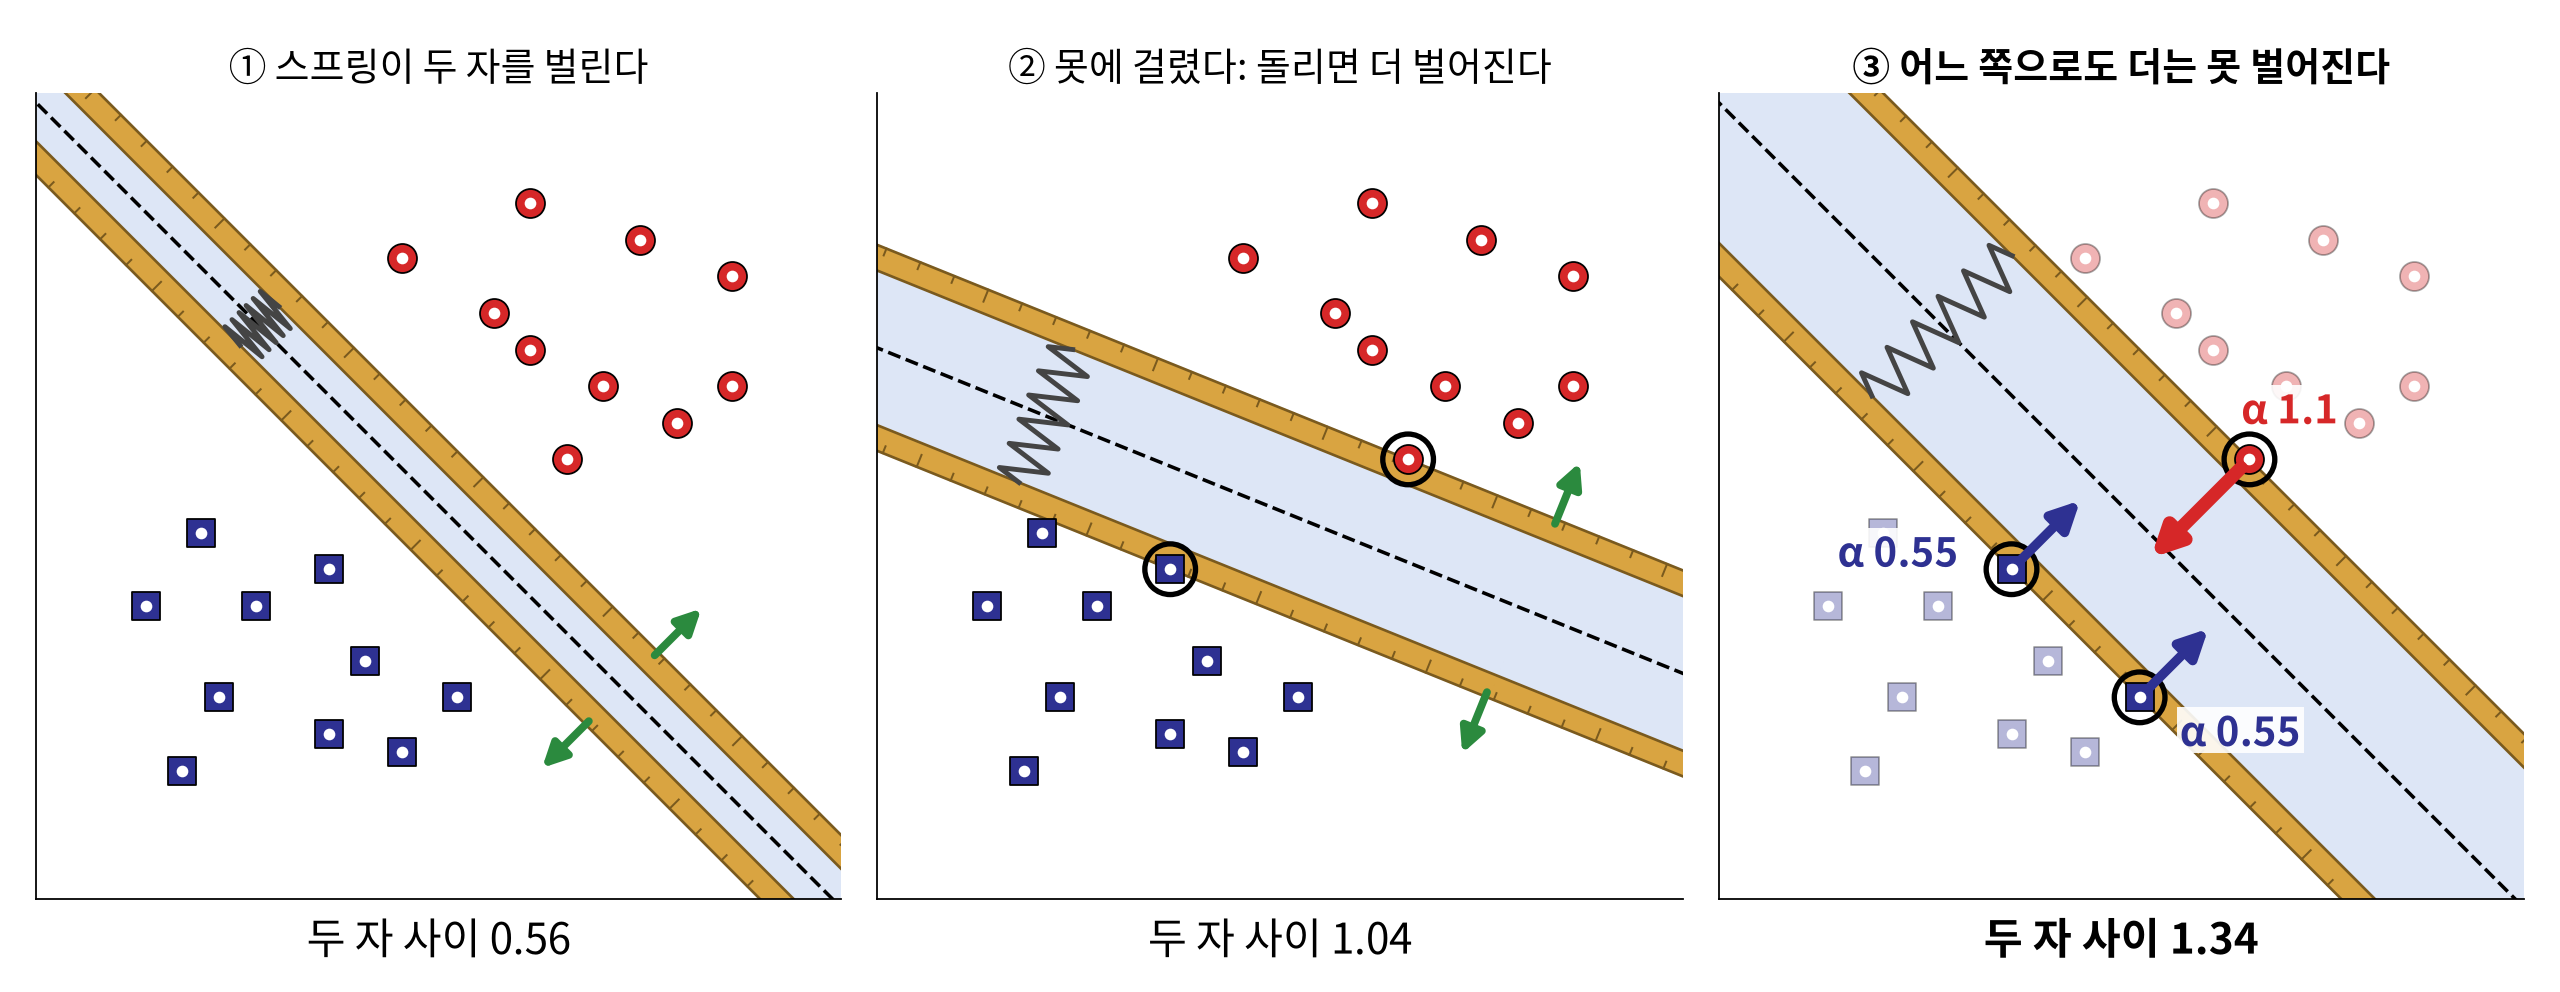
\includegraphics[width=0.84\linewidth]{kn_nails.png}\par\vskip0.2em
{\large 못 = 학습 점 \;·\; 두 자 사이 = 길 폭 $2M$}\\[0.15em]
{\large 자가 닿은 못 = \kb{서포트 벡터}, 못이 당기는 힘 = \kq{$\alpha$} \;·\; 안 닿은 못은 힘 0}
\vfill
\note{SVM을 손에 잡히는 장치로 생각해 봅시다. 나무판에 못이 박혀 있습니다. 못 하나가 학습 점 하나이고, 빨간 못과 파란 못이 있습니다. 못은 움직이지 않습니다. 그 사이에 나란한 자 두 개를 놓고, 가운데의 스프링이 두 자를 서로 밀어냅니다. 두 자는 늘 나란하지만, 함께 돌 수도 있고 함께 미끄러질 수도 있습니다. 첫째 그림, 아직 어느 못에도 닿지 않아서 스프링이 자를 계속 벌립니다. 둘째 그림, 이 각도에서 벌리다 보니 빨간 못 하나와 파란 못 하나에 걸렸습니다. 이 각도에서는 폭 1.04가 끝입니다. 그런데 못이 두 개뿐이라 자가 돌 수 있고, 돌리면 더 벌어집니다. 셋째 그림, 돌리고 미끄러지다가 어느 쪽으로도 더 못 벌어지는 자리에서 멈춥니다. 두 자 사이가 1.34, 길의 폭이고, 한가운데 점선이 SVM의 경계입니다. 이때 못 세 개가 자를 버티고 있습니다. 못은 자가 더 벌어지지 못하게 붙잡고 당깁니다. 이 당기는 힘이 알파입니다. 빨간 못 하나가 1.1, 파란 못 둘이 0.55씩입니다. 양쪽 힘의 합이 같아서 자가 한쪽으로 밀려 가지 않고, 돌림힘도 맞아서 돌지도 않습니다. 자에 닿지 않은 나머지 못은 아무 힘도 주지 않아서, 뽑아 버려도 자는 그대로입니다. 이것이 알파가 0이라는 뜻이고, 서포트 벡터만으로 경계가 정해지는 이유입니다. 교실에서는 자 두 개와 압정 몇 개로 직접 보여 줄 수 있습니다.}
\end{frame}

% --- w = 파랑 중심 → 빨강 중심
\begin{frame}{$\mathbf{w}$ = 파랑 중심에서 빨강 중심으로 가는 화살표}
\vfill
\centering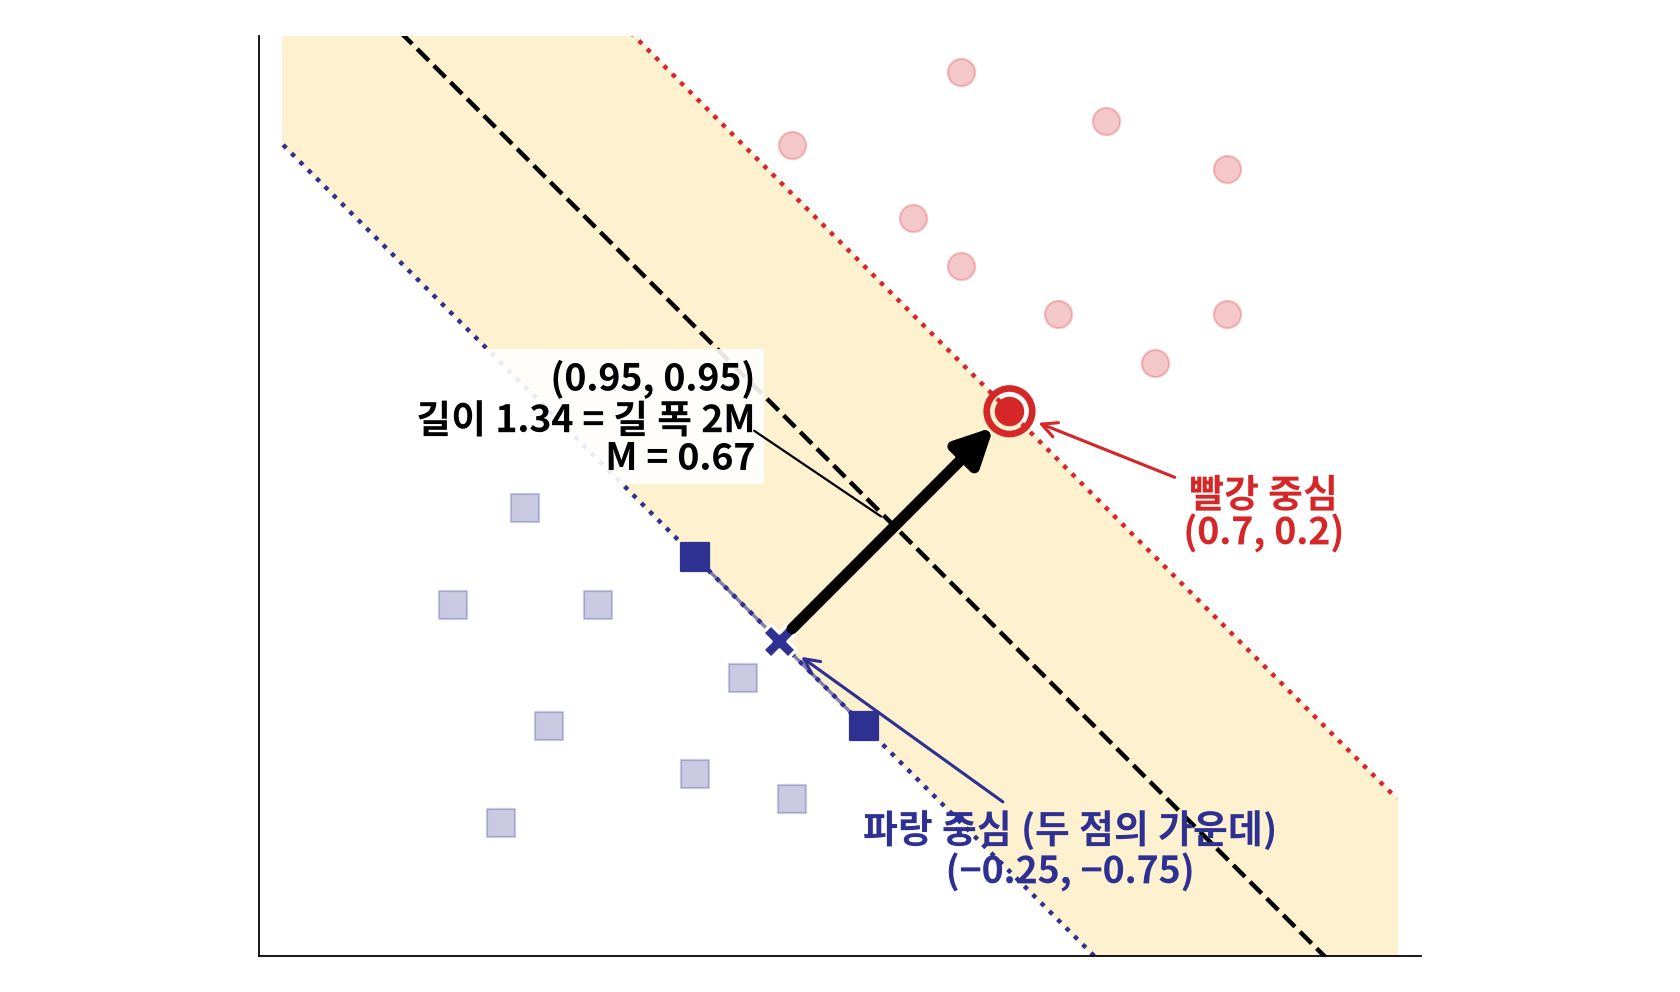
\includegraphics[width=0.60\linewidth]{kn_onearrow.png}\par\vskip0.3em
{\large $\mathbf{w} = S \times (\textcolor{ksared}{\text{빨강 중심}} - \textcolor{ksablue}{\text{파랑 중심}}) = 1.11 \times (0.95,\ 0.95) = (1.05,\ 1.05)$}\\[0.2em]
{\normalsize 중심 = 당기는 힘 $\alpha$ 로 무게를 준 평균 \quad $S$ = 한쪽 힘의 합 (양쪽 같다)}
\vfill
\note{w는 알파 y x를 모두 더한 것이라고 하면 바로 와닿지 않으니, 그림으로 먼저 봅시다. 빨강 점들의 중심과 파랑 점들의 중심을 구합니다. 중심은 당기는 힘 알파를 무게로 준 평균입니다. 힘이 0인 점은 들어가지 않으니 서포트 벡터만 남습니다. 이 데이터에서 빨강은 서포트 벡터가 하나라 그 점 0.7, 0.2가 중심이고, 파랑은 두 점의 힘이 같아서 두 점의 가운데, 마이너스 0.25, 마이너스 0.75입니다. 파랑 중심에서 빨강 중심으로 화살표를 하나 긋습니다. 0.95, 0.95입니다. 여기에 한쪽 힘의 합 1.11을 곱하면 1.05, 1.05, 바로 w입니다. 빨강 힘의 합과 파랑 힘의 합이 같아서 이렇게 하나로 묶입니다. 그림을 보면 경계는 이 화살표의 한가운데를 수직으로 지나고, 화살표의 길이 1.34는 길의 폭과 같습니다. 서포트 벡터가 몇 개든 중심은 길 가장자리 위에 있으니 같은 그림이 됩니다.}
\end{frame}

% --- 이야기 2: 마냥 키우면 길이 좁아진다
\begin{frame}{$\alpha$ 를 마냥 키우면? 길이 좁아진다 $\to$ 값을 치르게 한다}
\vfill
\centering
{\large 길 안의 점을 내보내려면 $\alpha$ 를 키운다}\\[0.2em]
{\large 그런데 $\alpha$ 가 크면 $\mathbf{w}$ 가 커지고 \textbf{마진 $M = 1/\lVert\mathbf{w}\rVert$ 이 줄어든다}}\\[0.7em]
\renewcommand{\arraystretch}{1.35}
{\large\begin{tabular}{c|c|c|c|c}
$\alpha$ (답의 몇 배) & \textbf{얻는 것} $\sum\alpha_k$ & 마진 $M$ & \textbf{치르는 값} $\tfrac12\lVert\mathbf{w}\rVert^2$ & \kq{점수} (빼기)\\ \hline
0.5배 & 1.11 & 1.34 & 0.28 & 0.83\\
\textbf{1배} & \textbf{2.22} & \textbf{0.67} & \textbf{1.11} & \textbf{1.11} (최고)\\
2배 & 4.43 & 0.34 & 4.43 & 0
\end{tabular}}\\[1em]
{\large 점수 $=$ \kb{$\sum_k \alpha_k$} $-$ \kq{$\tfrac12\lVert\mathbf{w}\rVert^2$} \qquad {\normalsize ($\tfrac12\lVert\mathbf{w}\rVert^2 = \tfrac{1}{2M^2}$: 길이 좁을수록 비싸다)}}
\vfill
\note{알파를 고치는데 기준이 필요합니다. 길 안의 점을 밖으로 내보내려면 알파를 키워야 합니다. 그런데 알파를 마냥 키우면 w가 커지고, 마진 1 나누기 w의 길이가 줄어서 길이 좁아집니다. 그래서 알파의 합은 얻는 것으로 치되, 길이 좁아지는 만큼 2분의 1 w 길이 제곱을 값으로 치르게 합니다. 이 값은 2 곱하기 마진 제곱분의 1이라 길이 좁을수록 급하게 비싸집니다. 점 20개의 답을 0.5배, 1배, 2배로 바꿔 보면, 얻는 것은 1.11, 2.22, 4.43으로 비례해서 늘지만 값은 0.28, 1.11, 4.43으로 제곱으로 늘어납니다. 뺀 점수는 0.83, 1.11, 0으로 1배에서 가장 높습니다. 이 점수에 J라는 이름을 붙입니다. 표는 답의 비율을 유지한 채 크기만 바꾼 것이고, 실제 학습은 점마다 알파를 따로 고칩니다. 이 식이 왜 정확히 이 모양인지는 라그랑주 방법으로 유도하며, 덱 맨 뒤 Appendix에 있습니다.}
\end{frame}

% --- J: α 에 매기는 점수
\begin{frame}{$J$: 힘 $\alpha$ 에 매기는 점수. 가장 높은 $\alpha$ 가 답}
\vfill
\centering
{\LARGE $\displaystyle \textcolor{ksared}{J(\boldsymbol{\alpha})} = \sum_{k=1}^{p} \alpha_k - \tfrac12\, \Big\lVert \sum_{k=1}^{p} \alpha_k y_k \mathbf{x}_k \Big\rVert^2$}\\[0.5em]
{\normalsize \textbf{파라미터}: $\alpha_1, \dots, \alpha_p$ \quad (점 $\mathbf{x}_k, y_k$ 는 데이터) \\
\normalsize (둘째 합 $=$ 파랑 $\to$ 빨강 화살표 $\mathbf{w}$)}\\[1.1em]
\renewcommand{\arraystretch}{1.35}
{\large\begin{tabular}{rl}
\textbf{할 일} & $J$ 를 \kb{가장 크게} 하는 $\alpha$ 찾기\\
\textbf{규칙} & $\alpha_k \ge 0$ \; (당기기만 한다)\\
 & $\sum_k \alpha_k y_k = 0$ \; (빨강 힘의 합 $=$ 파랑 힘의 합)
\end{tabular}}\\[1em]
\vfill
\note{이제 학습할 것을 하나로 정리합니다. 못이 당기는 힘 알파에 점수를 매깁니다. 점수 J는 알파를 모두 더한 값에서 2분의 1 w 길이 제곱을 뺀 것입니다. 뒤 항의 길이 안에 있는 것은 못들이 당긴 힘의 합, 알파 y x를 모두 더한 것이고, 이것이 앞에서 본 화살표 w입니다. J에는 알파와 점만 들어갑니다. 할 일은 J를 가장 크게 하는 알파를 찾는 것 하나입니다. 규칙은 두 개입니다. 못은 당기기만 하니 알파는 0 이상이고, 자가 한쪽으로 밀려 가지 않게 빨강 힘의 합과 파랑 힘의 합이 같아야 합니다. 이 식은 지난 시간의 넓은 길 문제를 라그랑주 방법이라는 도구로 바꿔 쓴 것입니다. 어떻게 바꾸는지는 덱 맨 뒤 Appendix에 있고, 원 논문의 식 14에서 17까지입니다. 알파를 먼저 구하면 w는 따라 나옵니다.}
\end{frame}

% --- 같은 문제를 네 번 고쳐 쓰기
\begin{frame}{$J$ 는 새 문제가 아니다: 같은 문제를 네 번 고쳐 쓴 것}
\vfill
\centering
\renewcommand{\arraystretch}{2.3}
{\normalsize\begin{tabular}{rl}
\textbf{\textcircled{1} 목표와 조건} & $\displaystyle\min_{\mathbf{w},\,b}\ \tfrac12\lVert\mathbf{w}\rVert^2$ \qquad 조건 $y_k D(\mathbf{x}_k) - 1 \ge 0$\\
\textbf{\textcircled{2} 식 하나로} & $\displaystyle L = \tfrac12\lVert\mathbf{w}\rVert^2 - \sum_{k=1}^{p} \kq{$\alpha_k$}\,\big[\,y_k D(\mathbf{x}_k) - 1\,\big]$, \qquad \kq{$\alpha_k \ge 0$}\\
\textbf{\textcircled{3} $\mathbf{w}$ 로 미분 $= 0$} & $\displaystyle \mathbf{w}^* = \sum_{k} \alpha_k y_k \mathbf{x}_k$ \qquad \kb{$\leftarrow$ $\mathbf{w}$ 는 작게: 여기서 끝}\\
\textbf{\textcircled{4} 다시 넣기} & $\displaystyle J = \sum_{k} \alpha_k - \tfrac12\Big\lVert \sum_{k} \alpha_k y_k \mathbf{x}_k \Big\rVert^2$ \qquad \quad \kq{$\leftarrow$ $\alpha$ 는 크게: 학습}
\end{tabular}}\\[0.8em]
{\large 컴퓨터가 하는 일은 \kq{$J$ 를 키우는 것} 하나}\\[0.2em]
{\small 새 생각은 \textcircled{2} 하나: 조건마다 $\alpha_k$ 를 붙여 식 하나로 (라그랑주) \quad \textcircled{4} 는 $\sum_k \alpha_k y_k = 0$ 일 때}
\vfill
\note{J가 갑자기 생긴 새 문제처럼 보일 수 있지만, 처음의 넓은 길 문제를 네 번 고쳐 쓴 것입니다. 첫째, 원래 문제입니다. 2분의 1 w 길이 제곱을 가장 작게 하되 모든 점에서 y D 빼기 1이 0 이상이어야 합니다. 원 논문 식 13이고, 2분의 1은 미분하기 편하라고 붙인 것이라 답은 같습니다. 둘째, 목표에서 조건 곱하기 알파를 빼서 식 하나로 만듭니다. 알파는 0 이상입니다. 식 14, 라그랑주 함수입니다. 여기서 새 생각은 이것 하나입니다. 셋째, 이 식을 w로 미분해 0으로 두면 w는 알파 y x의 합입니다. 식 16이고, 앞에서 점을 더해서 w를 만들었던 것과 같은 꼴입니다. 넷째, 그 w를 다시 식에 넣으면 w가 사라지고 알파만 남는 J가 됩니다. 식 17인데, 알파 y의 합이 0이면 b가 든 항이 사라져 이 간단한 꼴이 됩니다. 방향을 정리하면, w와 b는 L을 작게, 알파는 크게 합니다. w를 작게 하는 일은 셋째 줄에서 미분으로 끝났고, 남은 일은 J, 즉 알파 쪽을 키우는 것 하나입니다. 알파를 키우는 이유는 규칙을 어긴 점에 벌을 주기 위해서입니다. 첫째 줄은 w를 찾는 문제이고, 넷째 줄은 알파를 찾는 문제이며, 답은 같습니다.}
\end{frame}

% --- J 를 키우는 학습 한 걸음
\begin{frame}{$J$ 를 키우는 학습 한 걸음: 값이 1 보다 작으면 더 세게}
\vfill
\centering
{\large 점마다 \textbf{값} $y_k D(\mathbf{x}_k)$ 를 잰다 \qquad $D(\mathbf{x}) = \mathbf{w}\cdot\mathbf{x} + b$}\\[0.9em]
\renewcommand{\arraystretch}{1.3}
{\large\begin{tabular}{rl}
처음 & $\alpha_k = 1/(\text{같은 색 점 수}) = 0.1$, \; $b = 0$\\
\textbf{1.} 힘 & $\alpha_k \leftarrow \max\big(0,\ \alpha_k + \eta\,\textcolor{fgap}{(1 - y_k D(\mathbf{x}_k))}\big)$ \quad (모든 점)\\
\textbf{2.} $b$ & $b \leftarrow b + \eta \sum_{k} \alpha_k y_k$ \quad (양쪽 힘이 안 맞으면 경계가 밀린다)
\end{tabular}}\\[0.8em]
\fcolorbox{fbeta}{fbeta!10}{\begin{minipage}{0.86\linewidth}\centering
{\large \textcolor{fgap}{$1 - y_k D(\mathbf{x}_k)$} = 가장자리(값 $1$)까지 \textbf{모자란 양}}\\[0.2em]
{\normalsize \textbf{음수} $=$ \textbf{마진 밖}의 점 (값 $> 1$, 남는 양) $\to$ $\alpha$ 가 줄어든다}\\[0.3em]
{\small 값 $0.4$ (마진 안): $+0.6$ \kq{더 세게} \quad 값 $1.5$ (마진 밖): $-0.5$ \kb{약하게} \quad 값 $1$ (닿음): $0$ 그대로}
\end{minipage}}\\[0.5em]
{\small 학습률 $\eta = 0.05$ \quad $\alpha_k$ 는 $0$ 아래로 안 내려간다}
\vfill
\note{처음 알파는 같은 색 점의 수 분의 1, 여기서는 빨강과 파랑이 10개씩이라 모두 0.1로 둡니다. 그러면 w는 빨강 평균 빼기 파랑 평균이고, 두 색의 힘의 합이 같습니다. 점이 많으면 J의 꼭대기를 한 번에 못 구하니, J가 커지는 쪽으로 알파를 조금씩 움직입니다. 어느 쪽인지는 점의 값만 보면 됩니다. 값은 라벨 곱하기 D x, 1이면 길 가장자리입니다. J를 알파 k로 미분하면 놀랍게도 1 빼기 이 값입니다. 점 k의 값이 1에서 얼마나 모자라는지입니다. 그래서 한 걸음은 두 줄입니다. 첫째, 모든 점의 알파에 학습률 곱하기 1 빼기 값을 더합니다. 값이 1보다 작은 점, 길 안에 있거나 틀린 점은 알파가 커져서 더 세게 밉니다. 값이 1보다 큰 여유 있는 점은 알파가 줄고, 0 아래로는 못 가게 0에서 막습니다. 값이 딱 1인 점은 그대로입니다. 1 빼기 값이 음수가 되는 점이 바로 마진 밖의 점입니다. 모자란 양이 음수라는 것은 남는다는 뜻입니다. 그래서 끝에는 알파와 여유 중 하나가 0이 됩니다. 둘째, b는 알파 y의 합만큼 움직입니다. 빨강 쪽 힘과 파랑 쪽 힘이 안 맞으면 경계가 밀려 가고, 맞으면, 즉 합이 0이면 멈춥니다. 지난 시간처럼 w의 길이를 맞추는 단계는 없습니다. 처음부터 길 가장자리의 값을 1로 두는 기준이기 때문입니다. J는 원 논문의 식 그대로이지만, 이렇게 조금씩 올라가는 방법은 수업에서 이해하기 쉽게 고른 것입니다. 원 논문은 일반 최적화 프로그램, Powell의 알고리즘을 썼습니다.}
\end{frame}

% --- J 학습을 숫자로
\begin{frame}{$J$ 학습을 숫자로: 지난 시간 점 20개}
\vfill
\centering
\renewcommand{\arraystretch}{1.2}
{\large\begin{tabular}{r|ccc|c|c|c}
걸음 뒤 & \textcolor{ksared}{$\alpha_r$} & \textcolor{ksablue}{$\alpha_{b_1}$} & \textcolor{ksablue}{$\alpha_{b_2}$} & $\alpha > 0$ 인 점 & $\mathbf{w} = \sum \alpha_k y_k \mathbf{x}_k$ & $b$\\ \hline
0 & 0.10 & 0.10 & 0.10 & 20개 & $(1.65,\ 1.82)$ & 0.00\\
1 & 0.07 & 0.06 & 0.06 & 12개 & $(0.19,\ 0.30)$ & 0.00\\
10 & 0.29 & 0.24 & 0.18 & 11개 & $(0.63,\ 0.85)$ & 0.01\\
50 & 0.87 & 0.61 & 0.36 & 4개 & $(0.92,\ 0.95)$ & 0.01\\
100 & 1.09 & 0.60 & 0.46 & \kb{3개} & $(1.08,\ 0.97)$ & 0.00\\
500 & 1.11 & 0.55 & 0.55 & 3개 & $(1.05,\ 1.05)$ & 0.05\\
\hline
sklearn 답 & 1.11 & 0.55 & 0.55 & 3개 & $(1.05,\ 1.05)$ & 0.05
\end{tabular}}\\[0.7em]
{\normalsize 0걸음: $\alpha_k = \tfrac1{10}$ \;$\to$\; $\mathbf{w}$ = \textcolor{ksared}{빨강 평균} $-$ \textcolor{ksablue}{파랑 평균} $= (1.65,\ 1.82)$ = \kb{중심 화살표}}\\[0.2em]
{\small $r = (0.7, 0.2)$, \;$b_1 = (-0.6, -0.4)$, \;$b_2 = (0.1, -1.1)$}
\vfill
\note{지난 시간의 점 20개로 실제로 돌린 숫자입니다. 처음에는 알파를 모두 0.1, b를 0으로 둡니다. 그러면 w는 빨강 평균에서 파랑 평균을 뺀 1.65, 1.82입니다. 파랑 중심에서 빨강 중심으로 가는 화살표이고, 지난 시간의 평균 선과 방향이 같습니다. 이때 길 반폭은 0.41로 좁아서 모든 점이 마진 밖입니다. 그래서 첫 걸음에는 알파가 크게 줄어 12개만 남고, w는 0.19, 0.30으로 작아져 길이 확 넓어집니다. 걸음을 반복하면 알파가 0보다 큰 점이 10걸음에 11개, 50걸음에 4개, 100걸음에 3개입니다. 500걸음이면 알파가 1.11, 0.55, 0.55, w가 1.05, 1.05, b가 0.05로 sklearn의 답과 같습니다. 덱의 다른 쪽에서 빨강 알파를 1.1로 쓰는 것은 파랑 두 개 0.55를 더한 값으로 맞춰 쓴 것이고, 정확한 값은 1.108입니다.}
\end{frame}

% --- 실제 학습: 자가 왔다 갔다 (1/3)
\begin{frame}{두 자가 왔다 갔다 하며 자리를 잡는다 (1/3)}
\vfill
\centering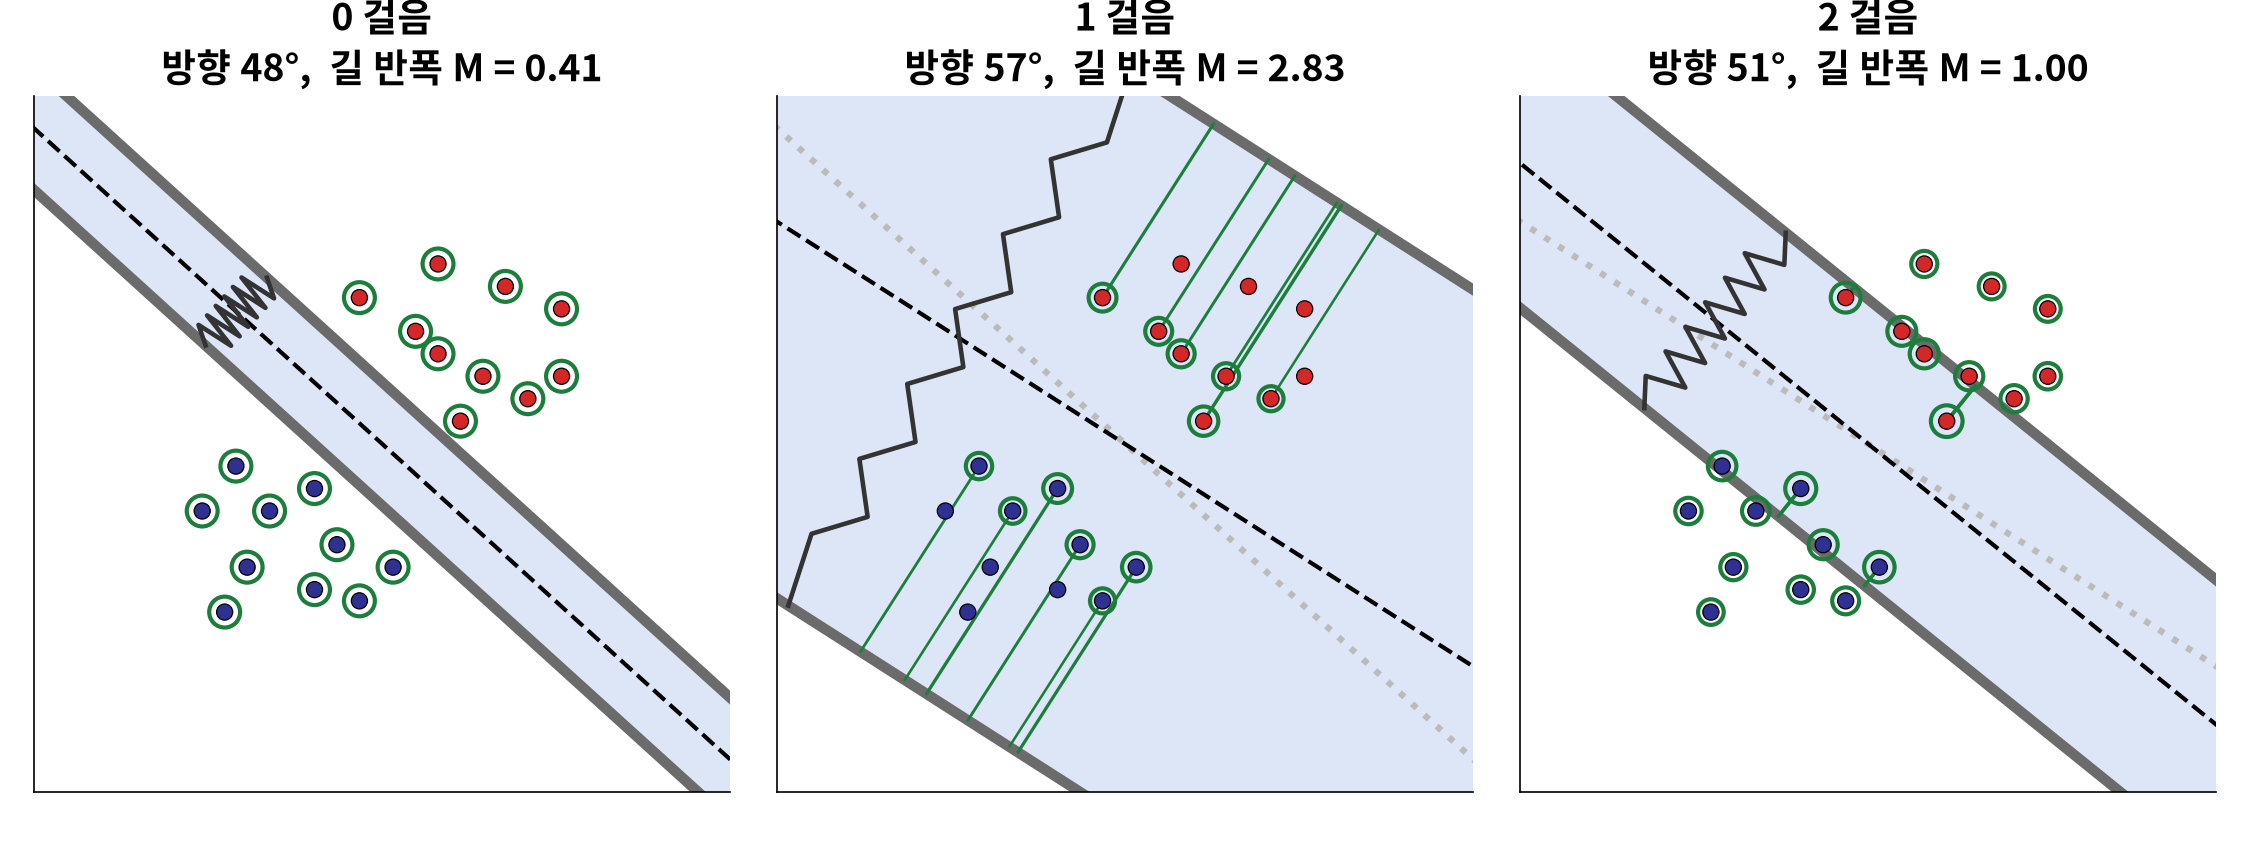
\includegraphics[width=0.93\linewidth]{kn_rock9_1.png}\par\vskip0.3em
{\large 좁은 첫 길 ($M$ 0.41) $\to$ \textbf{확 벌어졌다} (2.83) $\to$ 다시 당긴다 (1.00)}\\[0.2em]
{\normalsize \textbf{스프링}은 벌리고, 길 안(파란 칠)의 점은 \textcolor{fgap}{\textbf{고무줄}}로 당긴다 \quad 굵기 · 고리 $= \alpha$}
\vfill
\note{점 20개를 실제로 학습한 모습입니다. 회색 두 자가 길의 가장자리이고, 파랗게 칠한 곳이 길 안입니다. 가운데 스프링은 두 자를 벌리려 합니다. 길 안에 들어온 점은 자기 쪽 자에 초록 고무줄을 걸어 당기고, 고무줄이 굵고 초록 고리가 클수록 알파가 큽니다. 0걸음에는 알파가 모두 0.1입니다. 선은 두 색의 평균을 가르는 선이고, 길 반폭이 0.41로 좁아 모든 점이 길 밖입니다. 당길 이유가 없으니 첫 걸음에 알파가 확 줄고, 스프링이 이겨서 길이 2.83으로 벌어집니다. 방향은 57도입니다. 이번에는 모든 점이 길 안이라 다시 당겨서, 두 번째 걸음에는 51도, 길 반폭 1.00이 됩니다.}
\end{frame}

% --- 실제 학습: 자가 왔다 갔다 (2/3)
\begin{frame}{두 자가 왔다 갔다 하며 자리를 잡는다 (2/3)}
\vfill
\centering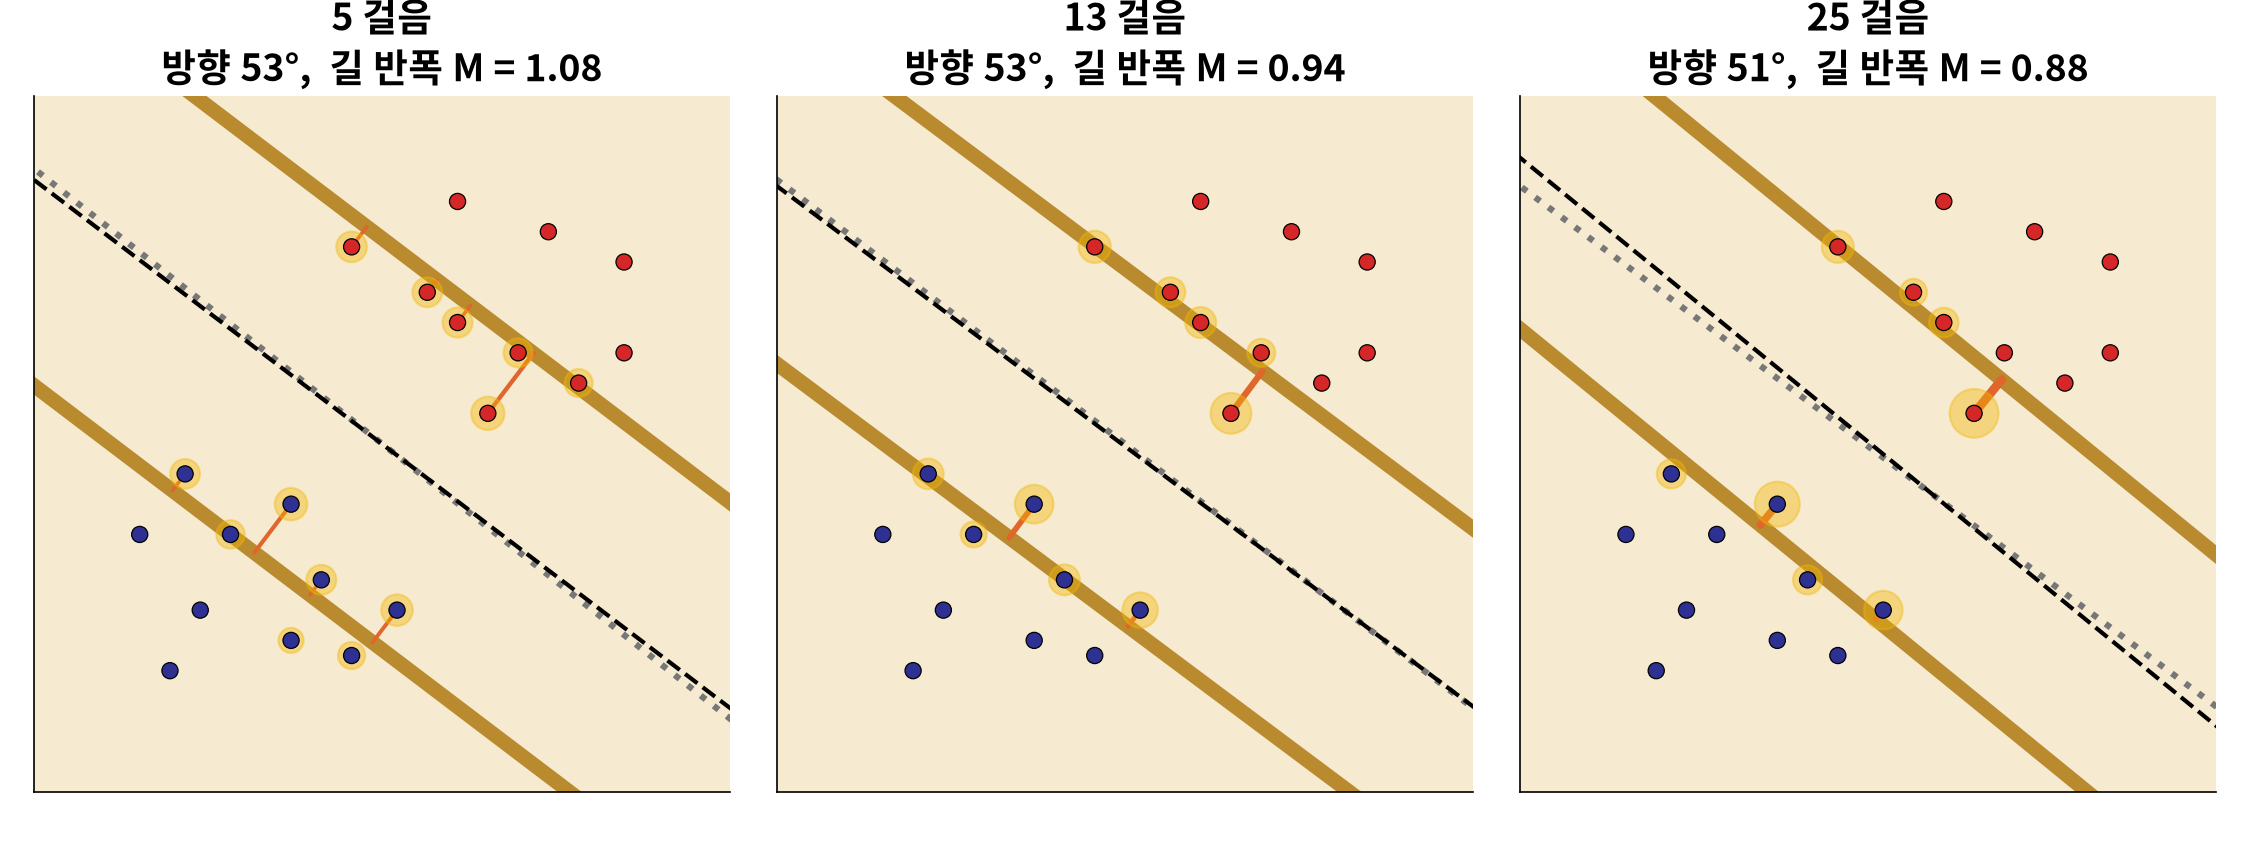
\includegraphics[width=0.93\linewidth]{kn_rock9_2.png}\par\vskip0.3em
{\large 방향 $53^\circ$ 근처에서 길이 \textbf{천천히 좁아진다}}\\[0.2em]
{\normalsize \textbf{스프링}은 벌리고, 길 안(파란 칠)의 점은 \textcolor{fgap}{\textbf{고무줄}}로 당긴다 \quad 굵기 · 고리 $= \alpha$}
\vfill
\note{3걸음에는 54도, 1.32로 한 번 더 출렁입니다. 그 뒤로는 크게 튀지 않습니다. 13걸음에 53도, 0.92, 25걸음에 51도, 0.87입니다. 당기는 점이 점점 줄고 고무줄도 짧아집니다. 회색 점선은 앞 장면의 경계라, 선이 얼마나 움직였는지 볼 수 있습니다.}
\end{frame}

% --- 실제 학습: 자가 왔다 갔다 (3/3)
\begin{frame}{두 자가 왔다 갔다 하며 자리를 잡는다 (3/3)}
\vfill
\centering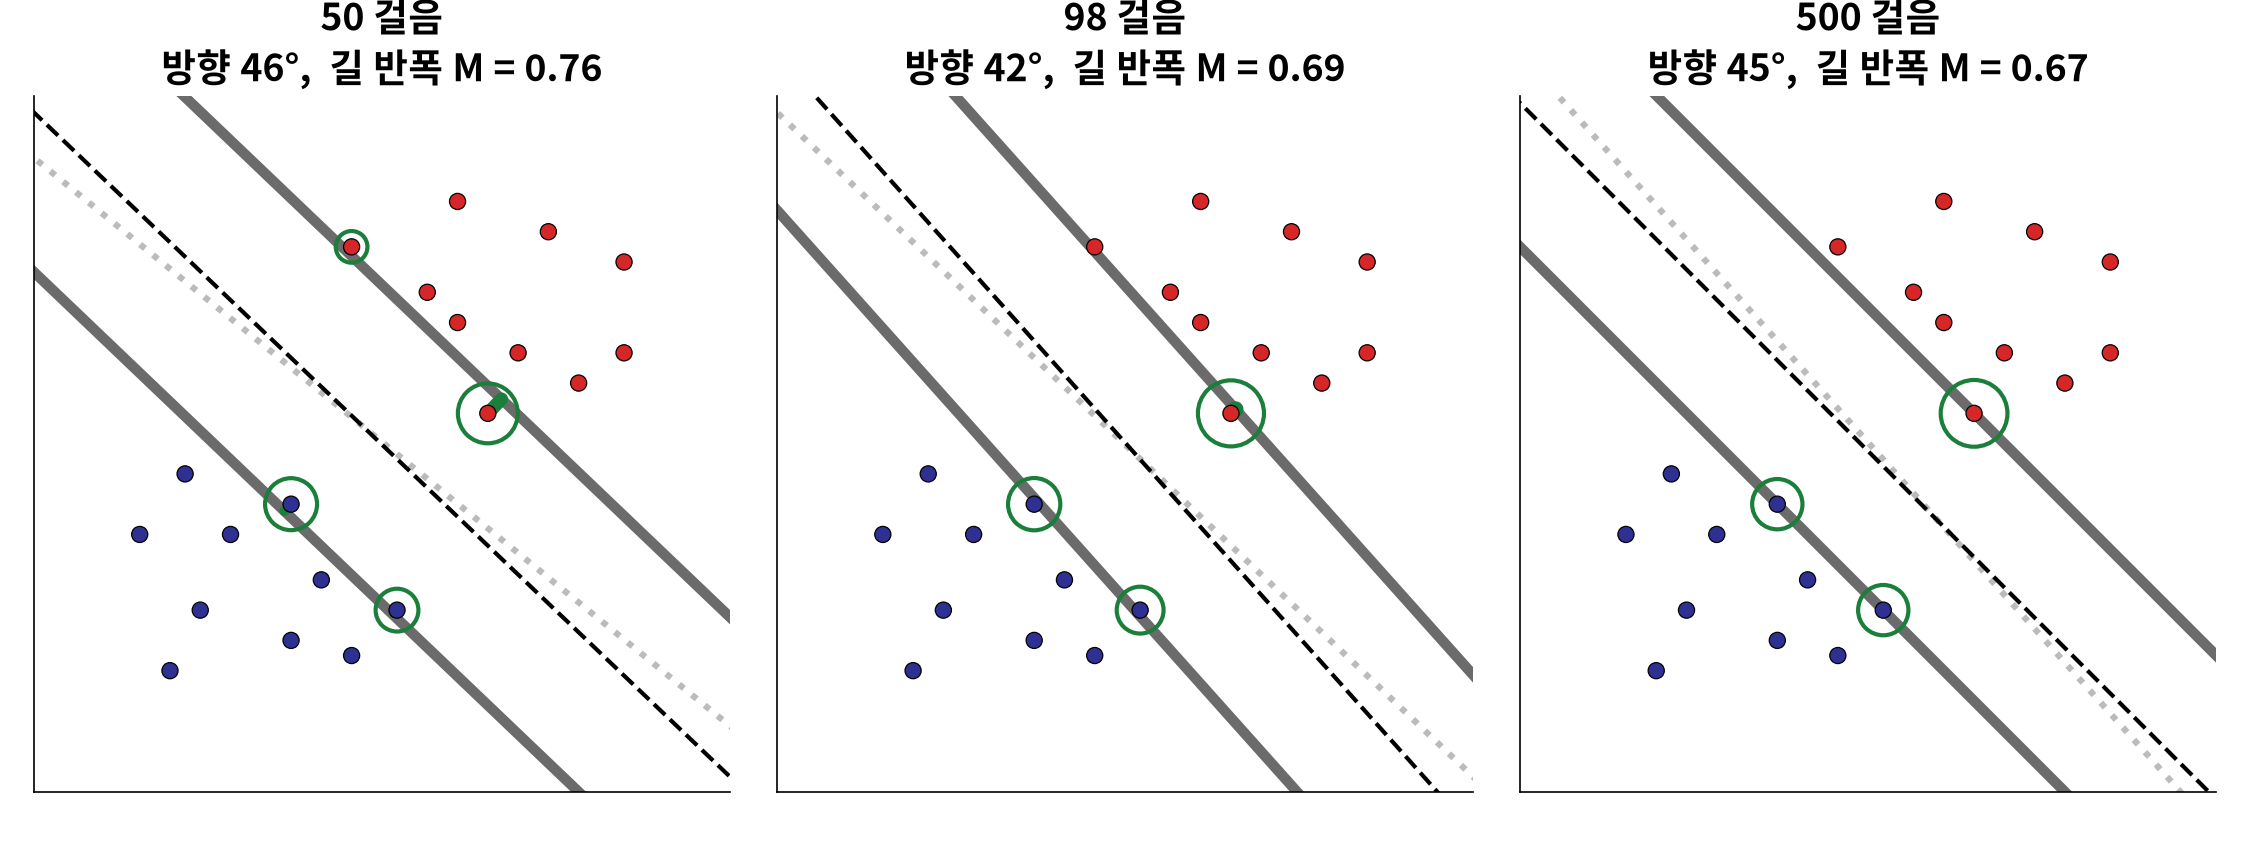
\includegraphics[width=0.93\linewidth]{kn_rock9_3.png}\par\vskip0.3em
{\large 답 $45^\circ$ 를 \kq{지나쳤다가} ($42^\circ$) \kb{돌아와} 멈춘다}\\[0.2em]
{\normalsize \textbf{스프링}은 벌리고, 길 안(파란 칠)의 점은 \textcolor{fgap}{\textbf{고무줄}}로 당긴다 \quad 굵기 · 고리 $= \alpha$}
\vfill
\note{50걸음에는 46도, 0.75입니다. 그런데 자는 답에서 멈추지 않고 계속 돌아 98걸음에는 42도로 지나칩니다. 500걸음에 45도, 길 반폭 0.67에서 멈춥니다. 남은 힘은 자에 닿은 점 3개뿐입니다. 한 번에 답으로 가는 것이 아니라 넘쳤다가 돌아오면서 힘의 균형을 찾습니다. 학습률은 0.05이고, 너무 크게 잡으면 길이 닫혔다 열렸다를 반복하며 멈추지 못합니다.}
\end{frame}

% --- 학습 과정 (클릭해서 넘김)
\begin{frame}{$\alpha$ 를 학습하면: 선이 자리를 잡는 과정}
\vfill
\centering
\only<1>{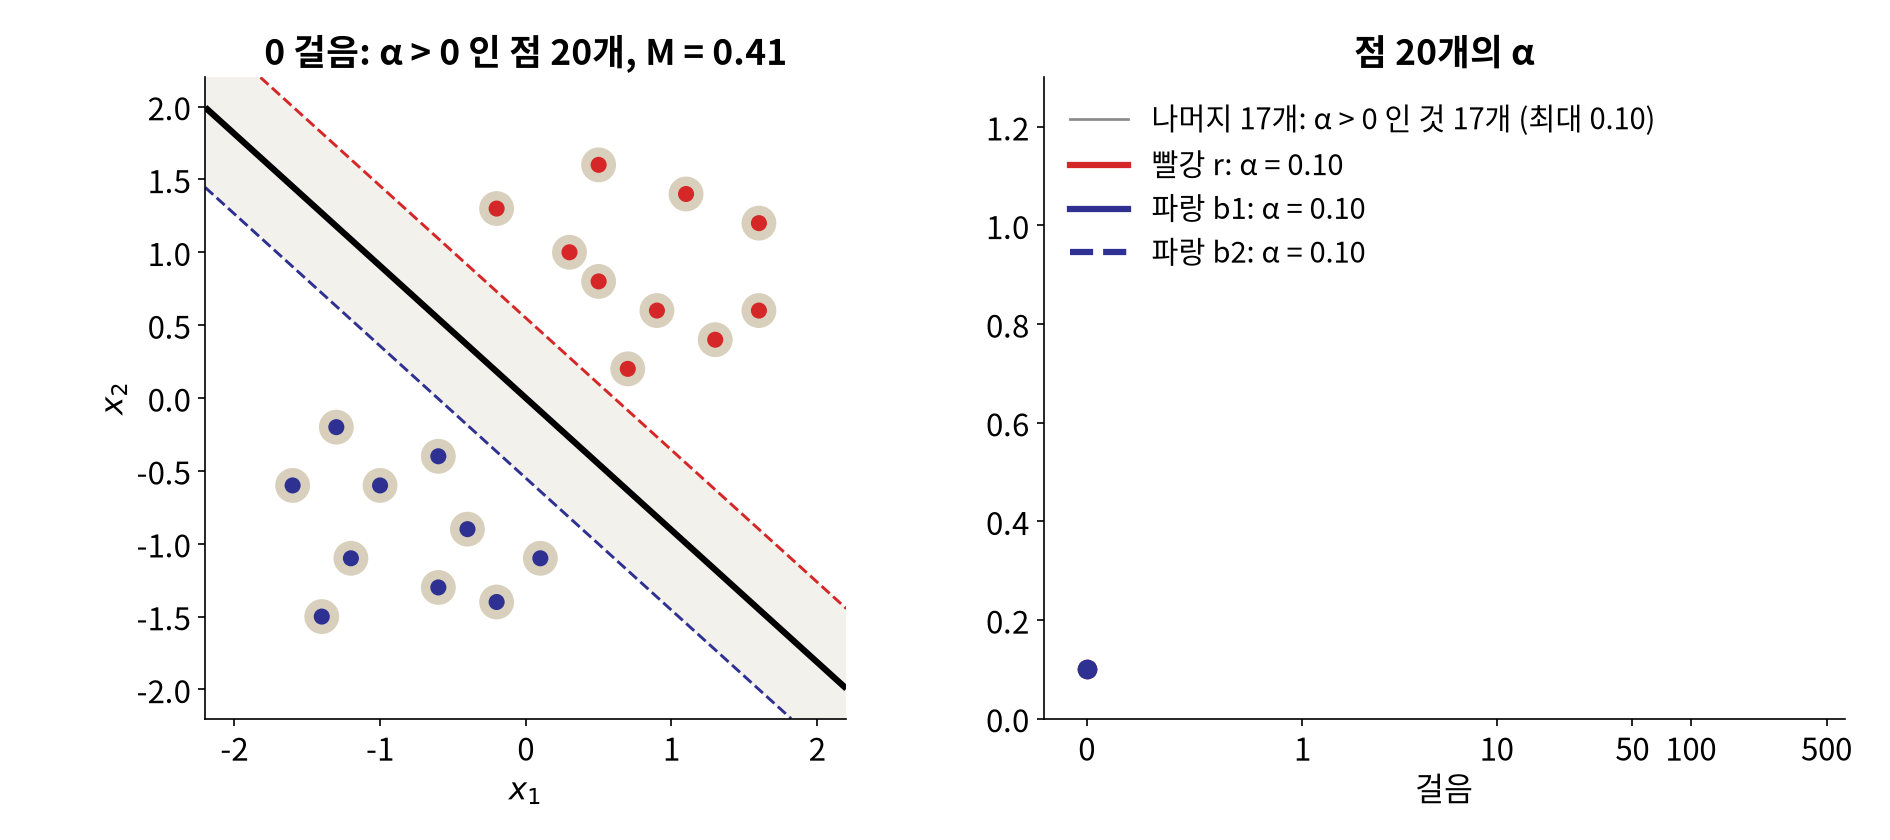
\includegraphics[width=0.88\linewidth]{kn_learn1.png}}%
\only<2>{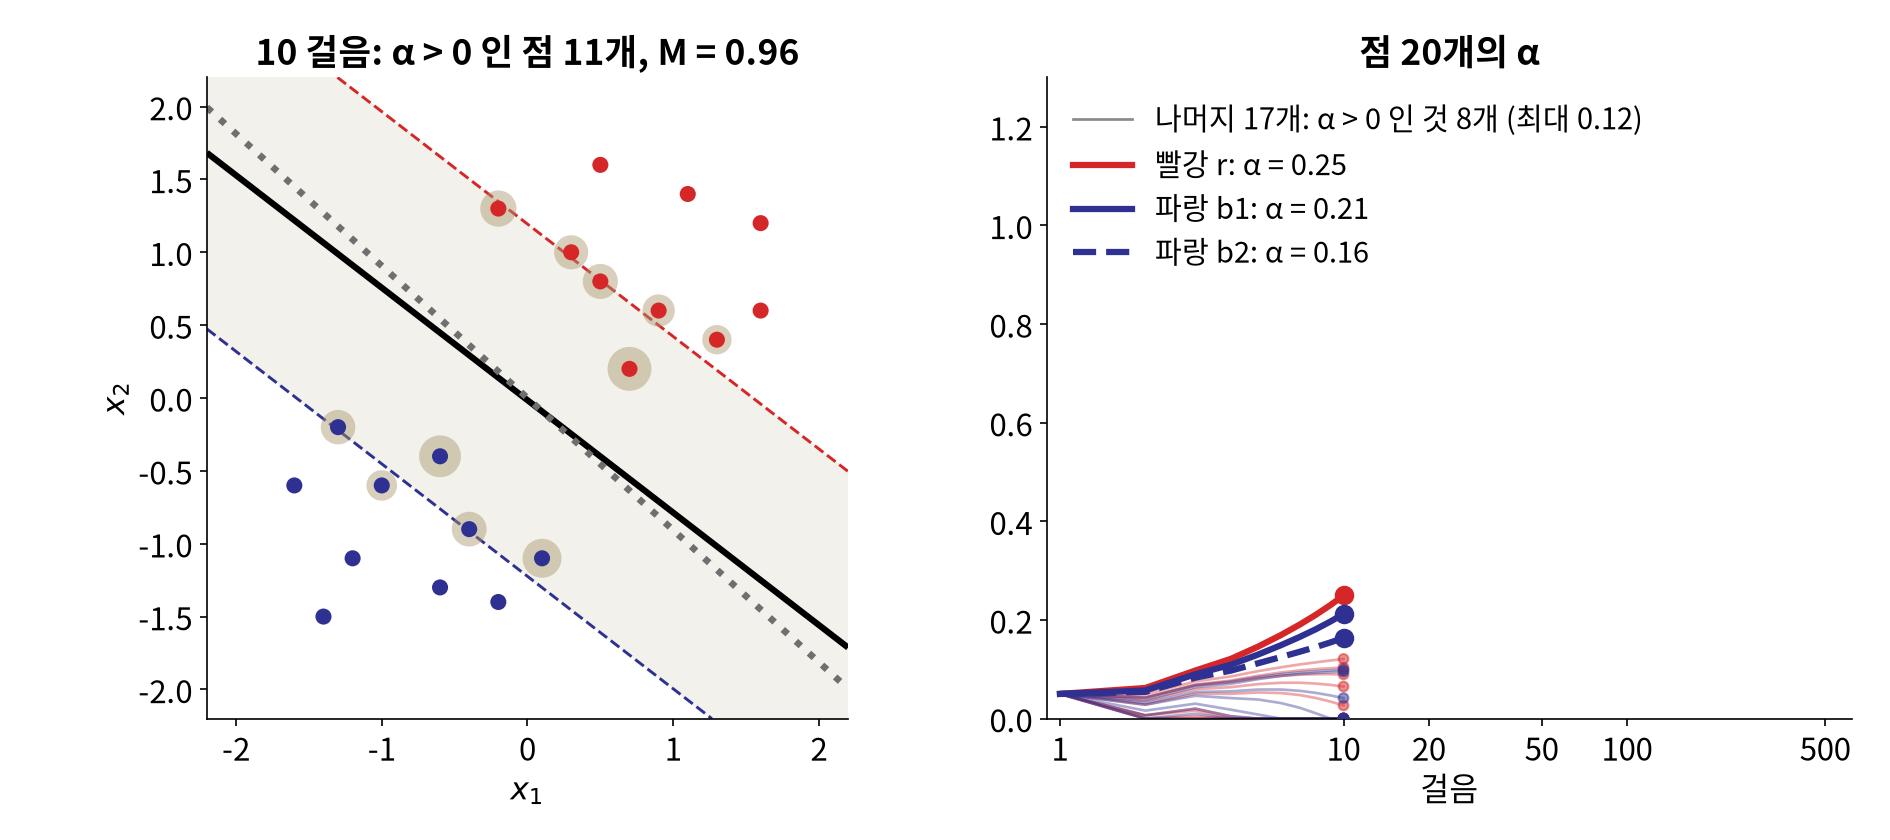
\includegraphics[width=0.88\linewidth]{kn_learn2.png}}%
\only<3>{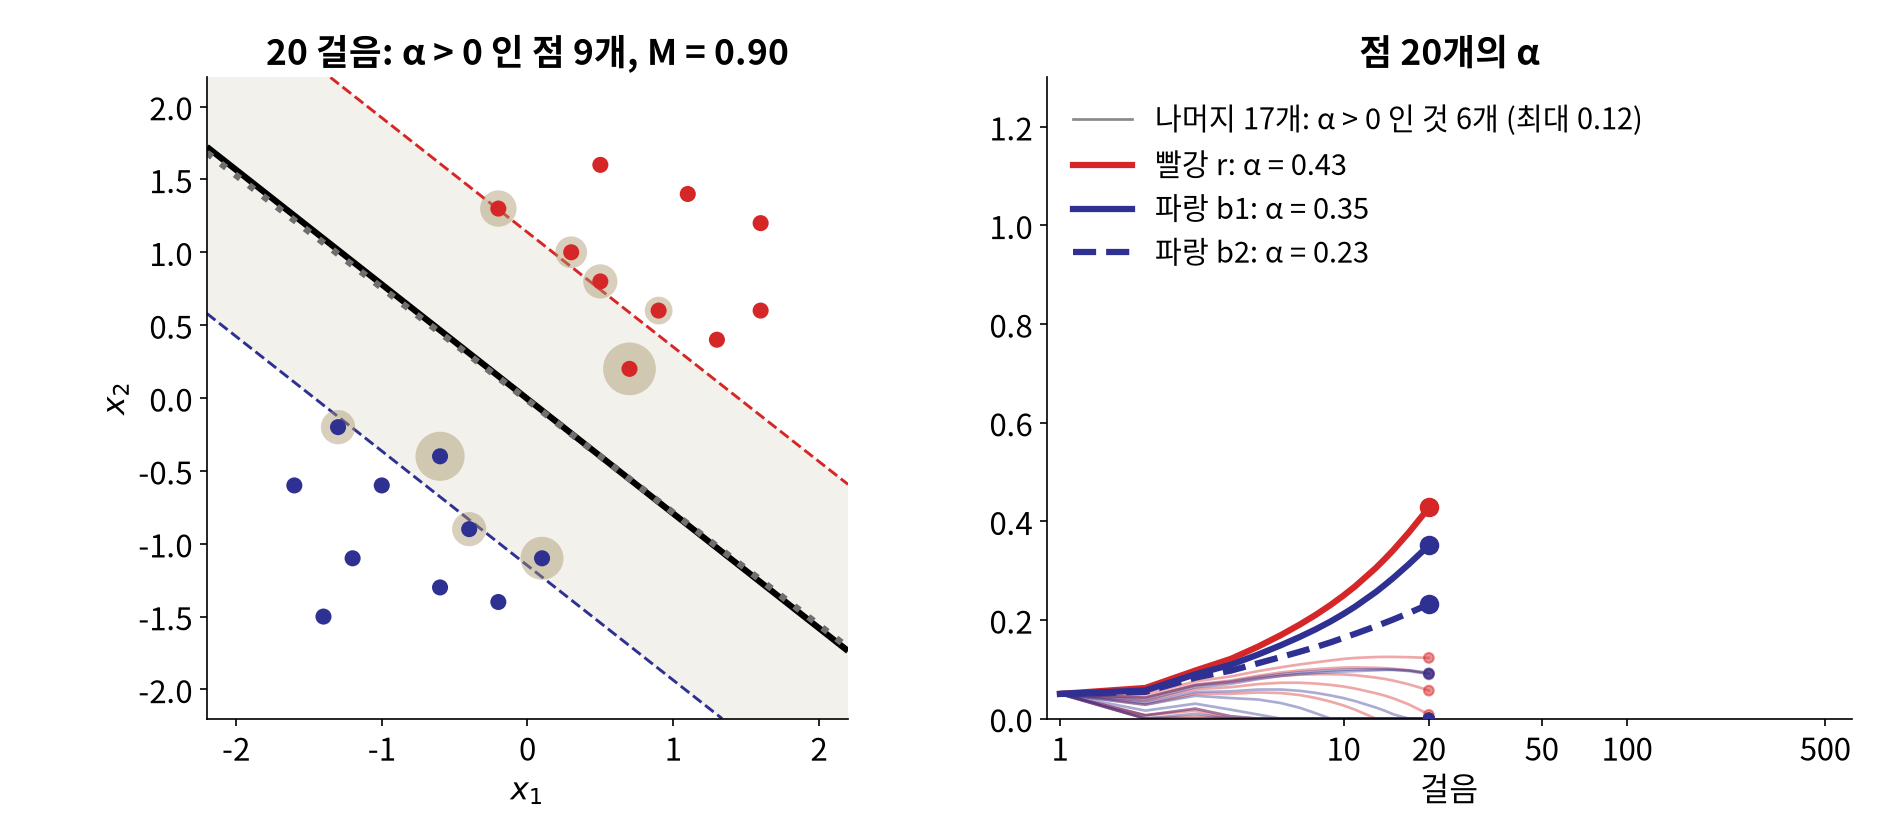
\includegraphics[width=0.88\linewidth]{kn_learn3.png}}%
\only<4>{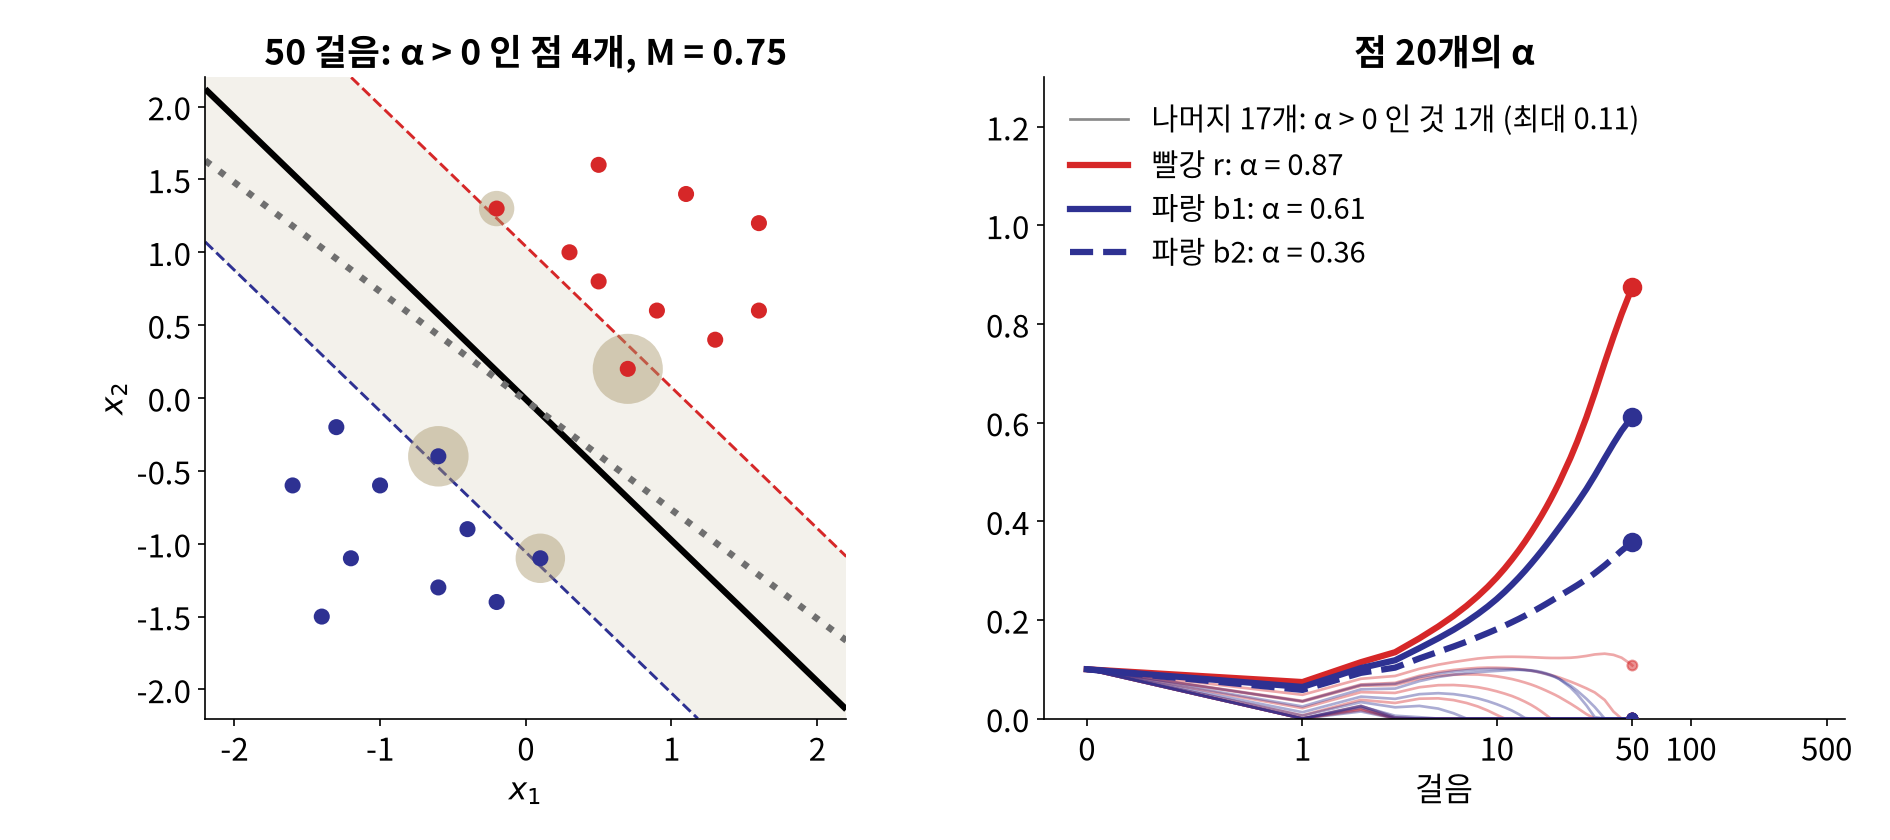
\includegraphics[width=0.88\linewidth]{kn_learn4.png}}%
\only<5>{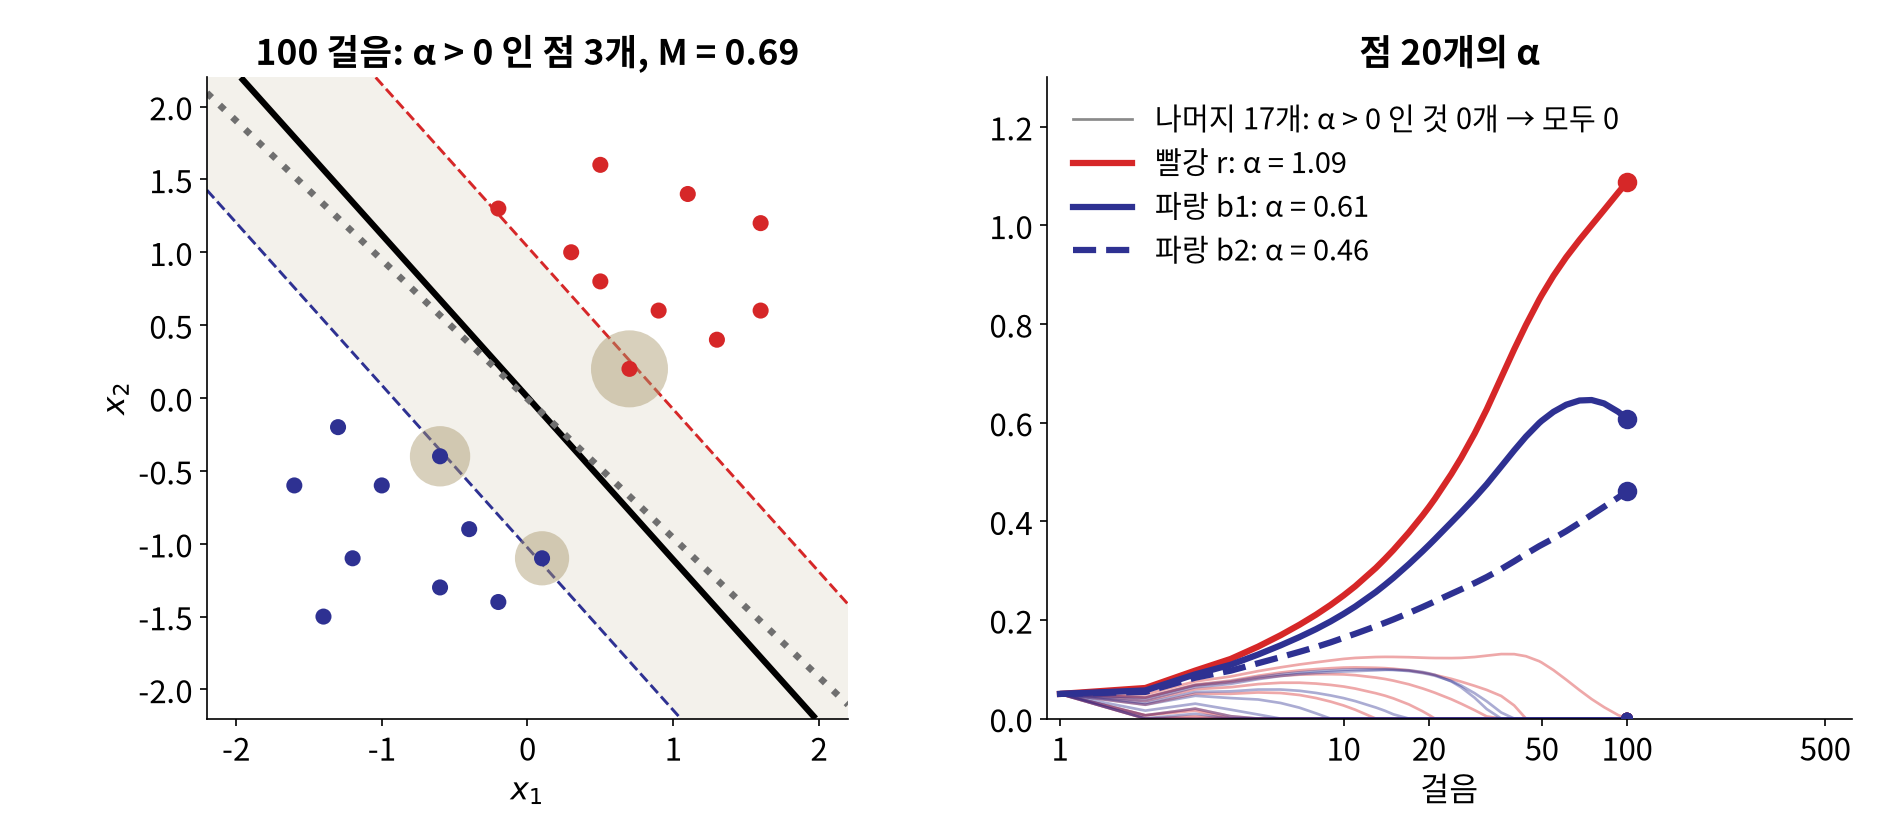
\includegraphics[width=0.88\linewidth]{kn_learn5.png}}%
\only<6>{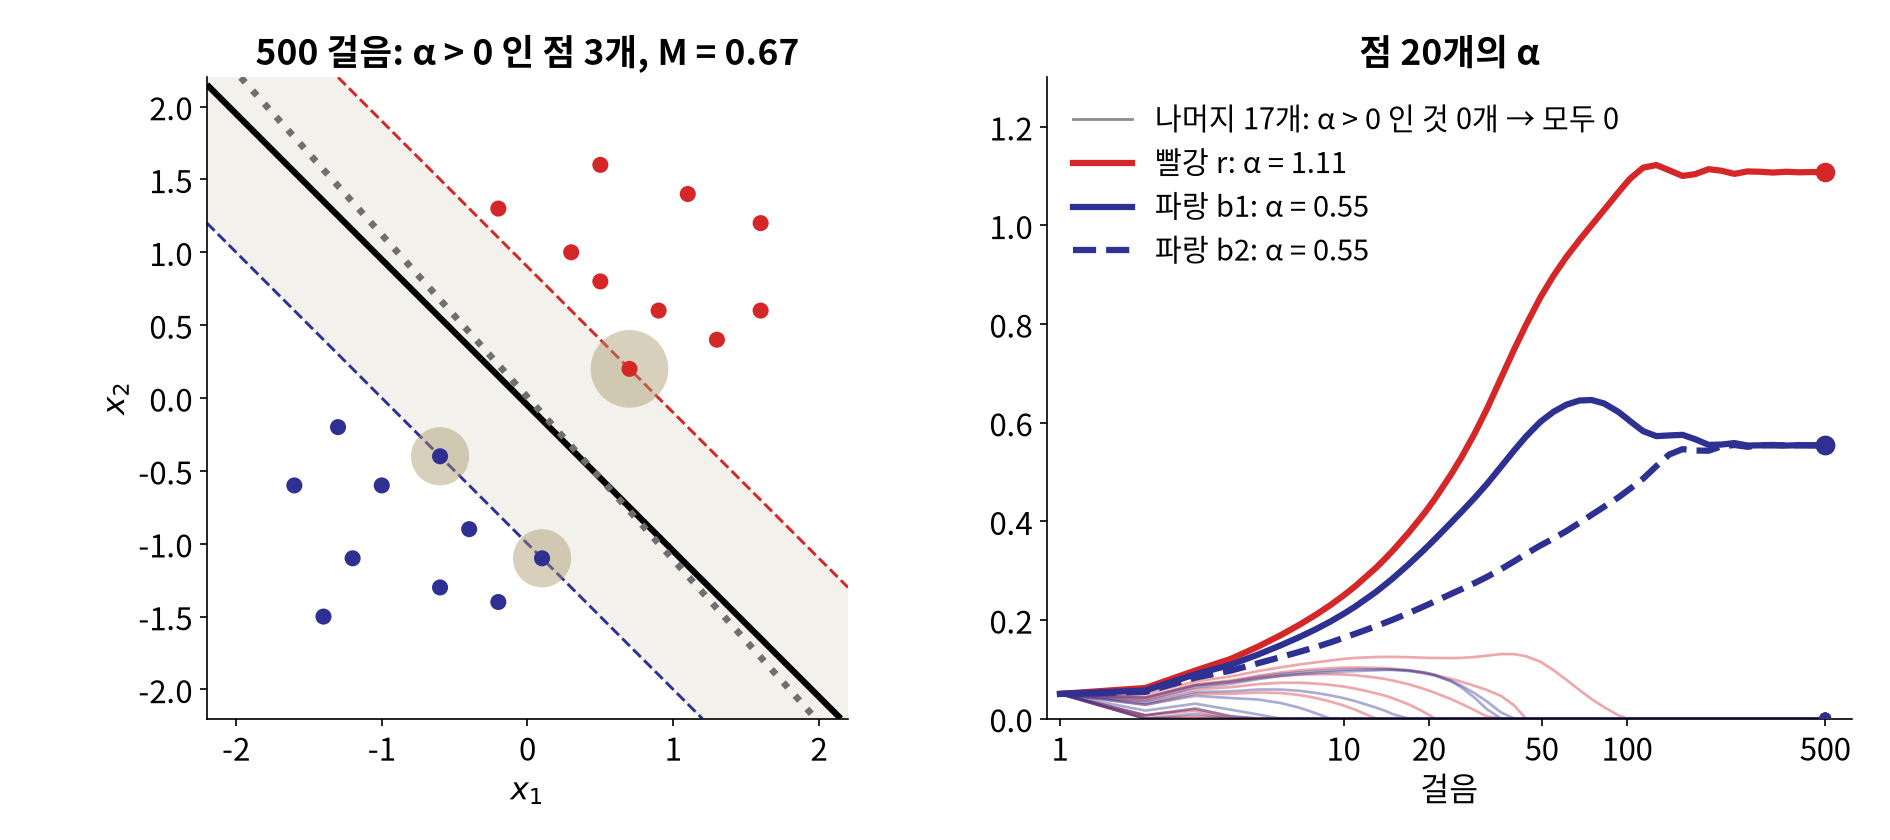
\includegraphics[width=0.88\linewidth]{kn_learn6.png}}%
\par\vskip0.4em
{\large \textcolor{ksagolddk}{\textbf{금색 원}} 크기 = $\alpha_k$ \qquad 점선 \textcolor{gray}{회색} = 앞 장면의 선}
\vfill
\note{알파를 학습하면서 선이 어떻게 자리를 잡는지 한 장면씩 넘겨 봅시다. 점 둘레의 금색 원이 클수록 그 점의 알파가 큽니다. 0걸음에는 20개가 모두 0.1이고, 선은 두 색의 평균을 가르는 선입니다. 한 걸음 뒤에는 길이 확 넓어지고 12개가 남습니다. 열 걸음에는 11개, 50걸음에는 4개입니다. 100걸음이면 서포트 벡터 3개만 남고, 이제는 세 점의 알파 사이의 균형만 맞춥니다. 500걸음에 알파가 1.11, 0.55, 0.55가 되고 선은 w 1.05, 1.05, b 0.05, 마진 0.67로 멈춥니다. 오른쪽 그래프의 가는 선은 나머지 17개 점의 알파입니다. 길 밖이 되면 하나씩 0으로 떨어집니다. 회색 점선은 바로 앞 장면의 선이라, 선이 얼마나 움직였는지 볼 수 있습니다.}
\end{frame}

% --- α 가 쌓이는 모습
\begin{frame}{$\alpha$ 가 자라는 모습: 서포트 벡터 3개만 남는다}
\vfill
\centering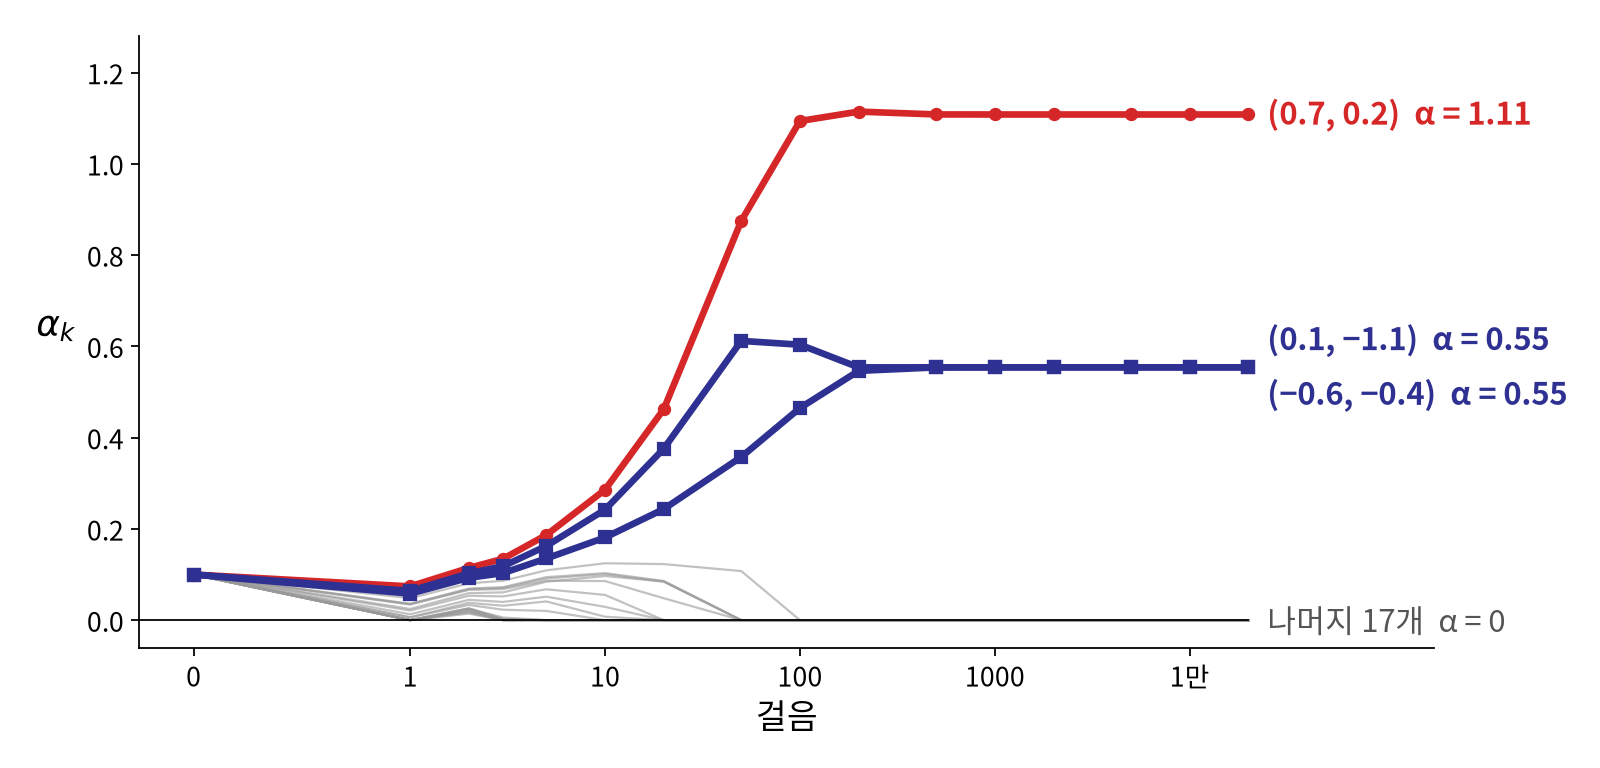
\includegraphics[width=0.78\linewidth]{kn_alpha.png}\par\vskip0.2em
{\large 서포트 벡터 3개: $\alpha = 1.11$ · $0.55$ · $0.55$ \;(= sklearn), 나머지 17개 \kb{0}}
\vfill
\note{같은 학습을 걸음마다 알파로 그렸습니다. 가로축은 걸음, 로그 눈금입니다. 0걸음에는 20개가 모두 0.1입니다. 첫 걸음에 다 같이 줄었다가, 그 뒤 빨간 서포트 벡터와 파란 서포트 벡터 둘의 알파는 계속 커지고, 회색 17개는 잠깐 커졌다가 값이 1을 넘으면서 줄어, 100걸음이면 모두 0이 됩니다. 알파는 0 아래로 못 가니 0에서 멈춥니다. 200걸음쯤이면 빨강 1.11, 파랑 0.55씩에서 평평해집니다. 빨강의 힘이 파랑 두 힘의 합과 같아지는 곳입니다. 그래서 w는 서포트 벡터 세 개에 알파를 곱해 더한 것이고, 나머지 17개 점은 w에 들어가지 않습니다.}
\end{frame}

% --- 닿은 점만 α > 0
\begin{frame}{정리하면: 가장자리에 닿은 점만 $\alpha_k > 0$}
\vfill
\centering
{\LARGE $\alpha_k\,\big(\,y_k D(\mathbf{x}_k) - 1\,\big) = 0, \qquad k = 1, \dots, p$}\\[1.1em]
\renewcommand{\arraystretch}{1.5}
{\large\begin{tabular}{c|c|c}
점 $\mathbf{x}_k$ & 여유 $y_k D(\mathbf{x}_k) - 1$ & 당기는 힘 $\alpha_k$\\ \hline
길 밖 (안 닿음) & $> 0$ & 반드시 \kb{0}\\
가장자리 (닿음) & $= 0$ & $> 0$ 일 수 있다 = \kq{서포트 벡터}
\end{tabular}}\\[1em]
{\large 곱이 0 이면 둘 중 하나는 0}\\[0.5em]
{\normalsize 이 데이터: 서포트 벡터 3개만 여유 $0$ $\to$ $\alpha = 1.1$ · $0.55$ · $0.55$, \;나머지 17개 $\alpha = 0$}
\vfill
\note{답에서는 원 논문 식 15가 성립합니다. 점마다 알파 k 곱하기 여유가 0입니다. 곱이 0이면 둘 중 하나는 0이어야 합니다. 길 밖에 있어서 여유가 0보다 큰 점은 알파가 반드시 0입니다. 알파가 0보다 클 수 있는 점은 여유가 0, 가장자리에 닿은 점뿐입니다. 그 점들이 서포트 벡터입니다. 역학 비유로 말하면 닿아 있을 때만 힘이 생깁니다. 이 데이터에서는 서포트 벡터 3개의 여유가 0이고 알파가 1.1, 0.55, 0.55입니다. 나머지 17개는 여유가 있어서 알파가 0입니다.}
\end{frame}

% --- 학습이 끝나면: w 와 분류기
\begin{frame}{학습이 끝나면: $\alpha^*$ 로 선 긋고, 새 점 분류하기}
\vfill
\centering
{\Large \textbf{선의 방향} \; $\displaystyle \mathbf{w}^* = \sum_{k=1}^{p} \alpha_k^* y_k \mathbf{x}_k$}\\[0.45em]
{\Large \textbf{분류기} \; $\displaystyle D(\mathbf{x}) = \mathbf{w}^* \cdot \mathbf{x} + b^* = \sum_{k=1}^{p} \alpha_k^* y_k\, (\mathbf{x}_k \cdot \mathbf{x}) + b^*$}\\[0.4em]
{\large $D(\mathbf{x}) > 0$ 이면 \kq{빨강}, $< 0$ 이면 \kb{파랑}}\\[0.4em]
\fcolorbox{fbeta}{fbeta!10}{\begin{minipage}{0.92\linewidth}\centering
{\large 학습이 끝난 분류기는 \textbf{길 가장자리에 걸친 점} (서포트 벡터) \textbf{만으로} 쓸 수 있다}\\[0.15em]
{\large $\to$ 그래서 처음부터 $\mathbf{w}$ 대신 \kq{$\alpha$ 로 학습}하는 방법도 가능하다}
\end{minipage}}\\[0.35em]
{\normalsize 이 데이터: $\mathbf{w}^* = (1.05,\ 1.05)$, \; $b^* = 0.05$ \;$\to$\; 새 점 $(0.5,\ -0.3)$: $D = 0.26$ \kq{빨강}}
\vfill
\note{학습이 끝나면 두 식만 있으면 됩니다. 첫째, 선의 방향 w 별은 알파 별 곱하기 y 곱하기 x를 모두 더한 것입니다. 앞에서 본 파랑 중심에서 빨강 중심으로 가는 화살표입니다. 둘째, 새 점 x를 분류할 때는 D x, w 별 점곱 x 더하기 b 별을 계산합니다. w 별 자리에 첫째 식을 넣으면 알파 별 곱하기 y 곱하기, 학습 점 x k와 새 점 x의 점곱을 더한 꼴이 됩니다. 0보다 크면 빨강, 작으면 파랑입니다. 알파가 0인 점은 합에서 사라집니다. 그래서 학습이 끝난 분류기는 길 가장자리에 걸친 점, 서포트 벡터만으로 쓸 수 있고, 나머지 점은 지워도 답이 같습니다. 거꾸로 생각하면, 어차피 점마다의 알파로 쓸 수 있으니 처음부터 w를 두지 않고 알파를 학습하는 방법도 가능합니다. 방금까지 J를 키운 것이 그 방법입니다. 이 데이터에서 w 별은 1.05, 1.05, b 별은 0.05이고, 새 점 0.5, 마이너스 0.3의 D는 0.26이라 빨강입니다. 원 논문의 식 16과 18입니다. 점이 점곱 안에만 있다는 것이 다음 시간 커널의 출발점입니다.}
\end{frame}

\section{소프트 마진}
% --- 최대 마진의 약점
\begin{frame}{최대 마진의 약점: 겹치면 불가능, 점 하나에 민감}
\vfill
\centering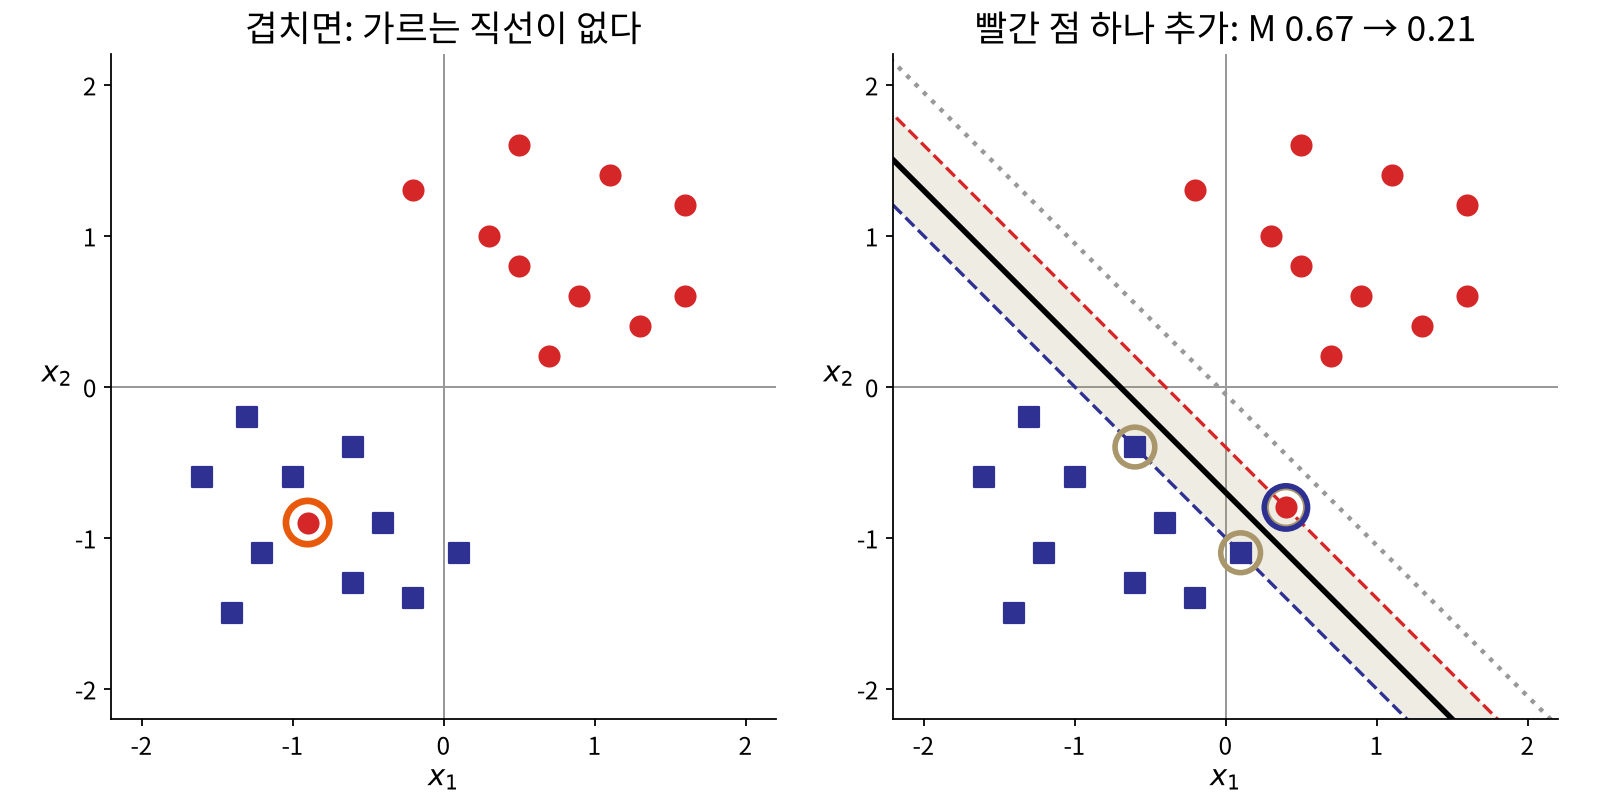
\includegraphics[width=0.66\linewidth]{sv_sensitive.png}\par\vskip0.2em
{\large 가를 수 \kq{없다} \quad 점 하나에 $M$ $0.67 \to 0.21$}
\vfill
\note{최대 마진 분류기에는 두 가지 약점이 있습니다. 첫째, 왼쪽처럼 빨간 점 하나가 파랑 무리 안에 들어오면 두 무리를 완벽히 가르는 직선이 아예 없습니다. 그러면 문제의 답이 없습니다. 둘째, 가를 수 있더라도 점 하나에 아주 민감합니다. 오른쪽은 빨간 점 하나를 0.4, 마이너스 0.8에 더한 것입니다. 마진이 0.67에서 0.21로 확 줄고, 경계도 점선이던 원래 경계에서 기울어집니다. 점 하나 때문에 경계가 크게 흔들리면 학습 데이터에 과대적합하기 쉽습니다.}
\end{frame}

% --- 서포트 벡터 분류기 식 (Cortes, Vapnik 1995)
\begin{frame}{서포트 벡터 분류기 (소프트 마진) 찾기}
\markpage{soft}
\vfill
\hspace*{0.3cm}\begin{minipage}{0.7\textwidth}
{\large\begin{align*}
\text{find} \quad & \mathbf{w},\ b,\ \xi_1, \dots, \xi_p\\ & \text{that minimize } \tikzmarknode{ob}{\tfrac{1}{2}\lVert\mathbf{w}\rVert^2 + C\sum_{k=1}^{p} \xi_k}\\[0.3em]
\text{subject to} \quad & y_k D(\mathbf{x}_k) \ge \tikzmarknode{me}{1 - \xi_k},\\[0.3em]
& \tikzmarknode{ep}{\xi_k \ge 0}
\end{align*}}
\end{minipage}
\begin{tikzpicture}[remember picture,overlay]
\node[bub,anchor=west] (s3) at ([xshift=0.5cm,yshift=0.4cm]ob.east) {넓은 길 \;$+$\; $C\,\times$ 넘어간 양};
\draw[bubarr] (s3.west) -- (ob.east);
\node[bub,anchor=west] (s1) at ([xshift=0.6cm,yshift=0.2cm]me.east) {값 1 이상이거나,\\ 아니면 모자란 값 $\xi_k$};
\draw[bubarr] (s1.west) -- (me.east);
\node[bub,anchor=north] (s2) at ([yshift=-0.5cm]ep.south) {\textbf{슬랙 변수} $\xi_k$: 점마다 하나};
\draw[bubarr] (s2.north) -- (ep.south);
\end{tikzpicture}
\vskip2.2em

\vfill
\note{깔끔하게 나뉘지 않을 때 쓰는 서포트 벡터 분류기, 소프트 마진의 식입니다. 1995년 Cortes와 Vapnik의 논문, Support-vector networks의 식을 그대로 씁니다. SVM이라는 이름도 이 논문에서 나왔습니다. 앞에서 본, 길 가장자리의 값을 1로 두는 식과 거의 같은데 두 군데가 다릅니다. 첫째, 조건의 오른쪽이 1이 아니라 1 빼기 크사이 k입니다. 점마다 값이 1 이상인 게 원칙인데, 못 지키면 모자란 만큼 크사이를 씁니다. 이 크사이를 슬랙 변수라고 하고 점마다 하나씩 있습니다. 둘째, 줄이는 것이 2분의 1 w 길이 제곱 하나가 아니라 C 곱하기 크사이의 합을 더한 것입니다. w가 작을수록 길이 넓으니 앞의 항은 넓은 길을 원하고, 뒤의 항은 점이 길 안으로 들어오거나 넘어간 양만큼 벌점을 줍니다. C는 그 벌점에 거는 무게입니다. C가 크면 한 점도 안 넘기려 해서 하드 마진에 가까운 좁은 길, C가 작으면 몇 점 넘어가더라도 넓은 길을 택합니다. sklearn의 C가 바로 이 C입니다.}
\end{frame}

% --- 슬랙 읽기
\begin{frame}{슬랙 $\xi_k$ 읽기: 넘어가도 되지만 손해}
\vfill
\begin{columns}[c]
\begin{column}{0.40\textwidth}\centering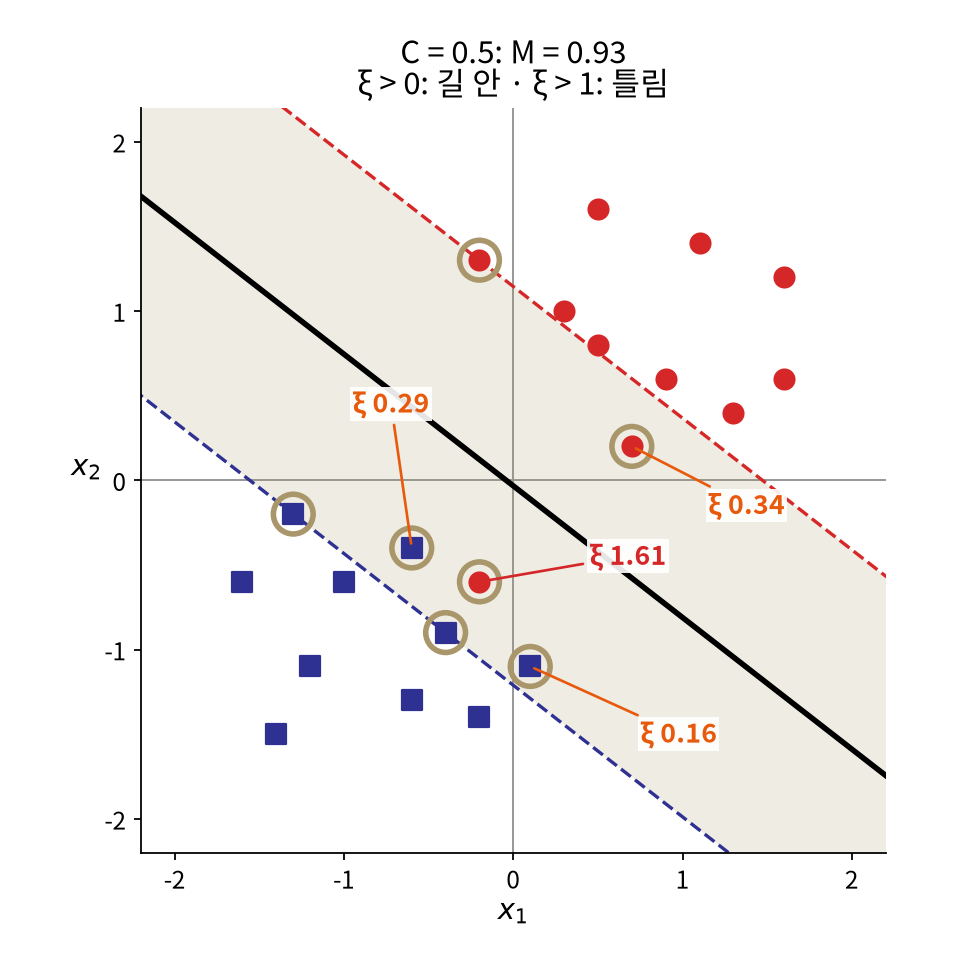
\includegraphics[width=0.95\linewidth]{sv_slack.png}\end{column}
\begin{column}{0.58\textwidth}
\renewcommand{\arraystretch}{1.3}
{\large\begin{tabular}{l|l}
$\xi_k = 0$ & 가장자리 바깥, 제자리\\
$0 < \xi_k \le 1$ & 가장자리를 넘어 길 안\\
$\xi_k > 1$ & 경계도 넘음 = \kq{틀림}\\
$C$ & 넘어간 양에 거는 \kb{벌점}
\end{tabular}}
\end{column}
\end{columns}
\vfill
\note{그림으로 크사이를 읽어 봅시다. 크사이는 값이 1에서 모자란 양입니다. 가장자리의 값이 1, 경계의 값이 0이니, 크사이가 0이면 원래대로 가장자리 바깥, 0보다 크고 1 이하면 가장자리를 넘어 길 안, 1보다 크면 경계까지 넘어 틀리게 분류된 것입니다. 그림은 C가 0.5일 때로, M이 0.93입니다. 파랑 무리 안의 빨간 점은 크사이 1.61로 1보다 커서 틀렸고, 나머지 세 점은 0.16에서 0.34만큼 길 안에 들어와 있습니다. 서포트 벡터는 가장자리 위의 점과 가장자리를 넘은 점 모두입니다.}
\end{frame}

% --- 벌점 C
\begin{frame}{$C$: 크면 좁은 길, 작으면 넓은 길}
\vfill
\centering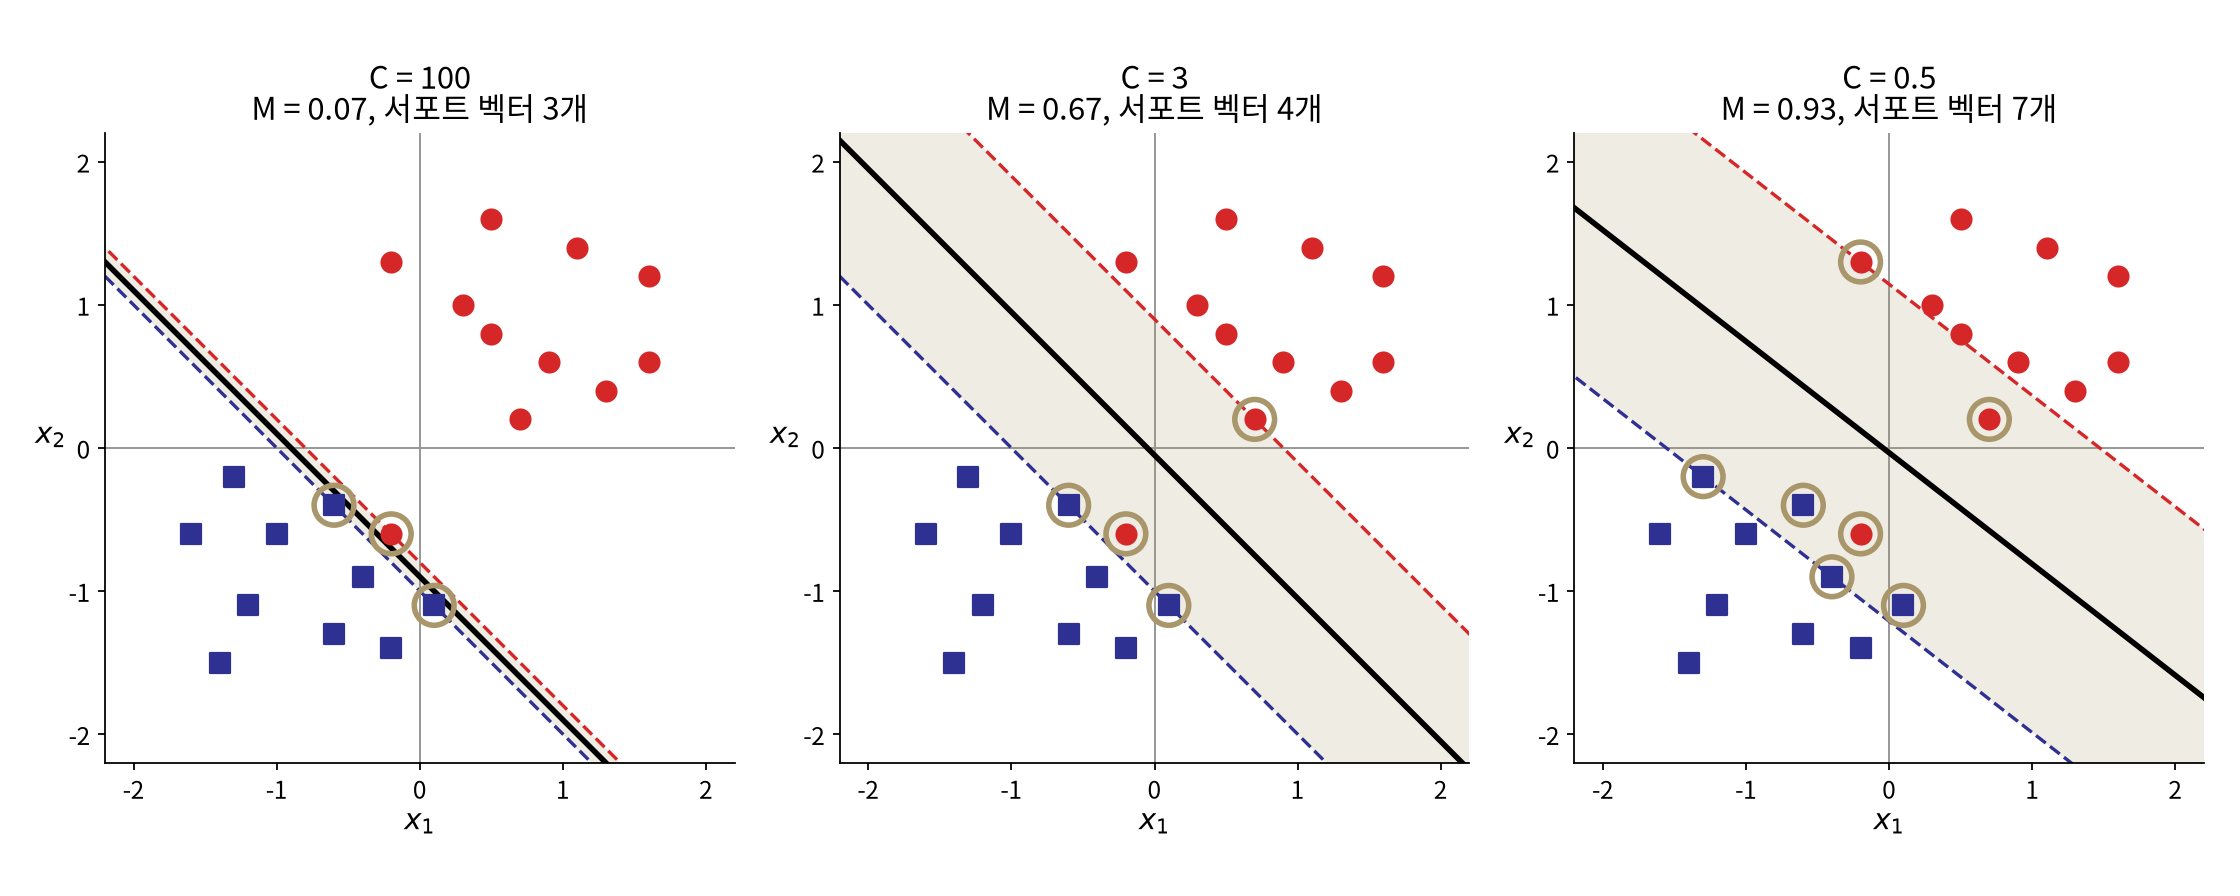
\includegraphics[width=0.8\linewidth]{sv_soft.png}\par\vskip0.1em
{\large $C$ = 넘어간 양의 벌점 \quad 크면 하드 마진에 가까운 \kq{좁은 길}, 작으면 \kb{넓은 길}}
\vfill
\note{C를 바꿔 봅시다. C가 100이면 넘어가는 벌점이 아주 커서, 이상치 하나까지 길 바깥에 두려고 길을 아주 좁힙니다. 마진이 0.07이고 서포트 벡터는 3개입니다. C가 3이면 이상치 하나를 틀리게 두고 원래 데이터와 같은 마진 0.67, 서포트 벡터 4개입니다. C가 0.5면 여러 점이 길 안에 들어오는 대신 마진이 0.93으로 넓어지고 서포트 벡터가 7개로 늘어납니다. C가 작으면 경계가 여러 점의 영향을 고루 받아 덜 흔들리니 분산은 작고 편향은 큽니다. C가 크면 반대입니다. C는 교차 검증으로 고릅니다. 세 그림 모두 덱 맨 뒤 다음 쪽의 학습으로 직접 구한 것이고, sklearn 결과와 같은 선입니다.}
\end{frame}

% --- 소프트 마진 학습 = α ≤ C
\begin{frame}{소프트 마진의 학습: $\alpha$ 가 $C$ 를 넘지 않게 자르기만}
\vfill
\centering
\renewcommand{\arraystretch}{1.55}
{\large\begin{tabular}{rl}
\textbf{1.} 힘 & $\alpha_k \leftarrow \textcolor{ksared}{\boldsymbol{\min\big(C,}}\ \max\big(0,\ \alpha_k + \eta\,(1 - y_k D(\mathbf{x}_k))\big)\textcolor{ksared}{\boldsymbol{\big)}}$\\
\textbf{2.} $b$ & $b \leftarrow b + \eta \sum_{k} \alpha_k y_k$ \quad (같다)
\end{tabular}}\\[0.9em]
{\large 푸는 $J$ 도 같다, 조건만 \;$\alpha_k \ge 0$ \;$\to$\; \kb{$0 \le \alpha_k \le C$}}\\[0.5em]
{\large 점이 미는 힘 $\alpha_k$ 에 한계 $C$: 더 세게 밀어야 하는 점은 \kq{$\alpha_k = C$} 로 길 안에 들어온다}\\[0.8em]
{\normalsize 이상치 포함 21개: $C = 100$ · $3$ · $0.5$ $\to$ $M = 0.07$ · $0.67$ · $0.93$ \;= sklearn 과 같은 선}
\vfill
\note{그러면 소프트 마진은 어떻게 학습할까요. 놀랍게도 하드 마진 학습에서 한 곳만 바꾸면 됩니다. 알파를 고칠 때 0 아래로 못 가게 막은 것처럼, 위로는 C를 넘지 못하게 자릅니다. b를 고치는 줄은 그대로입니다. 1995년 Cortes와 Vapnik의 논문에서 슬랙을 넣고 라그랑주를 다시 하면, 최대로 만드는 J는 똑같고 알파의 조건만 0 이상에서 0 이상 C 이하로 바뀝니다. 점이 경계를 미는 힘 알파에 한계 C가 있는 것입니다. 그보다 세게 밀려야 하는 점은 힘이 C에 딱 붙은 채로 길 안에 들어옵니다. 이상치가 있는 21개 점으로 이 두 줄을 돌리면 C가 100, 3, 0.5일 때 마진이 0.07, 0.67, 0.93으로, sklearn의 SVC와 같은 선이 나옵니다. C가 크면 한계가 높아서 한 점도 안 넘기려 하고, 작으면 일찍 포기하고 넓은 길을 택합니다. sklearn의 SVC가 푸는 조건이 바로 0 이상 C 이하입니다. w로 직접 학습하는 다른 방법은 덱 맨 뒤 Appendix에 있습니다. 못 비유로 말하면 못이 말랑해서 버틸 수 있는 힘에 한계 C가 있고, 그보다 세게 밀리면 못이 휘어 길 안으로 들어옵니다.}
\end{frame}

\section{$\alpha$ 의 뜻}
% --- 역학 비유
\begin{frame}{역학으로 보면: $\alpha$ = 서포트 벡터가 경계를 미는 힘}
\vfill
\centering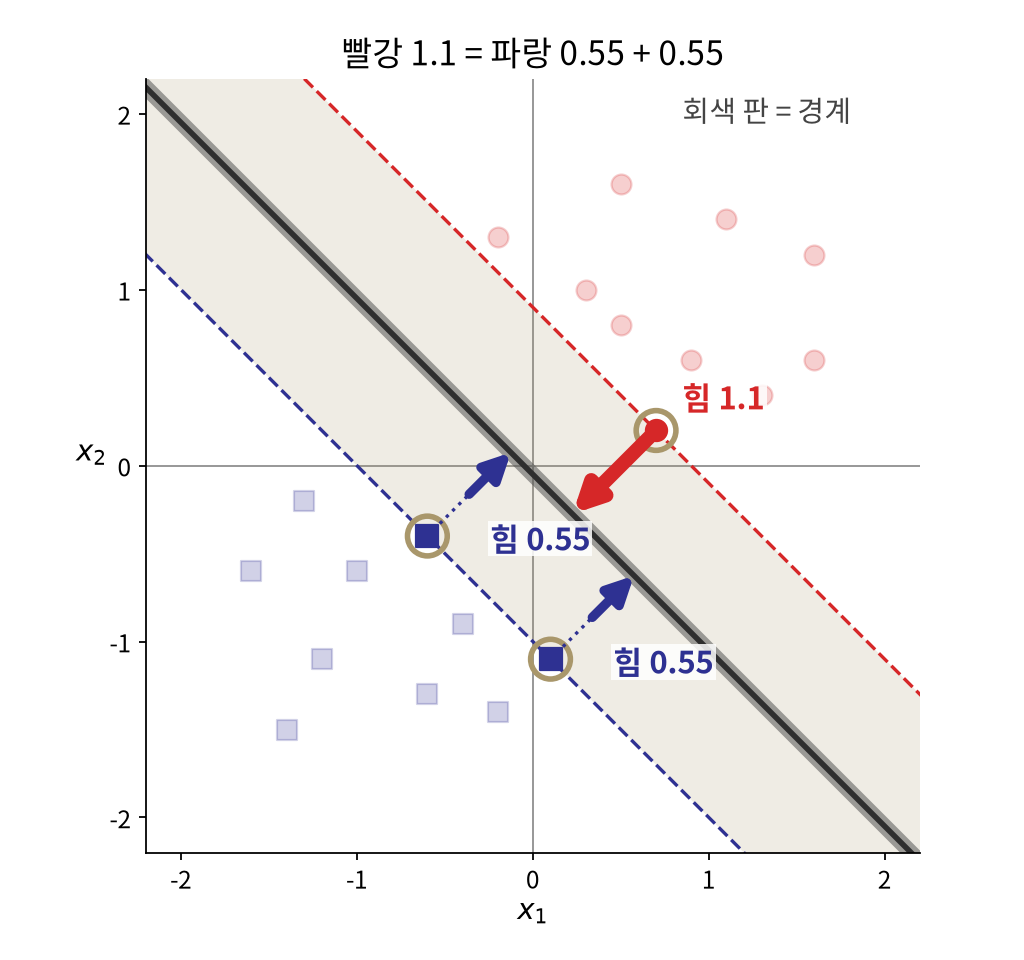
\includegraphics[height=0.62\textheight]{kn_force.png}\par\vskip0.2em
{\large 양쪽 힘이 같다 \ $1.1 = 0.55 + 0.55$, \;$\sum_k \alpha_k y_k = 0$ \;$\to$\; 경계가 \kb{멈춘다}}\\[0.2em]
{\normalsize 서포트 벡터 = 길을 \kq{받치는} 점 (support), \ 나머지 17개는 힘 0}
\vfill
\note{알파를 힘으로 보는 역학 비유가 있습니다. 경계를 딱딱한 판이라고 생각합시다. 서포트 벡터가 이 판을 밉니다. 빨간 서포트 벡터는 파랑 쪽으로, 파란 서포트 벡터 둘은 빨강 쪽으로 밉니다. 미는 힘의 크기가 알파이고, 미는 방향이 라벨 y입니다. 빨강은 1.1, 파랑은 각각 0.55입니다. 판이 어느 쪽으로도 밀려 가지 않으려면 양쪽 힘이 같아야 합니다. 1.1은 0.55 더하기 0.55와 같고, 알파 k 곱하기 y k를 다 더하면 0입니다. 원 논문에서는 b까지 최적으로 고르면 이 합이 0이 된다는 식으로 나옵니다. 판이 돌지도 않습니다. 경계를 따라 잰 위치에 힘을 곱한 돌림힘을 더해 보면, 빨강은 위치 마이너스 0.35에 힘 1.1, 파랑은 위치 0.14와 마이너스 0.85에 힘 0.55씩이라, 0.39 더하기 0.08 빼기 0.47로 0입니다. 그래서 이 자리에서 판이 멈춥니다. 서포트 벡터라는 이름도 여기서 옵니다. 길의 가장자리를 받쳐서, support해서, 길이 더 넓어지지 못하게 막는 점들입니다. 나머지 17개 점은 판을 밀지 않습니다. 힘이 0, 알파가 0입니다. 원 논문 식 15가 이것입니다. 가장자리에 닿지 않은 점은 알파가 0입니다. 지워도 판이 그대로입니다. 이 비유는 Burges가 1998년에 쓴 SVM 튜토리얼에 나옵니다. 앞에서 본 J 학습에서 값이 1보다 모자란 점의 알파가 커지고, 합이 안 맞으면 b가 움직이던 것이 바로 이 힘을 맞춰 가는 과정입니다.}
\end{frame}

% --- 선형 SVM 을 점곱으로
\begin{frame}{$\mathbf{w} = \sum_k \alpha_k y_k \mathbf{x}_k$ 를 분류기에 넣으면: 새 점과 서포트 벡터의 점곱}
\vfill
\centering
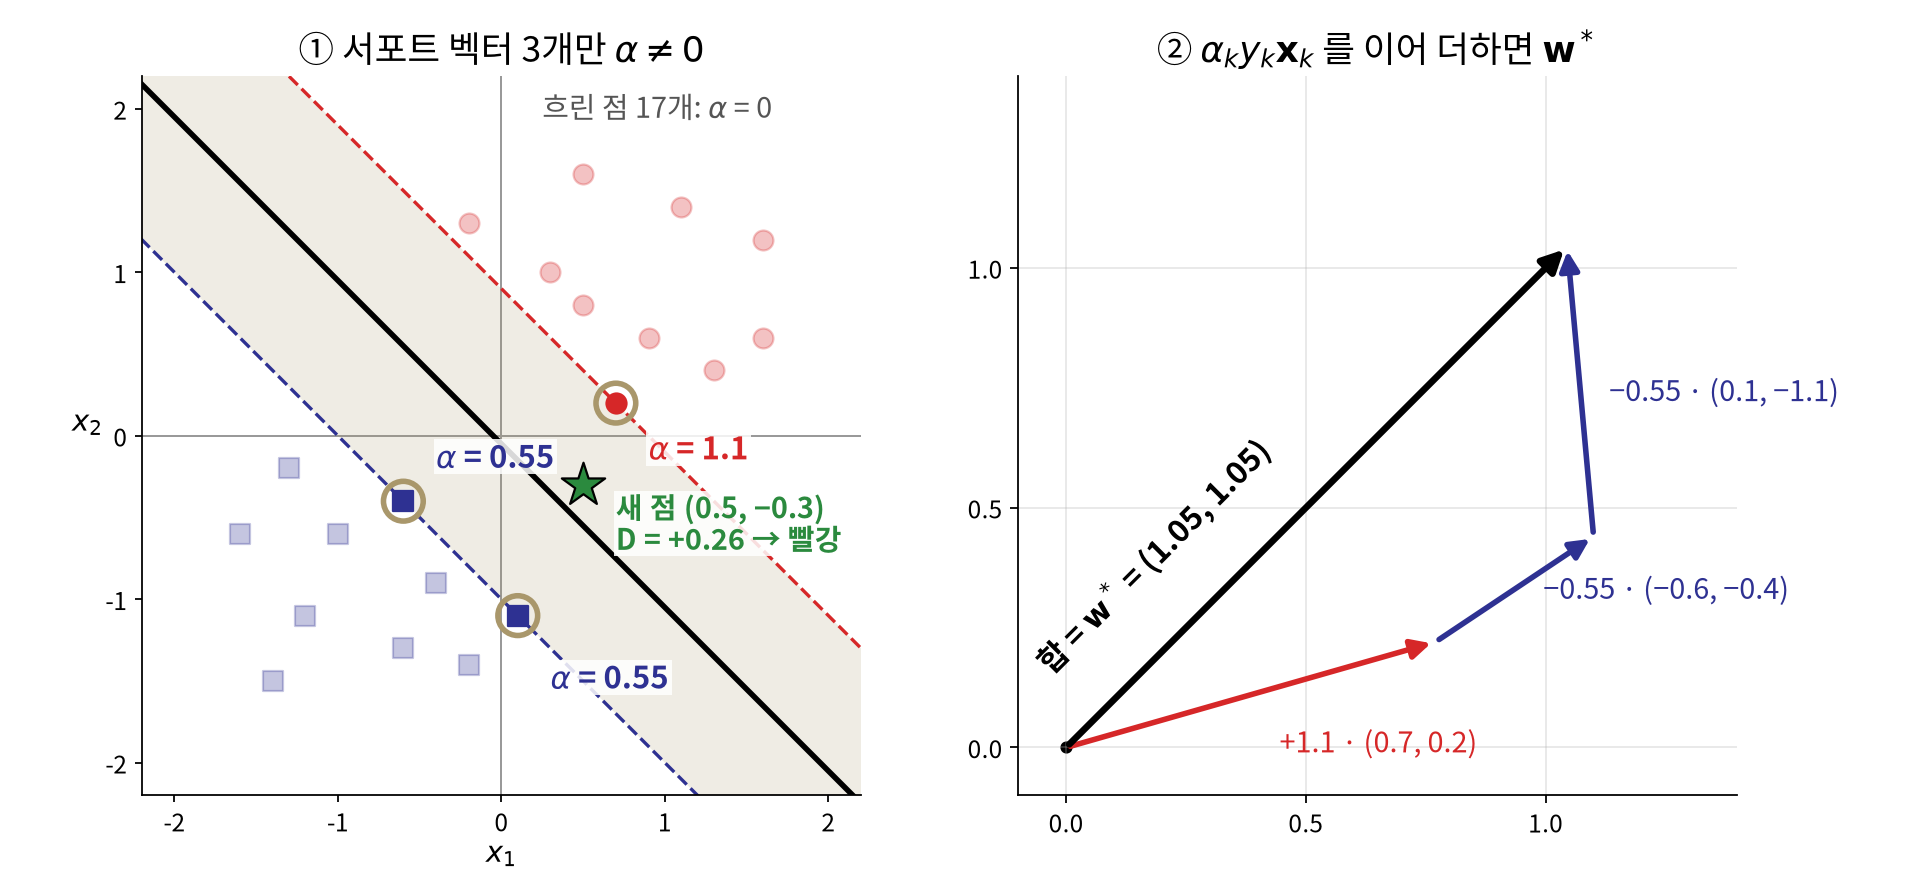
\includegraphics[width=0.62\linewidth]{kn_dual.png}\par\vskip0.1em
{\large $D(\mathbf{x}) = \mathbf{w}\cdot\mathbf{x} + b = \big(\sum_{k} \alpha_k y_k \mathbf{x}_k\big)\cdot\mathbf{x} + b = b + \sum_{k} \alpha_k y_k\, \mathbf{x}\cdot\mathbf{x}_k$}\\[0.1em]
{\normalsize 예 $\star$: \; $\mathbf{w}^*\cdot\mathbf{x} = 0.21$ (한 번에) $= 0.32 + 0.10 - 0.21$ (나눠서) $\to$ $D(\mathbf{x}) = +0.26$ \kq{빨강}}\\[0.1em]
{\small $\mathbf{x}$ = 분류할 새 점, \; $\mathbf{x}_k$ = 서포트 벡터 ($\alpha_k \neq 0$ 인 점만 남는다)}
\vfill
\note{방금 본 대로 w는 서포트 벡터에 알파와 y를 곱해 더한 것입니다. 이것을 분류기 D x, w 점곱 x 더하기 b에 넣어 봅시다. 왼쪽 그림에서 진한 점 3개가 서포트 벡터이고, 옆의 숫자가 그 점의 알파입니다. 빨간 서포트 벡터 0.7, 0.2는 알파가 1.1, 파란 둘은 0.55입니다. 흐리게 그린 나머지 17개는 알파가 0입니다. 경계를 정하는 데 쓰이지 않는 점들입니다. 오른쪽 그림은 알파 곱하기 y 곱하기 점을 화살표로 이어 붙인 것입니다. 빨강은 y가 플러스 1이라 그대로, 파랑은 마이너스 1이라 반대 방향입니다. 1.1 곱하기 0.7, 0.2에서 시작해 마이너스 0.55 곱하기 마이너스 0.6, 마이너스 0.4를 잇고, 마이너스 0.55 곱하기 0.1, 마이너스 1.1을 이으면, 끝점이 1.05, 1.05, 바로 w 별입니다. 그래서 w 점곱 x 더하기 b는 b 더하기 알파 k 곱하기 y k 곱하기 x 점곱 x k의 합으로 쓸 수 있습니다. 여기서 x는 분류하려는 새 점 하나, x k는 서포트 벡터 하나이고, 점곱은 숫자 하나입니다. 원 논문 식 18이 이 꼴입니다. 초록 별, 0.5, 마이너스 0.3을 분류해 봅시다. 빨간 서포트 벡터 0.7, 0.2와의 점곱은 0.35 빼기 0.06, 0.29이고 알파 1.1을 곱하면 0.32입니다. 파란 마이너스 0.6, 마이너스 0.4와의 점곱은 마이너스 0.18, 알파 0.55와 y 마이너스 1을 곱하면 0.10입니다. 파란 0.1, 마이너스 1.1과의 점곱은 0.38, 알파와 y를 곱하면 마이너스 0.21입니다. 더하면 0.21이고 b 별 0.05를 더하면 D는 0.26, 0보다 크니 빨강입니다. w 별 1.05, 1.05로 한 번에 계산해도 1.05 곱하기 0.5 더하기 1.05 곱하기 마이너스 0.3, 0.21로 같습니다. 이 기준에서 값은 거리가 아니라 가장 가까운 점을 1로 둔 눈금이라, 거리는 0.26 곱하기 마진 0.67, 0.18입니다. 왜 w 점곱 x가 이렇게 나뉠까요? 점곱은 더하기를 나눠서 할 수 있으니, 합 전체와 x의 점곱은 서포트 벡터마다 따로 계산해서 더한 것과 같습니다. 같은 값을 w로 한 번에 계산하느냐, 서포트 벡터마다 나눠 계산하느냐의 차이일 뿐입니다. 나눠 쓴 꼴에는 w가 없고 새 점과 서포트 벡터의 점곱만 남습니다. 이 점곱 자리를 바꾸는 것이 다음 시간에 볼 커널입니다.}
\end{frame}

\section{정리}
% --- 정리
\begin{frame}{정리}
\vfill
\centering\normalsize\begin{tabular}{l}
\textbf{크기 약속}: $M\lVert\mathbf{w}\rVert = 1$ $\to$ $\min \tfrac12\lVert\mathbf{w}\rVert^2$, 조건 $y_k D(\mathbf{x}_k) \ge 1$\\[0.6em]
\textbf{당기는 힘}: 점마다 $\alpha_k \ge 0$, \;$\mathbf{w} = \sum_k \alpha_k y_k \mathbf{x}_k$, \;닿은 점만 $\alpha_k > 0$\\[0.6em]
\textbf{학습}: 점수 $J$ 를 키운다 \;(길 안이면 $\alpha \uparrow$, 밖이면 $\alpha \downarrow$)\\[0.6em]
\textbf{소프트 마진}: $\min \tfrac12\lVert\mathbf{w}\rVert^2 + C\sum\xi_k$, $C$ 크면 좁은 길, 학습은 $\alpha_k \le C$\\[0.6em]
\textbf{분류}: $D(\mathbf{x}) = \sum_k \alpha_k y_k (\mathbf{x}_k\cdot\mathbf{x}) + b$, 서포트 벡터와의 \kb{점곱}만
\end{tabular}\par\vskip1em
{\large \kq{다음 시간}: 직선으로 못 가르면? $\to$ 커널}
\vfill
\note{정리합니다. 길 가장자리의 값을 1로 두는 약속을 하면 마진 최대는 2분의 1 w 길이 제곱 최소가 됩니다. 점마다 당기는 힘 알파가 있고, w는 그 힘의 합입니다. 점수 J를 키우는 것이 학습이고, 끝나면 가장자리에 닿은 점만 알파가 0보다 큽니다. 점이 겹치면 몇 점은 넘어가도 되게 하고 넘어간 양에 C만큼 벌을 주는 소프트 마진을 쓰고, 학습에서는 알파를 C에서 자르면 됩니다. 마지막으로 분류기에는 서포트 벡터와의 점곱만 남습니다. 다음 시간에는 이 점곱 자리를 바꿔서, 직선으로 못 가르는 데이터를 다루는 커널을 배웁니다.}
\end{frame}

\section{연습}
% --- 실습
\begin{frame}{실습}
\vfill
\centering\begin{tabular}{rl}
\large 1 & $\alpha$ 를 $J$ 로 직접 학습: 서포트 벡터 3개와 $\mathbf{w}^* = (1.05,\ 1.05)$ 확인\\[0.8em]
\large 2 & 이상치 하나 넣고 소프트 마진: $C$ 에 따른 길 폭과 서포트 벡터 수
\end{tabular}\vskip1.4em
\href{https://colab.research.google.com/github/SuminHan/book-ml/blob/main/slides/ml1/week02/3_svm_soft/lab/svm_soft.ipynb}{\textcolor{ksagolddk}{▶ Colab에서 실습 노트북 열기}}
\vfill
\note{실습은 두 부분입니다. 첫째, 지난 시간의 점 20개에서 알파를 J를 키우는 두 줄로 직접 학습해서, 서포트 벡터 3개만 알파가 남고 w가 1.05, 1.05가 되는지 sklearn과 비교합니다. 둘째, 빨간 이상치 하나를 파란 쪽에 넣고, C를 바꾸면 길 폭과 서포트 벡터 수가 어떻게 달라지는지 봅니다.}
\end{frame}
\appendix
\section{Appendix}
% ===== J 는 어디서 왔나 =====
% --- 점마다 α 만큼 당긴다: 식 하나로
\begin{frame}{점마다 $\alpha_k$ 만큼 당긴다고 생각하고, 식을 다시 쓰면}
\vfill
\centering
\vspace*{1.0cm}
{\large $L(\mathbf{w}, b, \boldsymbol{\alpha}) = \tikzmarknode{hw}{\tfrac{1}{2}\lVert\mathbf{w}\rVert^2} - \sum_{k=1}^{p} \tikzmarknode{al}{\alpha_k}\,\tikzmarknode{br}{\big[\,y_k D(\mathbf{x}_k) - 1\,\big]}$}\\[0.2em]
\begin{tikzpicture}[remember picture,overlay]
\node[bub,anchor=south east,font=\small] (c1) at ([xshift=0.15cm,yshift=0.45cm]hw.north) {\textbf{스프링}: $\lVert\mathbf{w}\rVert$ 작게 = 길 넓히기};
\draw[bubarr] (c1.south east) -- (hw.north);
\node[bub,anchor=south west,font=\small] (c3) at ([xshift=-1.0cm,yshift=0.45cm]br.north) {못의 \textbf{여유}: $0$ 닿음, $+$ 길 밖, $-$ 길 안};
\draw[bubarr] ([xshift=1.0cm]c3.south west) -- (br.north);
\node[bub,anchor=north,font=\small] (c2) at ([yshift=-0.45cm]al.south) {못 $\mathbf{x}_k$ 가 \textbf{당기는 힘} ($\alpha_k \ge 0$)};
\draw[bubarr] (c2.north) -- (al.south);
\end{tikzpicture}\par\vspace{1.35cm}
{\large $\displaystyle\min_{\mathbf{w},\,b}\ \max_{\boldsymbol{\alpha} \ge 0}\ L$ : \; $\mathbf{w}, b$ 는 $L$ 을 \kb{작게}, \; $\alpha_k$ 는 \kq{크게}}\\[0.5em]
{\large 길 안의 못 (여유 $-$): $\alpha_k$ 가 커진다 \quad 길 밖의 못 (여유 $+$): $\alpha_k$ 가 $0$ 으로}\\[0.8em]
{\small\color{gray} 참고: 이 $L$ = 라그랑주 함수 (Lagrangian), \; $\alpha_k$ = 라그랑주 승수}
\vfill
\note{못과 자 그림을 식으로 옮겨 봅시다. 모든 못이 자를 알파만큼 당긴다고 생각하면, 하고 싶은 일을 식 하나로 다시 쓸 수 있습니다. 첫 항 2분의 1 w 길이 제곱은 스프링입니다. w를 작게 할수록 길이 넓어집니다. 대괄호 안, y k D x k 빼기 1은 못 하나의 여유입니다. 0이면 자에 닿아 있고, 플러스면 길 밖에 여유가 있고, 마이너스면 길 안에 들어와 있습니다. 알파 k는 그 못이 당기는 힘이고, 0 이상입니다. 못은 자를 당기기만 하고 밀어내지는 않습니다. 이제 w와 b는 L을 작게, 알파는 크게 만듭니다. 왜 그런지 두 경우를 봅시다. 못이 길 안에 있으면 여유가 마이너스라서, 알파를 키울수록 L이 커집니다. 그래서 그 못은 점점 세게 당기고, 자는 그 못을 길 밖으로 내보내는 쪽으로 움직입니다. 못이 길 밖에 있으면 여유가 플러스라서, L을 크게 하려면 알파를 줄여야 하고, 0이 되면 더는 당기지 않습니다. 이렇게 조건마다 숫자를 붙여 식 하나로 만든 것을 수학에서는 라그랑주 함수, 알파를 라그랑주 승수라고 부릅니다. 일반적인 모양과 안장점 그림은 덱 맨 뒤 Appendix에 있습니다. 원 논문의 식 14입니다.}
\end{frame}

% --- J 는 L 에서 w 를 없앤 것
\begin{frame}{$J$ 는 $L$ 의 $\mathbf{w}$ 자리에 $\alpha$ 로 만든 $\mathbf{w}$ 를 넣은 것}
\vfill
\centering
{\Large $L(\mathbf{w}, b, \boldsymbol{\alpha})$ \quad $\xrightarrow{\ \ \mathbf{w} \,=\, \sum_k \alpha_k y_k \mathbf{x}_k\ \ }$ \quad \kq{$J(\boldsymbol{\alpha}, b)$}}\\[0.3em]
{\small $L$ 을 $\mathbf{w}$ 로 미분 $= 0$ 이면 $\mathbf{w} = \sum_k \alpha_k y_k \mathbf{x}_k$}\\[1.3em]
{\Large \kq{$J$} $=$ \textbf{$\alpha$ 를 모두 더한 값} $-$ $\tfrac12\lVert\mathbf{w}\rVert^2$}\\[0.2em]
{\small 양쪽 힘이 같을 때 ($\sum_k \alpha_k y_k = 0$)}\\[1.1em]
{\large 점 20개의 답: \; $(1.11 + 0.55 + 0.55) - 1.11 = 2.22 - 1.11 = \mathbf{1.11}$}\\[1em]
{\large $\alpha$ 를 키우면 \textbf{앞 항}이 오르고, 너무 키우면 \textbf{뒤 항}이 깎는다 \;$\to$\; \kb{꼭대기}}
\vfill
\note{J는 새로운 것이 아닙니다. L에는 손잡이가 w와 알파 두 개인데, w는 알파로 계산되니 그 자리에 넣으면 손잡이가 알파 쪽만 남습니다. 그것이 J입니다. w는 L을 w로 미분해 0으로 둔 값, 알파 y x의 합입니다. 양쪽 힘이 같을 때, 즉 알파 y의 합이 0일 때 J는 아주 간단합니다. 알파를 모두 더한 값에서 2분의 1 w 길이 제곱을 뺍니다. 점 20개의 답을 넣으면 알파의 합이 2.22, 뒤 항이 1.11이라 J는 1.11입니다. 앞 항은 알파를 키울수록 오릅니다. 하지만 알파를 키우면 w가 커져서 뒤 항이 더 크게 깎습니다. 그래서 어딘가에 꼭대기가 있고, 그 꼭대기의 알파가 답입니다. 컴퓨터는 알파만 만지면서 이 점수를 올립니다.}
\end{frame}

% --- 미분
\begin{frame}{미분하면 $\mathbf{w}$, $\mathbf{w}$ 를 지우면 $J$: 점은 점곱 안에만}
\vfill
\centering
{\large\begin{gather*}
\frac{\partial L}{\partial \mathbf{w}} = \mathbf{w} - \sum_{k} \alpha_k y_k \mathbf{x}_k = 0 \quad\to\quad \mathbf{w}^* = \sum_{k} \alpha_k y_k \mathbf{x}_k\\[0.3em]
J(\boldsymbol{\alpha}, b) = \sum_{k} \alpha_k\,(1 - b\,y_k) - \tfrac{1}{2}\,\boldsymbol{\alpha}\cdot\mathbf{H}\cdot\boldsymbol{\alpha}, \\[0.3em]
\mathbf{H} \in \mathbb{R}^{p \times p}, \qquad H_{kl} = y_k y_l\, \mathbf{x}_k\cdot\mathbf{x}_l
\end{gather*}}\\[0.3em]
{\large 할 일: $J$ 를 $\alpha_k \ge 0$ 에서 \kb{최대로} \quad 점은 \textbf{점곱} $\mathbf{x}_k\cdot\mathbf{x}_l$ 안에만}\\[0.35em]
{\normalsize 이 데이터: $\mathbf{w}^* = 1.1\,r - 0.55\,b_1 - 0.55\,b_2 = (1.05,\ 1.05)$}
\vfill
\note{방금 쓴 식 L을 w로 미분해서 0으로 두면, w 빼기 알파 k y k x k의 합이 0, 즉 w 별은 알파 k y k x k의 합입니다. 알파는 미는 힘이고 y는 미는 방향이니, w는 점들을 힘만큼 더한 것입니다. 이 w를 다시 L에 넣으면 w가 사라지고 알파와 b만 남는 J가 됩니다. 앞의 합은 알파 k 곱하기 1 빼기 b y k이고, 뒤는 알파 점 H 점 알파의 절반인데, H k l은 y k y l 곱하기 두 점의 점곱입니다. 이제 문제는 이 J를 알파가 0 이상인 범위에서 가장 크게 만드는 것입니다. 점이 들어가는 곳이 점곱 하나뿐이라는 것이 중요합니다.}
\end{frame}

% --- 점 두 개: 이차함수 꼭대기
\begin{frame}{점 두 개면: 이차함수의 꼭대기 찾기}
\vfill
\centering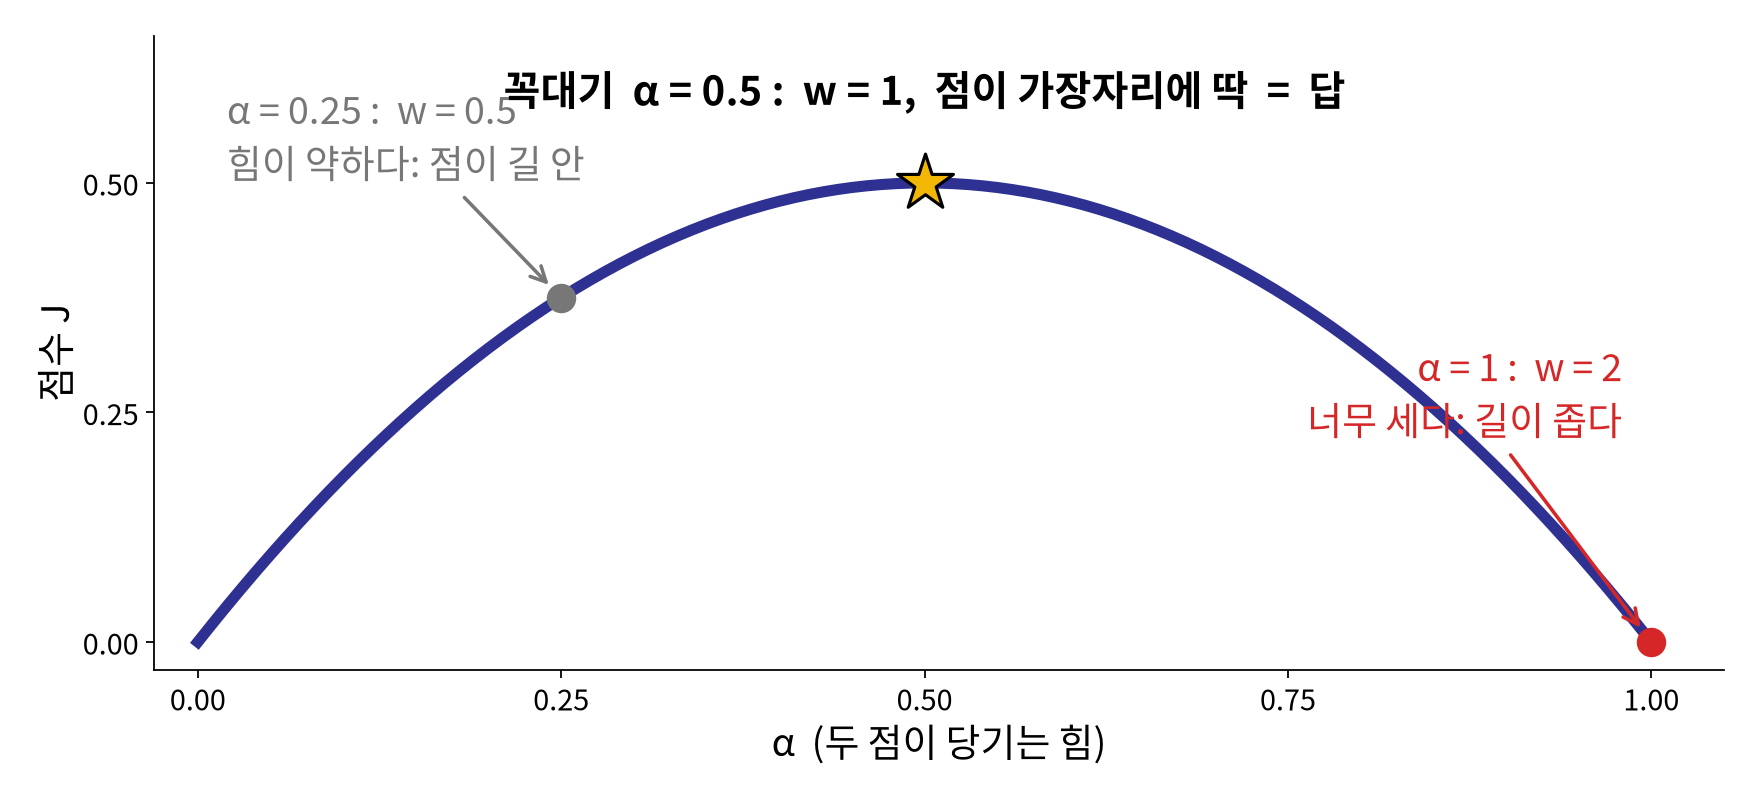
\includegraphics[width=0.60\linewidth]{kn_parab.png}\par\vskip0.3em
{\large 빨강 $x = +1$, 파랑 $x = -1$ (특징 1개), 두 힘은 같다}\\[0.25em]
{\large $\mathbf{w} = \alpha(+1)(+1) + \alpha(-1)(-1) = 2\alpha$ \qquad {\normalsize 숫자 하나}}\\[0.25em]
{\large $J = \underbrace{\alpha + \alpha}_{\text{힘의 합}} - \tfrac12 \lVert\mathbf{w}\rVert^2 = 2\alpha - \tfrac12 (2\alpha)^2 = \textcolor{ksared}{2\alpha - 2\alpha^2}$}
\vfill
\note{점이 두 개면 손으로 풀 수 있습니다. 빨간 점은 1, 파란 점은 마이너스 1에 있고, 규칙 때문에 두 힘은 같은 알파입니다. w는 알파 곱하기 1 곱하기 1 더하기 알파 곱하기 마이너스 1 곱하기 마이너스 1, 2 알파입니다. J는 힘의 합 2 알파에서 2분의 1 곱하기 2 알파의 제곱을 뺀 것, 2 알파 빼기 2 알파 제곱입니다. 중학교에서 배운 이차함수입니다. 그래프의 꼭대기는 알파가 0.5이고, 그때 w는 1, 길 반폭은 1 나누기 w라 1입니다. 두 점이 정확히 길 가장자리에 놓입니다. 알파가 0.25면 힘이 약해서 길이 넓고 점이 길 안에 있고, 1이면 너무 세게 당겨 길이 좁아집니다. 점이 20개면 손잡이가 20개라 그래프를 그릴 수 없어서, 컴퓨터가 조금씩 올라갑니다.}
\end{frame}

% --- J = α 의 성적표
\begin{frame}{$J(\alpha)$ 란: $\alpha$ 의 성적표}
\vfill
\centering
{\large 점 두 개 ($x = \pm 1$): \quad $L = \tfrac12 w^2 - 2\alpha\,(w - 1)$}\\[0.35em]
{\large $w - 2\alpha = 0$ \;$\to$\; $w = 2\alpha$ 를 넣으면 \quad \kq{$J(\alpha) = 2\alpha - 2\alpha^2$}}\\[0.7em]
\renewcommand{\arraystretch}{1.2}
{\large\begin{tabular}{c|c|c|l}
정한 $\alpha$ & $w$ 의 선택 ($= 2\alpha$) & \kq{$J(\alpha)$} & \\ \hline
$0$ & $0$ & $0$ & 벌이 없다: 규칙 무시\\
$0.25$ & $0.5$ & $0.375$ & 벌이 약하다\\
\textbf{0.5} & \textbf{1} & \textbf{0.5} & \textbf{최고점: 규칙을 딱 지킨다}\\
$1$ & $2$ & $0$ & 벌이 너무 세다
\end{tabular}}\\[0.9em]
{\large 학습 $=$ \kb{$J$ 가 가장 높은 $\alpha$ 찾기}}
\vfill
\note{방금 점 p개로 w를 지워 J를 만들었습니다. 점 두 개짜리 예로 같은 일을 해 봅니다. 빨간 점은 x가 플러스 1, 파란 점은 마이너스 1이고, b는 0, 두 점의 알파는 같습니다. L을 w로 미분해 0으로 두면 w 빼기 2 알파가 0, w는 2 알파이고, 이것을 L에 넣으면 J는 2 알파 빼기 2 알파 제곱입니다. J가 무엇인지 표로 정리합니다. J는 알파의 성적표, 숫자 하나입니다. 알파, 즉 벌의 세기를 하나 정하면, w는 L이 가장 낮아지는 값을 고릅니다. 이 예에서는 w가 2 알파입니다. 그때의 L 값이 J입니다. 알파가 0이면 벌이 없으니 w는 0을 골라 규칙을 무시하고, J는 0입니다. 0.25면 w가 0.5, 아직 규칙에 모자라고 J는 0.375입니다. 0.5면 w가 1로 규칙을 딱 지키고 J가 0.5로 가장 높습니다. 1이면 벌이 너무 세서 w가 2까지 가고 J는 다시 0입니다. 그래서 학습은 J가 가장 높은 알파를 찾는 것입니다. 딥러닝의 손실이 가중치가 얼마나 나쁜지를 숫자 하나로 말하듯, J는 알파가 얼마나 좋은지를 말합니다. 낮추는 대신 올립니다. J에는 w가 없습니다. w는 이미 가장 좋게 골라서 알파로 바꿔 썼기 때문입니다.}
\end{frame}

% --- 안장점 그림
\begin{frame}{안장점 (saddle point): 한 방향은 최소, 다른 방향은 최대}
\vfill
\centering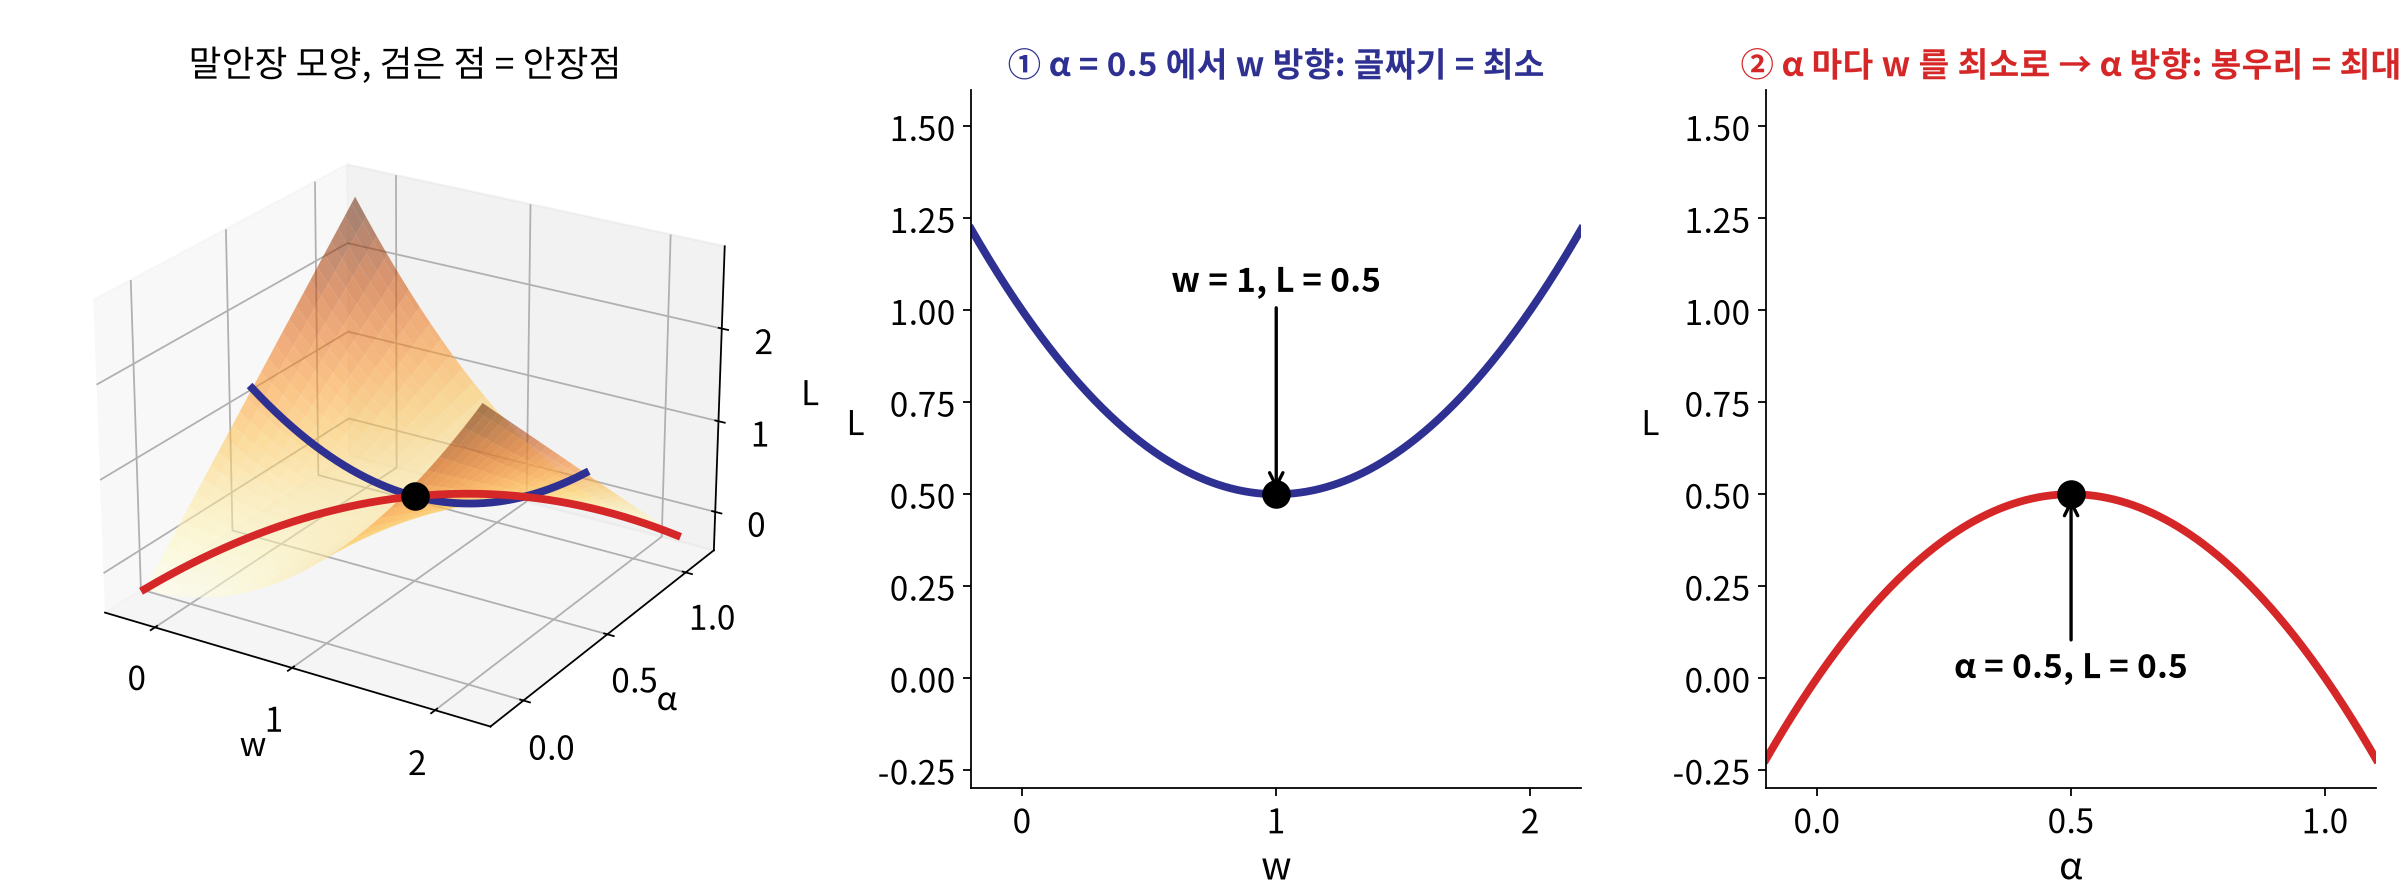
\includegraphics[width=0.80\linewidth]{kn_saddle.png}\par\vskip0.3em
{\large 점 두 개 ($x = \pm 1$): 조건 $w \ge 1$ \;$\to$\; $L(w, \alpha) = \tfrac12 w^2 - 2\alpha\,(w - 1)$}\\[0.3em]
{\large \textcolor{ksablue}{\textbf{$w$ 바닥}}: $w - 2\alpha = 0$ \;$\to$\; $L$ 에 $w = 2\alpha$ 를 넣으면 \textcolor{ksared}{$\mathbf{J(\alpha) = 2\alpha - 2\alpha^2}$}}\\[0.3em]
{\large 답 $w = 1$, $\alpha = 0.5$: \textcolor{ksablue}{\textbf{$w$ 방향 최소}}, \;\textcolor{ksared}{\textbf{$\alpha$ 방향 최대}}}
\vfill
\note{안장점을 그림으로 봅시다. 점 20개의 L은 숫자가 너무 많아 그릴 수 없으니, 점 두 개짜리 가장 작은 예를 씁니다. 빨간 점은 x가 플러스 1, 파란 점은 마이너스 1이고, b는 0입니다. 두 점 모두 y D가 w라서 조건은 w가 1 이상 하나이고, 2분의 1 w 제곱을 최소로 합니다. 두 점의 알파는 같습니다. 답은 눈으로도 w가 1입니다. 라그랑주 함수는 2분의 1 w 제곱 빼기 2 알파 곱하기 w 빼기 1입니다. 점이 둘이라 2가 붙습니다. 왼쪽 그림이 이 함수를 w와 알파에 대해 그린 곡면이고, 말안장처럼 한쪽으로는 휘어 올라가고 다른 쪽으로는 휘어 내려갑니다. 가운데 그림은 알파를 0.5로 두고 w를 움직인 것입니다. w가 1에서 가장 낮은 골짜기, 최소입니다. 오른쪽 그림은 알파를 하나 정할 때마다 w를 L이 가장 작게 되도록 고른 뒤, 그 값을 알파에 대해 그린 것입니다. w가 2 알파일 때 최소라서 2 알파 빼기 2 알파 제곱이 됩니다. 알파가 0.5에서 가장 높은 봉우리, 최대입니다. 그 값 0.5는 2분의 1 w 제곱, 즉 원래 문제의 답과 같습니다. 이렇게 w를 늘 바닥에 놓고 잰 L에 J라는 이름을 붙입니다. 식으로는 w로 미분한 w 빼기 2 알파가 0, 그래서 w는 2 알파이고, 이것을 L에 넣으면 2 알파 빼기 2 알파 제곱입니다. w를 먼저 없애고 알파만 남긴 함수를 최대로 만드는 것입니다.}
\end{frame}

% --- 안장 위의 점마다 상태
\begin{frame}{안장 위의 점 $(w, \alpha)$ 마다: 길은 어떤 모습일까}
\vfill
\centering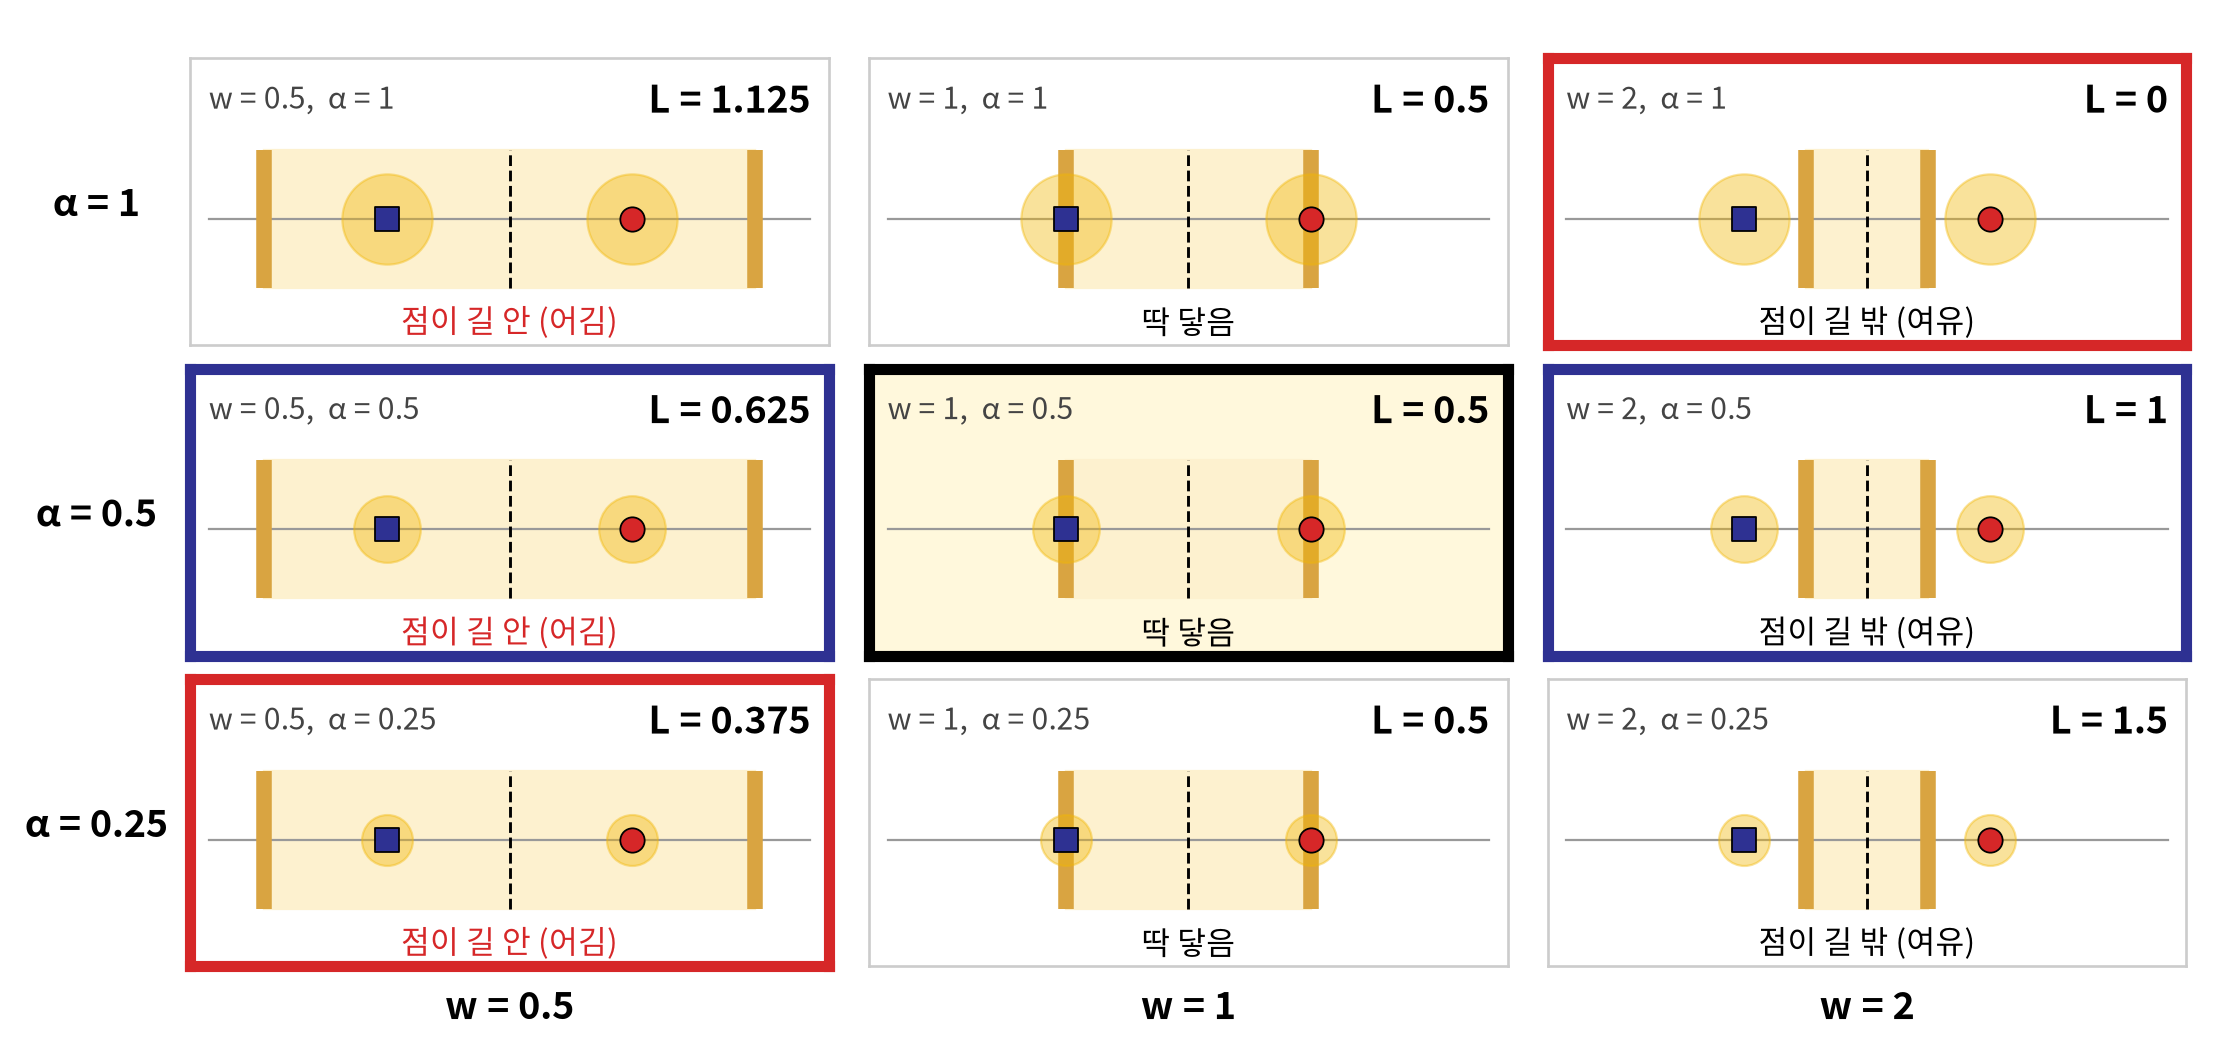
\includegraphics[width=0.78\linewidth]{kn_states.png}\par\vskip0.2em
{\normalsize \kb{파랑 줄}: $L$ 가운데가 최소 \quad \kq{빨강 대각선} ($J$): 가운데가 최대 \quad 겹친 칸 = \textbf{답}}
\vfill
\note{말안장 위의 점 하나는 w와 알파 한 쌍입니다. 점마다 길이 어떤 모습인지 아홉 칸으로 봅시다. 가로로 갈수록 w가 커져서 길이 좁아지고, 위로 갈수록 알파가 커져서 금색 원이 커집니다. 왼쪽 칸들은 길이 너무 넓어 점이 길 안에 들어와 있습니다. 규칙을 어긴 상태입니다. 가운데 칸들은 자가 점에 딱 닿아 있고, 오른쪽 칸들은 점이 길 밖에 있어 여유가 있습니다. 파란 테두리 줄은 알파를 0.5로 고정하고 w만 바꾼 것입니다. L이 0.625, 0.5, 1로, 가운데가 가장 낮습니다. 골짜기입니다. 빨간 테두리 대각선은 알파마다 w가 가장 낮게 고른 칸, w가 2 알파인 곳입니다. L이 0.375, 0.5, 0으로, 가운데가 가장 높습니다. 이것이 J이고 봉우리입니다. 두 테두리가 겹치는 가운데 칸, w가 1, 알파가 0.5가 안장점, 답입니다. 참고로 가운데 세로줄은 L이 모두 0.5입니다. 점이 딱 닿아 있으면 여유가 0이라 알파를 곱해도 아무것도 더해지지 않기 때문입니다.}
\end{frame}

% --- 위아래에서 만난다
\begin{frame}{업다운 게임처럼: 위와 아래에서 좁혀 가면 한 값}
\vfill
\centering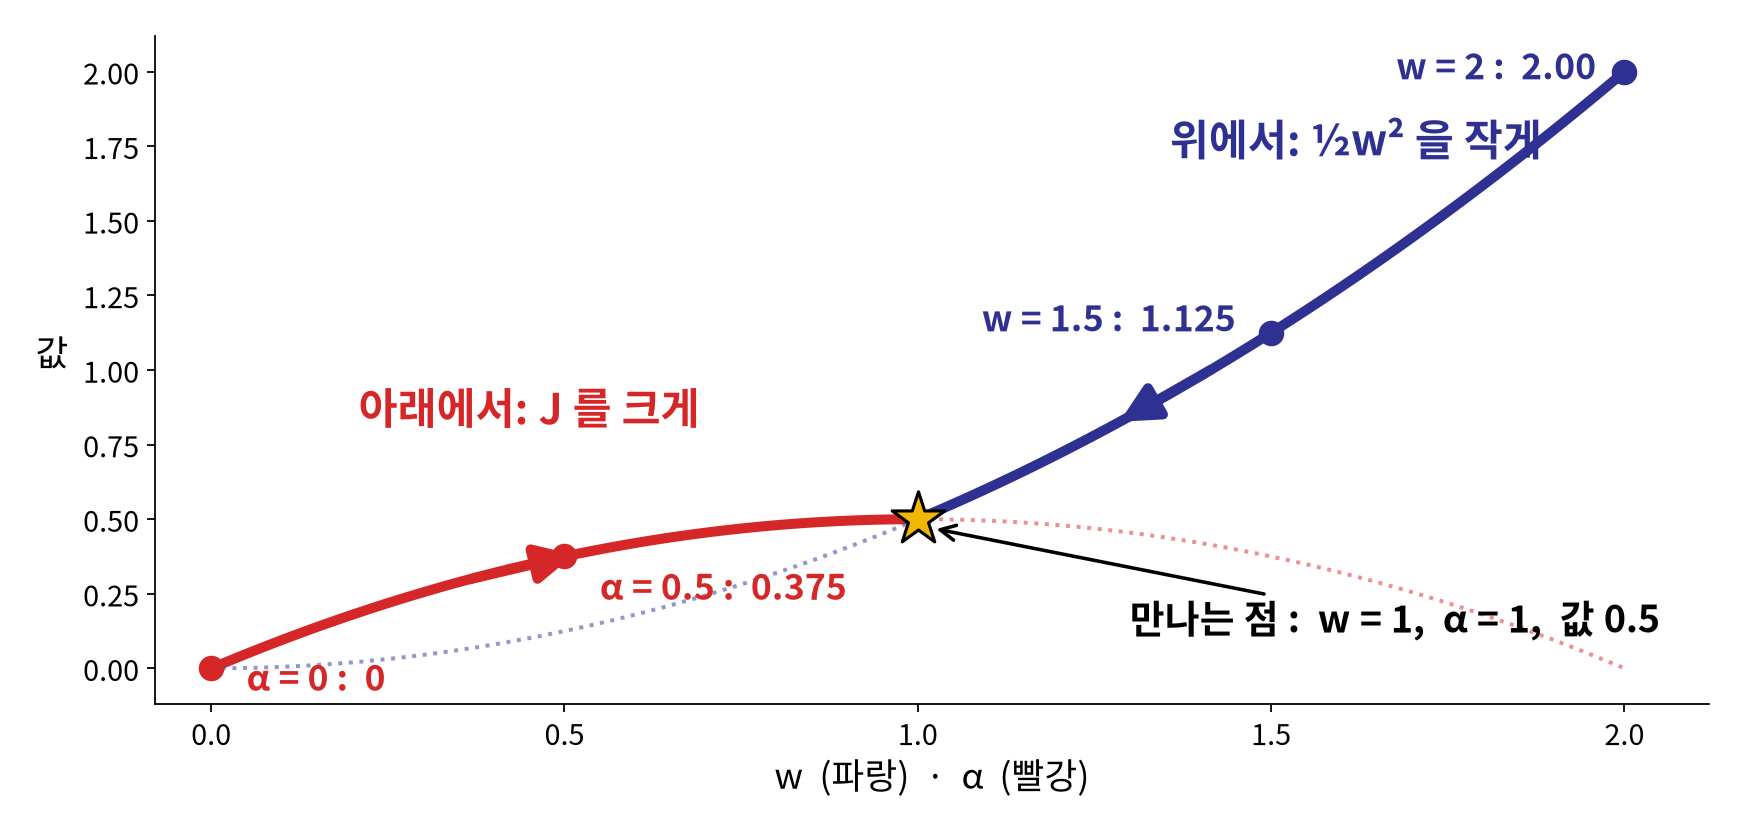
\includegraphics[width=0.76\linewidth]{kn_meet.png}\par\vskip0.3em
{\large 답은 \kb{파랑보다 위에 없고}, \kq{빨강보다 아래에 없다} \;$\to$\; 틈이 $0$ 이면 끝}\\[0.2em]
{\small\color{gray} 점 두 개 ($x = \pm 1$), 조건 $w \ge 1$ \qquad $J(\alpha) = 2\alpha - 2\alpha^2$ \; ($L$ 에 $w = 2\alpha$)}
\vfill
\note{방금 안장점의 두 곡선을 업다운 게임처럼 읽어 봅시다. 답을 양쪽에서 좁혀 가는 것입니다. 같은 작은 예입니다. 2분의 1 w 제곱을 가장 작게 하되 w는 1 이상이어야 합니다. 위쪽 파랑은 조건을 지키는 w를 하나 골라 값을 잰 것입니다. w가 2면 2입니다. 진짜 답은 가장 작은 값이니 2보다 클 수 없습니다. 아래쪽 빨강은 알파를 하나 골라 J를 잰 것입니다. 알파를 정하고 L이 가장 낮은 w, 즉 w가 2 알파인 곳의 값이 J이고, 2 알파 빼기 2 알파 제곱입니다. 알파가 0이면 0입니다. J는 어떤 알파를 골라도 파랑보다 클 수 없어서, 답은 이 값보다 작지 않습니다. 처음에는 답이 0과 2 사이라는 것만 알고, 틈이 2입니다. w를 1.5로 줄이고 알파를 0.25로 키우면 1.125와 0.375, 틈이 0.75로 좁아집니다. w가 1, 알파가 0.5이면 둘 다 0.5, 틈이 0입니다. 위에서도 아래에서도 더 갈 수 없으니 이것이 답입니다. 이렇게 파랑의 최소와 빨강의 최대가 같은 것을 쌍대성이라고 합니다. 점 20개에서도 두 값이 똑같이 1.11입니다. 그래서 w를 찾는 대신 알파를 키워도 같은 답에 닿습니다.}
\end{frame}

% --- sklearn 은
\begin{frame}[fragile]{sklearn 은: 같은 $J$ 를 SMO 로}
\vfill
\centering
{\large\begin{tabular}{rl}
푸는 문제 & 같은 $J$ 를 최대로\\
조건 & $\alpha_k \ge 0$, \quad $\sum_k \alpha_k y_k = 0$\\
방법 & \kb{SMO}: $\alpha$ \textbf{두 개씩} 골라 고치기를 반복 (LIBSVM)
\end{tabular}}\\[1em]
\begin{minipage}{0.82\linewidth}\small
\begin{verbatim}
m = SVC(kernel="linear", C=1e6).fit(X, y)   # hard margin = very large C
m.support_      # indices of the 3 support vectors
m.dual_coef_    # alpha_k * y_k :  -0.554  -0.554  1.108
m.intercept_    # b = 0.052
\end{verbatim}
\end{minipage}\\[0.5em]
{\normalsize 두 개씩인 이유: $\sum \alpha_k y_k = 0$ 을 지키려면 하나만 바꿀 수 없다}
\vfill
\note{실무에서 쓰는 sklearn의 SVC는 안에서 LIBSVM이라는 라이브러리를 쓰고, 방금 본 J를 풉니다. 라이브러리는 부호를 뒤집어 최소로 푸는데 같은 문제입니다. 조건은 알파가 0 이상이고, 알파 y의 합이 0입니다. 푸는 방법은 SMO, 알파를 두 개씩 골라 고치기를 반복합니다. 합이 0이라는 조건을 늘 지켜야 해서 알파 하나만 바꾸면 합이 깨지기 때문입니다. 두 개를 같이 바꾸면 합을 지키면서 J를 키울 수 있습니다. 앞에서 본 수업용 방법은 모든 알파를 조금씩 움직이고 b로 합을 점점 맞추는 것이라 방법은 다르지만 답은 같습니다. sklearn에는 하드 마진이 따로 없어서 C라는 값을 아주 크게 줍니다. C가 무엇인지는 뒤의 소프트 마진에서 배웁니다. 결과에서 support 속성은 서포트 벡터의 번호, dual coef는 알파 곱하기 y, intercept는 b입니다. 파란 두 점은 y가 마이너스 1이라 마이너스 0.554, 빨강은 1.108입니다.}
\end{frame}

% --- 참고: 라그랑주 함수
\begin{frame}{참고: 라그랑주 함수 (Lagrangian) 란}
\vfill
\centering
{\large 조건 있는 최소화: \; $\min_{\mathbf{w}} f(\mathbf{w})$, \; 조건 $g_k(\mathbf{w}) \ge 0$}\\[0.9em]
{\large 조건마다 \kb{벌의 크기 $\alpha_k \ge 0$} 를 붙여 \textbf{식 하나로}}\\[0.3em]
{\Large $\displaystyle L(\mathbf{w}, \boldsymbol{\alpha}) = f(\mathbf{w}) - \sum_k \alpha_k\, g_k(\mathbf{w})$ \qquad $\displaystyle \min_{\mathbf{w}}\ \max_{\boldsymbol{\alpha} \ge 0}\ L(\mathbf{w}, \boldsymbol{\alpha})$}\\[1em]
\renewcommand{\arraystretch}{1.35}
{\normalsize\begin{tabular}{c|c|c}
\textbf{$\mathbf{w}$ 가 조건을} & \textbf{$L$ 을 가장 크게 하는 $\alpha_k$} & \textbf{$\max_{\boldsymbol{\alpha}} L$}\\ \hline
\kq{어김} ($g_k < 0$) & 끝없이 크게 & $\infty$\\
\kb{지킴} ($g_k \ge 0$) & $\alpha_k g_k = 0$ 이 되게 & $f(\mathbf{w})$
\end{tabular}}\\[0.8em]
{\large 그래서 바깥의 $\min_{\mathbf{w}}$ 는 \textbf{조건을 지키는 $\mathbf{w}$ 중 $f$ 최소} = 원래 문제}\\[0.4em]
{\normalsize SVM: \; $f = \tfrac12\lVert\mathbf{w}\rVert^2$, \quad $g_k = y_k D(\mathbf{x}_k) - 1$}
\vfill
\note{라그랑주 함수가 무엇인지 먼저 일반적인 모양으로 봅시다. f를 가장 작게 하고 싶은데, 조건 g k가 0 이상이어야 합니다. 조건마다 0 이상인 숫자 알파 k를 붙여, f에서 알파 곱하기 g의 합을 뺀 식 하나를 만듭니다. 이것이 라그랑주 함수이고, 알파가 라그랑주 승수입니다. 그리고 안쪽에서 알파에 대해 가장 크게, 바깥에서 w에 대해 가장 작게 합니다. 표를 보면 왜 같은 문제인지 알 수 있습니다. w가 조건을 하나라도 어기면 g가 마이너스라서, 알파를 키울수록 L이 끝없이 커집니다. 조건을 모두 지키면 알파 곱하기 g를 빼면 L이 작아지기만 하니, 가장 큰 값은 그 곱이 0일 때, 즉 f 그대로입니다. 바깥의 최소화는 무한대인 w를 절대 고르지 않으니, 조건을 지키는 w 중에서 f가 가장 작은 것을 찾습니다. SVM에서는 f가 2분의 1 w 길이 제곱이고, g k는 y k D x k 빼기 1입니다. SVM처럼 볼록한 문제에서는 최소와 최대의 순서를 바꿔도 답이 같아서, 뒤에서는 w를 먼저 최소로 만들고 알파를 최대로 합니다.}
\end{frame}

% --- 라그랑주 함수
\begin{frame}{참고: 답은 $L$ 의 안장점}
\vfill
\centering
{\large 조건 ($y_k D(\mathbf{x}_k) \ge 1$) 마다 \kb{무게 $\alpha_k$} 를 붙여 \textbf{식 하나로}}\par\vspace{1.15cm}
{\large $L(\mathbf{w}, b, \boldsymbol{\alpha}) = \tikzmarknode{hw}{\tfrac{1}{2}\lVert\mathbf{w}\rVert^2} - \sum_{k=1}^{p} \tikzmarknode{al}{\alpha_k}\,\tikzmarknode{br}{\big[\,y_k D(\mathbf{x}_k) - 1\,\big]}$}\\[0.2em]
\begin{tikzpicture}[remember picture,overlay]
\node[bub,anchor=south east,font=\small] (c1) at ([xshift=0.15cm,yshift=0.45cm]hw.north) {줄이고 싶은 것: $\lVert\mathbf{w}\rVert$ 작게 = \textbf{넓은 길}};
\draw[bubarr] (c1.south east) -- (hw.north);
\node[bub,anchor=south west,font=\small] (c3) at ([xshift=-1.0cm,yshift=0.45cm]br.north) {점 $\mathbf{x}_k$ 의 \textbf{여유}: $0$ = 가장자리, $+$ = 길 밖};
\draw[bubarr] ([xshift=1.0cm]c3.south west) -- (br.north);
\node[bub,anchor=north,font=\small] (c2) at ([yshift=-0.45cm]al.south) {조건마다 붙인 \textbf{무게} = 점 $\mathbf{x}_k$ 가 \textbf{미는 힘}};
\draw[bubarr] (c2.north) -- (al.south);
\end{tikzpicture}\par\vspace{0.85cm}
{\large $\displaystyle\min_{\mathbf{w},\,b}\ \max_{\boldsymbol{\alpha} \ge 0}\ L(\mathbf{w}, b, \boldsymbol{\alpha})$ \;의 답 $=$ $L$ 의 \kb{안장점} (saddle point)}\\[0.5em]
{\large $L$ 이 $\mathbf{w}$ 에 대해서는 \textbf{최소}, \; $\boldsymbol{\alpha}$ ($\alpha_k \ge 0$) 에 대해서는 \kq{최대} 인 점}\\[0.3em]
{\large $L(\mathbf{w}^*, b^*, \textcolor{ksared}{\boldsymbol{\alpha}}) \;\le\; L(\mathbf{w}^*, b^*, \boldsymbol{\alpha}^*) \;\le\; L(\textcolor{ksablue}{\mathbf{w}}, b^*, \boldsymbol{\alpha}^*)$}\\[0.4em]
{\normalsize $\alpha_k$ = \kb{라그랑주 승수} (Lagrange multiplier)}
\vfill
\note{라그랑주 방법은 조건이 붙은 문제를 식 하나로 바꾸는 방법입니다. 조건마다 숫자 하나, 알파 k를 붙여서 조건을 식 안으로 넣습니다. 앞의 2분의 1 w 길이 제곱은 줄이고 싶은 것, 넓은 길입니다. 대괄호 안, y k D x k 빼기 1은 점 k의 여유입니다. 0이면 길 가장자리, 플러스면 길 밖에 여유가 있고, 마이너스면 조건을 어긴 것입니다. 알파는 그 조건에 거는 무게이고, 뒤의 역학 비유로는 점 x k가 경계를 미는 힘입니다. 알파는 0 이상이고, 라그랑주 승수, 또는 Kuhn Tucker 계수라고 부릅니다. 원 논문의 식 14입니다. 답은 이 L이 w와 b에 대해서는 가장 작고, 알파에 대해서는 가장 큰 곳, 안장점입니다. 앞의 2분의 1은 미분했을 때 식이 깔끔해지라고 붙인 것이고, 논문도 답은 바뀌지 않는다고 적습니다. 그래서 앞의 최소화 문제를 푸는 것은 이 L의 안장점을 찾는 것과 같습니다. 원 논문의 문장 그대로, 안장점은 L이 w에 대해서는 가장 작고, 0 이상인 알파에 대해서는 가장 큰 점입니다. 크기를 말하는 것이 아니라 L의 값이 그렇다는 뜻입니다. 왜 알파는 크게 할까요. 어떤 점이 조건을 어기면 여유가 마이너스라서, 알파를 키울수록 L이 끝없이 커집니다. 그러니 w가 L을 작게 하려면 조건을 어길 수 없습니다. 조건을 다 지키면 L의 최댓값은 2분의 1 w 길이 제곱이 됩니다. 한 방향으로는 골짜기, 다른 방향으로는 봉우리라서 말안장 모양, 안장점이라고 부릅니다. b는 논문에서 따로 정하는데, 뒤에서 보겠습니다. 수식으로 쓰면 아래 한 줄입니다. 답 w 별, b 별에서 알파를 아무리 바꿔도 L은 더 커지지 않고, 답 알파 별에서 w를 아무리 바꿔도 L은 더 작아지지 않습니다.}
\end{frame}

% --- SVM 에서 왜 같은 문제인가
\begin{frame}{SVM 에서 보면: 왜 같은 문제인가}
\vfill
\centering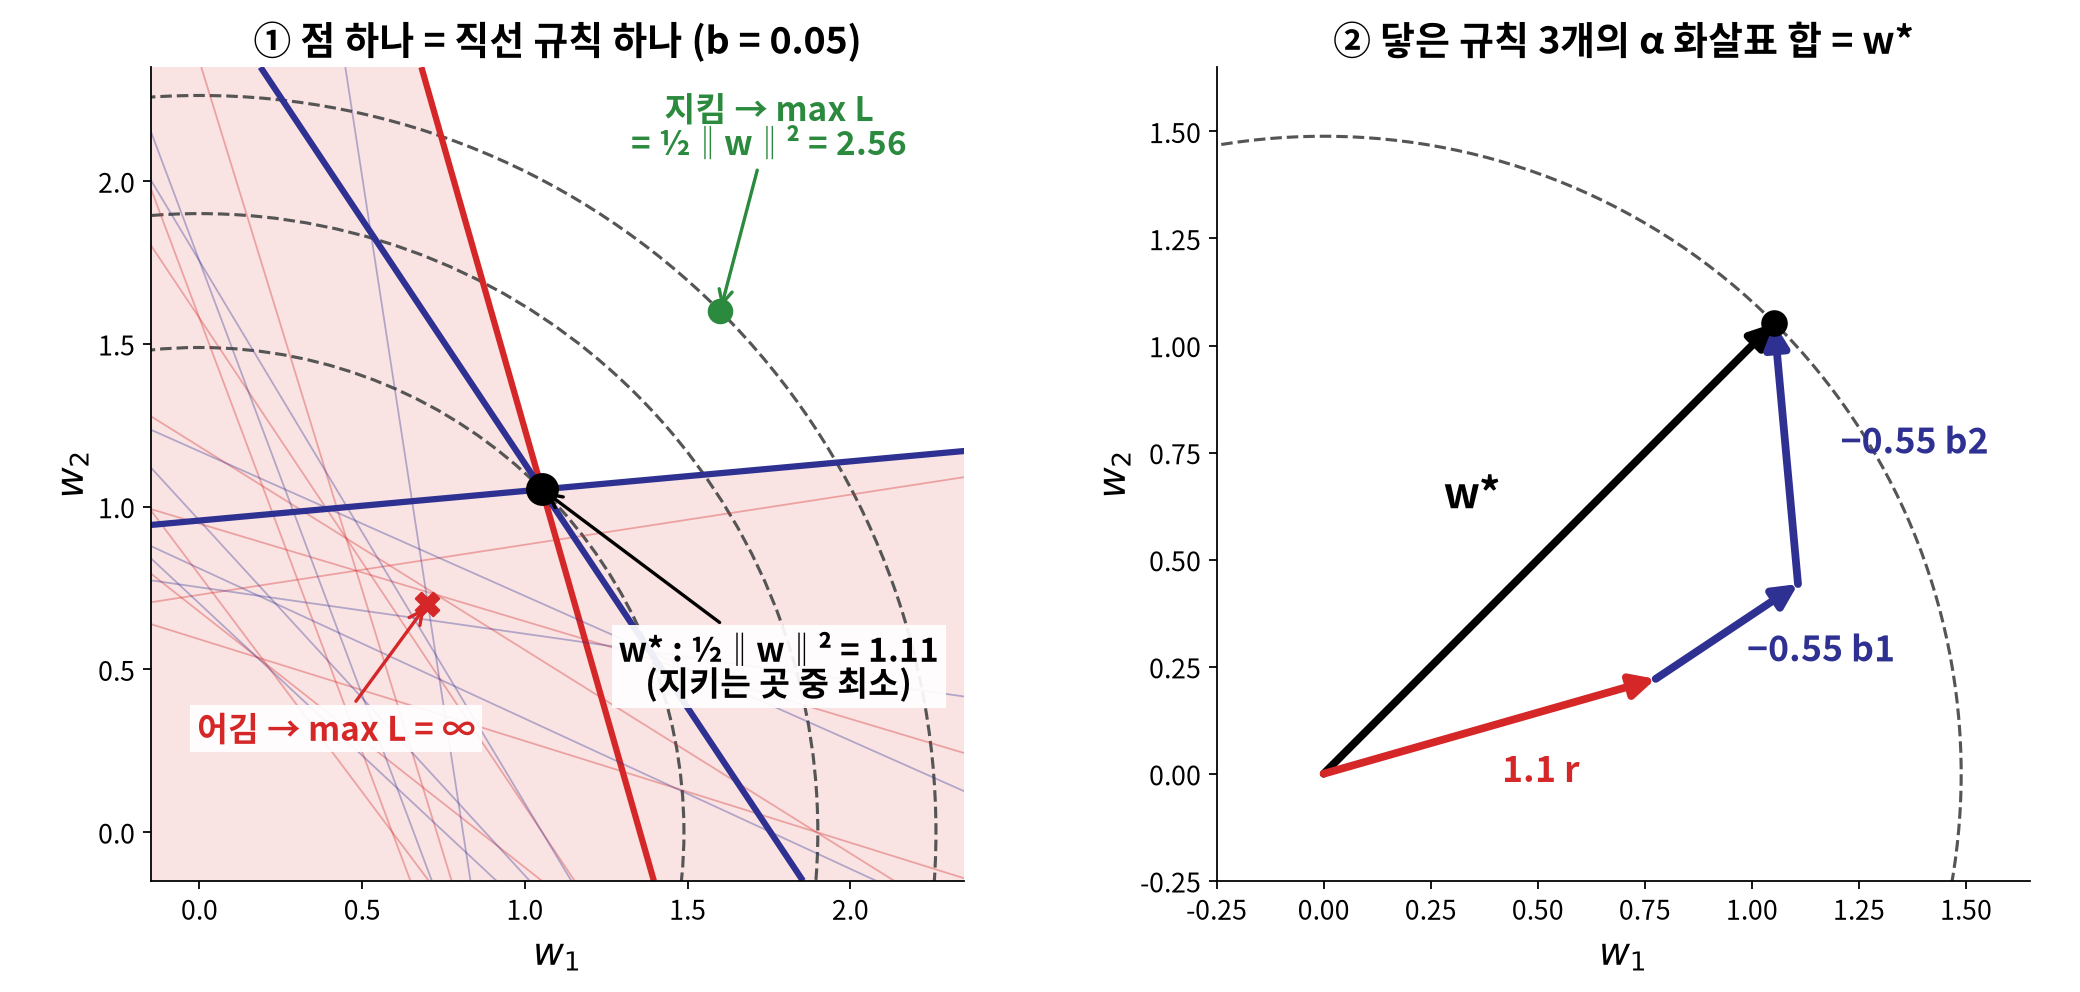
\includegraphics[width=0.78\linewidth]{kn_equiv.png}\par\vskip0.3em
{\large $\displaystyle \min_{\mathbf{w}} \max_{\boldsymbol{\alpha} \ge 0} L$ \;=\; \kq{빨간 곳은 $\infty$ 라 못 고른다} \;$\to$\; \textbf{지키는 곳에서 $\tfrac12\lVert\mathbf{w}\rVert^2$ 최소}}
\vfill
\note{점 20개로 왜 두 문제가 같은지 그려 봅시다. 가로축이 w1, 세로축이 w2이고, b는 답의 값 0.05로 고정합니다. 이 평면의 점 하나가 w 하나, 즉 경계 하나의 방향과 크기입니다. 데이터 점 하나는 y k D x k가 1 이상이라는 규칙 하나이고, 평면에서는 직선 하나입니다. 직선이 20개 있고, 20개를 모두 지키는 곳이 흰 부분입니다. 빨간 곳은 규칙을 하나라도 어긴 w입니다. 거기서는 어긴 점의 알파를 키우면 L이 끝없이 커지니 max L이 무한대입니다. 흰 곳에서는 알파 곱하기 여유를 빼면 작아지기만 하니, 가장 큰 값은 2분의 1 w 길이 제곱입니다. 바깥에서 w를 골라 최소로 하면 무한대인 곳은 절대 안 고르니, 흰 곳에서 원점에 가장 가까운 점, 검은 점이 답입니다. 원래 문제와 똑같습니다. 점선 원은 2분의 1 w 길이 제곱이 같은 곳입니다. 오른쪽 그림에서, 검은 점에 닿아 있는 직선은 3개뿐입니다. 이 3개 점의 알파 곱하기 라벨 곱하기 위치를 화살표로 이으면 정확히 w 별이 됩니다. 나머지 17개는 닿지 않아 알파가 0입니다.}
\end{frame}

% --- 고무줄 만화
\begin{frame}{참고: 점 6개로 보는 고무줄 당기기}
\vfill
\centering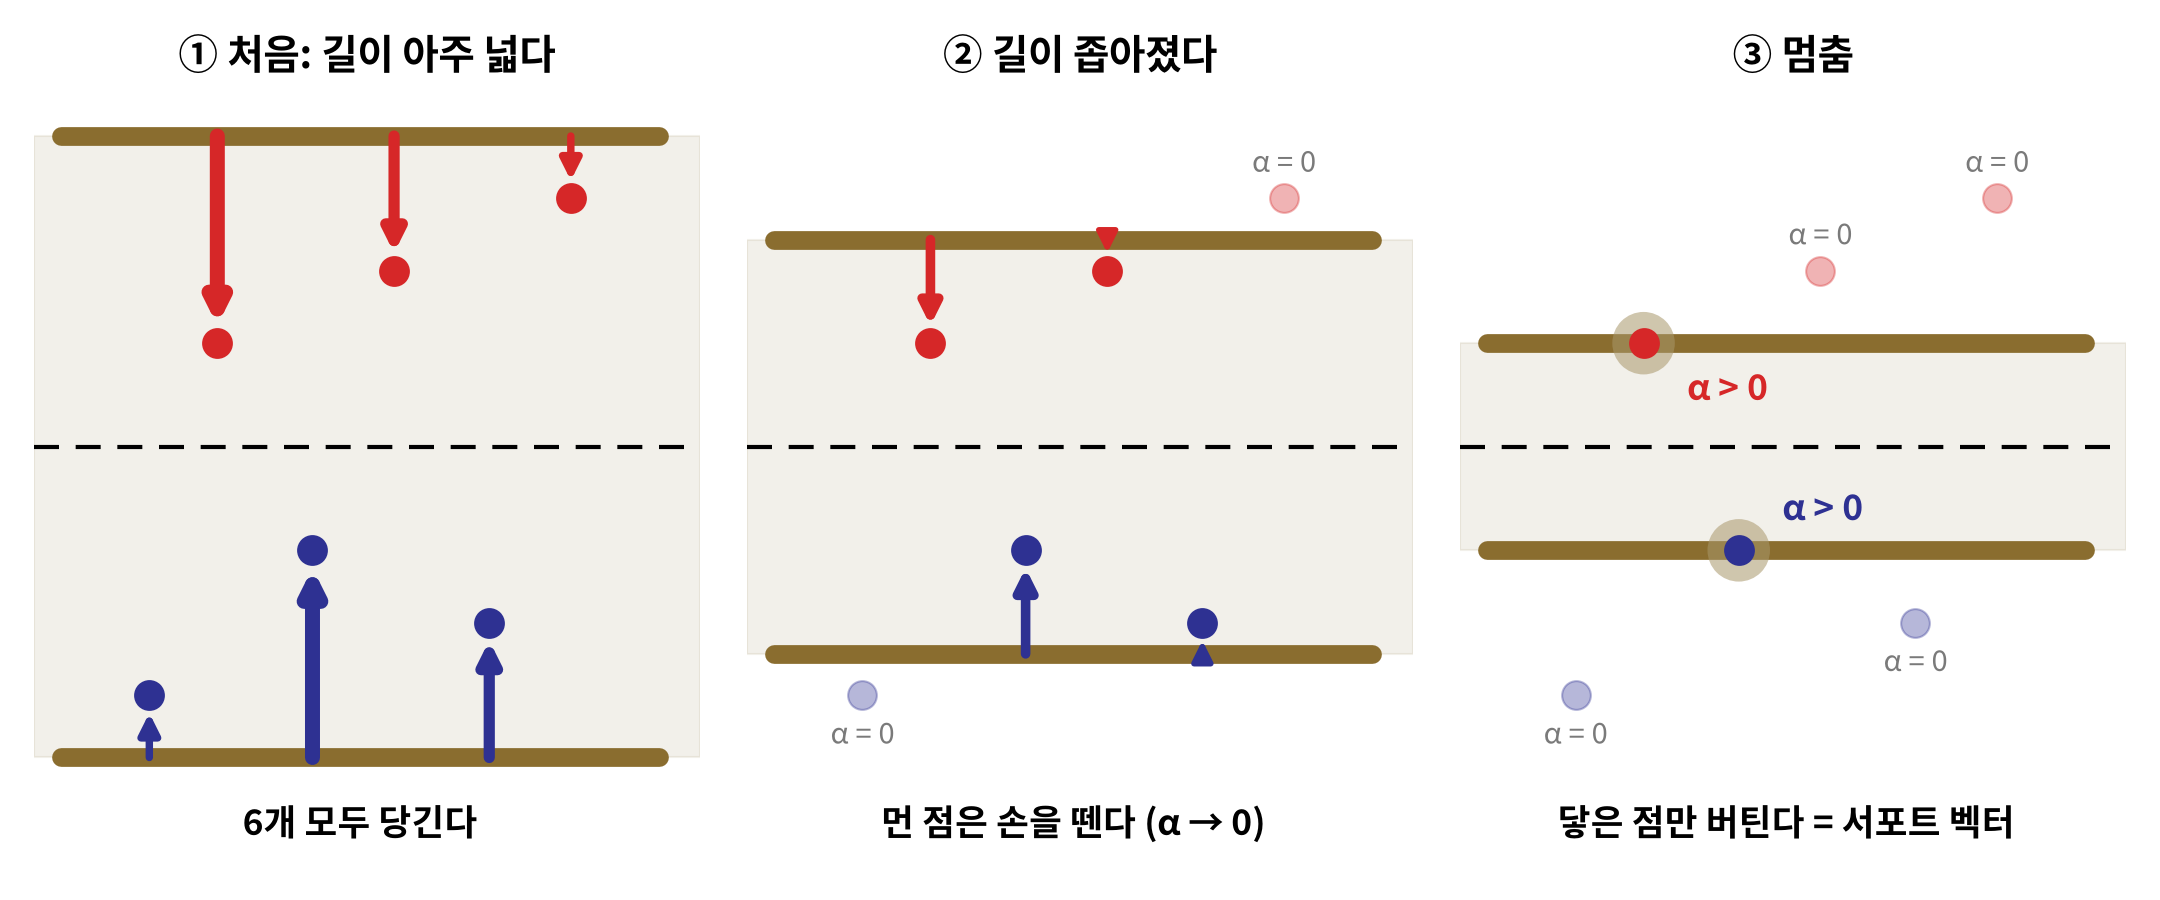
\includegraphics[width=0.85\linewidth]{kn_pull.png}\par\vskip0.4em
{\large 길 \textbf{안}의 점은 가장자리를 \kq{당긴다} ($\alpha \uparrow$) \qquad 길 \textbf{밖}의 점은 \kb{놓는다} ($\alpha \downarrow 0$)}
\vfill
\note{학습이 왜 서포트 벡터만 남기는지 고무줄로 생각해 봅시다. 가운데 점선이 경계이고, 갈색 막대 두 개가 길의 가장자리입니다. 모든 점은 길 밖에 있고 싶어 합니다. 길 안에 있는 점은 가장자리에 고무줄을 걸어 자기 쪽으로 당깁니다. 길 안으로 깊이 들어와 있을수록 세게 당기고, 당기는 동안 알파가 커집니다. 처음에는 w가 0이라 길이 아주 넓어서 모든 점이 당깁니다. 당기는 힘에 길이 좁아지면, 멀리 있는 점은 길 밖이 됩니다. 길 밖의 점은 더 당길 이유가 없어서 알파가 줄고, 0에서 멈춥니다. 마지막에는 가장 가까운 점이 가장자리에 딱 닿습니다. 길은 넓을수록 좋아서 더 좁아지지는 않고, 닿은 점이 더 넓어지지 못하게 버팁니다. 그래서 알파가 0보다 큰 점은 닿은 점, 서포트 벡터뿐입니다. 식으로는 값이 1보다 작으면 알파를 키우고, 1보다 크면 줄이는 한 줄이 전부입니다. 그림의 알파와 길 폭은, 높이만 다른 점 6개를 실제로 학습한 숫자입니다. 좌우 위치는 그림을 위한 것입니다. 처음 세 걸음에는 모두 0.02에서 0.03이고, 40걸음에는 가까운 두 점이 0.21로 크고, 중간 두 점은 길 밖으로 나가 0.07로 줄어드는 중이며, 먼 두 점은 이미 0입니다. 300걸음에는 가까운 두 점만 0.50입니다. 점 20개도 똑같이 움직입니다.}
\end{frame}

% --- 벌금 게임 그림
\begin{frame}{참고: 벌금 게임 ($\tfrac12 w^2$ 최소, 규칙 $w \ge 1$)}
\vfill
\centering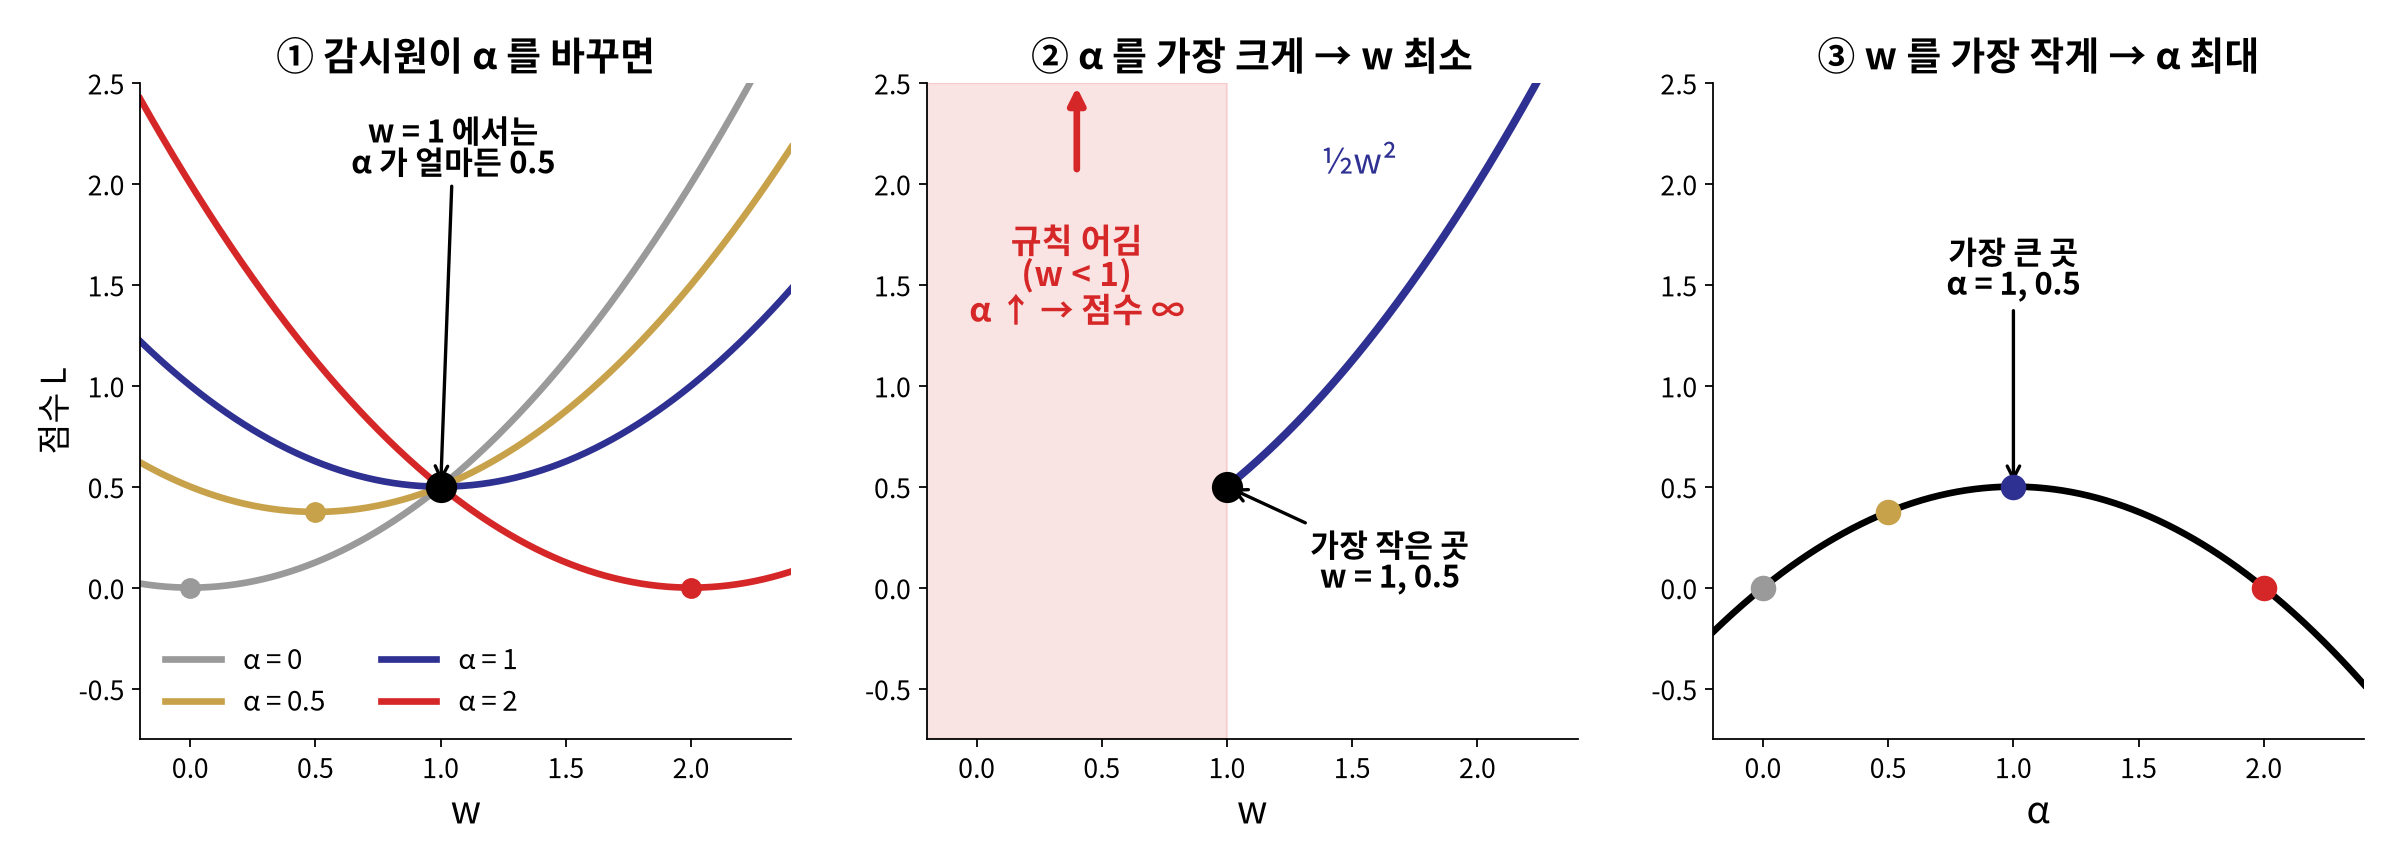
\includegraphics[width=0.94\linewidth]{kn_penalty.png}\par\vskip0.3em
{\large $L(w, \alpha) = \tfrac12 w^2 - \alpha\,(w - 1)$ \qquad 나는 $w$ 로 \kb{작게}, 감시원은 $\alpha$ 로 \kq{크게}}\\[0.4em]
{\large 답: $w = 1$, \; $\alpha = 1$, \; $L = 0.5$}
\vfill
\note{라그랑주 함수를 벌금 게임으로 그려 봅시다. 나는 2분의 1 w 제곱을 작게 하고 싶고, 규칙은 w가 1 이상입니다. 감시원은 벌금 단가 알파를 정합니다. 점수 L은 2분의 1 w 제곱 빼기 알파 곱하기 w 빼기 1이고, 나는 작게, 감시원은 크게 하려 합니다. 첫째 그림은 알파를 0, 0.5, 1, 2로 바꾼 곡선입니다. w가 1인 곳에서는 벌금 항이 0이라, 네 곡선이 모두 0.5를 지납니다. 둘째 그림은 감시원이 먼저 최선을 다한 것입니다. w가 1보다 작으면 알파를 키울수록 점수가 끝없이 커지고, 1 이상이면 알파 0이 가장 커서 2분의 1 w 제곱만 남습니다. 그래서 내가 고를 수 있는 가장 작은 곳은 w가 1입니다. 원래 문제와 같습니다. 셋째 그림은 순서를 바꾼 것입니다. 알파가 정해지면 나는 점수가 가장 작은 w, 즉 w는 알파를 고릅니다. 그 점수를 알파마다 찍으면 산 모양이고, 알파가 1에서 가장 높습니다. 값은 똑같이 0.5입니다. 이 셋째 그림이 본편에서 만든 J입니다.}
\end{frame}

% --- 소프트 마진 학습 한 걸음
\begin{frame}{소프트 마진의 학습 한 걸음: 길 안의 점들이 다 같이 민다}
\vfill
\centering
\renewcommand{\arraystretch}{1.75}
{\small\begin{tabular}{c|l|l}
 & \textbf{하드 마진} ($\lVert\mathbf{w}\rVert = 1$) & \textbf{소프트 마진} (가장자리 $D(\mathbf{x}) = \pm 1$)\\ \hline
\textbf{1.} 값 재기 & \multicolumn{2}{c}{점마다 $y_k D(\mathbf{x}_k)$ \; (같다)}\\ \hline
\textbf{2.} 미는 점 & 값이 \kq{가장 작은 점 하나} $k$ & 값이 1 보다 작은 점 \kb{모두} $V$\\
 & $\mathbf{w}' = \mathbf{w} + \eta\, y_k \mathbf{x}_k$ & $\mathbf{w}' = \mathbf{w} - \eta\,\big(\mathbf{w} - C \sum_{k\in V} y_k \mathbf{x}_k\big)$\\
 & $b' = b + \eta\, y_k$ & $b' = b + \eta\, C \sum_{k\in V} y_k$\\ \hline
\textbf{3.} 길 폭 & $\mathbf{w} \leftarrow \mathbf{w}'/\lVert\mathbf{w}'\rVert$, \;$M$ = 가장 작은 값 & 나누지 않는다, \;$M = 1/\lVert\mathbf{w}\rVert$
\end{tabular}}\\[0.6em]
{\normalsize $-\eta\,\mathbf{w}$: $\mathbf{w}$ 가 줄어 길을 \kb{넓힌다} \quad 길 안 점들의 $C$ 배 밀기: 길을 \kq{좁힌다} \quad 학습률 $\eta = 1/\text{걸음}$}\\[0.3em]
{\small 이상치 포함 21개, $C = 3$: $\mathbf{w} = (1.05, 1.05)$, $b = 0.05$, $M = 0.67$ \;= sklearn 결과와 같은 선}
\vfill
\note{소프트 마진일 때 학습이 어떻게 바뀌는지 봅시다. 왼쪽이 하드 마진, 오른쪽이 소프트 마진입니다. 1번은 같고, 2번과 3번이 다릅니다. 2번이 핵심입니다. 하드 마진에서는 값이 가장 작은 점 하나 k만 밀었습니다. 소프트 마진에서는 값이 1보다 작은 점들, 즉 길 가장자리를 넘어 길 안에 들어왔거나 반대편으로 넘어간 점들이 모두 다 같이 밉니다. 각자 자기 y x에 C를 곱한 만큼 w를 밀고, b에는 C 곱하기 y를 더합니다. 여기에 하나가 더 붙습니다. 매 걸음 w에서 학습률 곱하기 w를 빼서 w를 조금 줄입니다. 3번, 소프트 마진은 가장 가까운 값을 1로 두는 기준이라 w를 길이로 나누지 않고, 길 폭 M은 1 나누기 w의 길이입니다. 그래서 w를 줄이는 것이 곧 길을 넓히는 것입니다. 정리하면 두 힘이 겨룹니다. 빼기 에타 w는 길을 넓히고, 길 안 점들의 C배 밀기는 그 점들을 길 밖으로 내보내려고 w를 키워 길을 좁힙니다. C가 크면 미는 힘이 세서 좁은 길, 작으면 넓은 길이 됩니다. 이것이 앞 식, 2분의 1 w 길이 제곱 더하기 C 곱하기 크사이의 합을 한 걸음씩 줄이는 방법이고, 학습률은 1 나누기 걸음 수입니다. 이상치가 있는 21개로 C 3으로 2만 걸음 돌리면 w가 1.05, 1.05, b가 0.05, M이 0.67로, sklearn과 같은 선이 나옵니다.}
\end{frame}

% --- 소프트 마진 숫자로
\begin{frame}{소프트 마진 학습을 숫자로 따라가 보면 ($C = 3$)}
\vfill
\centering
\renewcommand{\arraystretch}{1.1}
{\large\begin{tabular}{r|rrr|r|l}
걸음 뒤 & $w_1$ & $w_2$ & $b$ & $M$ & 다음에 미는 점 $V$\\ \hline
0 & 0 & 0 & 0 & -- & 21개 모두 \; (선 없음, 값 모두 0)\\
1 & $48.90$ & $52.80$ & $3.00$ & 0.01 & 이상치 \textcolor{ksared}{$(-0.2, -0.6)$} 1개\\
5 & $9.30$ & $9.12$ & $6.85$ & 0.08 & 이상치 1개\\
10 & $5.07$ & $5.82$ & $5.15$ & 0.13 & 3개 (이상치 + \textcolor{ksablue}{파랑 2})\\
20 & $3.00$ & $4.10$ & $3.31$ & 0.20 & 3개\\
50 & $1.81$ & $2.53$ & $1.55$ & 0.32 & 2개 (이상치 + \textcolor{ksablue}{파랑 1})\\
100 & $1.44$ & $1.66$ & $0.68$ & 0.46 & 2개\\
200 & $1.11$ & $1.13$ & $0.11$ & 0.63 & 이상치 1개\\
2만 & $1.05$ & $1.05$ & $0.05$ & \kb{0.67} & 3개 (이상치 + \textcolor{ksablue}{파랑 2}) $\to$ 거의 멈춤\\ \hline
sklearn 답 & $1.05$ & $1.05$ & $0.05$ & 0.67 &
\end{tabular}}
\vfill
\note{이상치가 들어간 21개로 C 3인 소프트 마진 학습을 실제로 돌린 숫자입니다. 각 줄은 그만큼 걸은 뒤의 숫자와 그 다음 걸음에 미는 점들입니다. 출발할 때는 w, b가 모두 0이고 모든 점의 값이 0이라 1보다 작으니, 21개가 모두 C배로 밀어 첫 선이 생깁니다. 첫 걸음의 학습률이 1이라 w가 48.9, 52.8로 아주 크고, 길 폭 M은 0.01, 거의 선뿐입니다. 이때 길 안에 든 점은 파랑 무리 속의 빨간 이상치 하나입니다. 그다음부터 빼기 에타 w가 w를 줄여 길이 넓어지고, 이상치는 혼자 밀어 b를 키웁니다. 선이 파랑 쪽으로 밀려 갑니다. 10걸음 뒤 M은 0.13이고, 길이 넓어지면서 파란 점 둘이 길 안으로 들어와 미는 점이 3개가 됩니다. 이제 파란 점들이 b를 반대로 끌어당겨 b가 5.15에서 0.68, 0.11로 내려옵니다. 200걸음 뒤에는 M이 0.63으로 거의 답에 닿고, 2만 걸음 뒤 w는 1.05, 1.05, b는 0.05, M은 0.67로 sklearn이 낸 답과 같습니다.}
\end{frame}

% --- 소프트 마진 걸음별
\begin{frame}{소프트 마진: 길이 넓어지다 3개가 길 안에서 멈춘다 (1/3)}
\vfill
\centering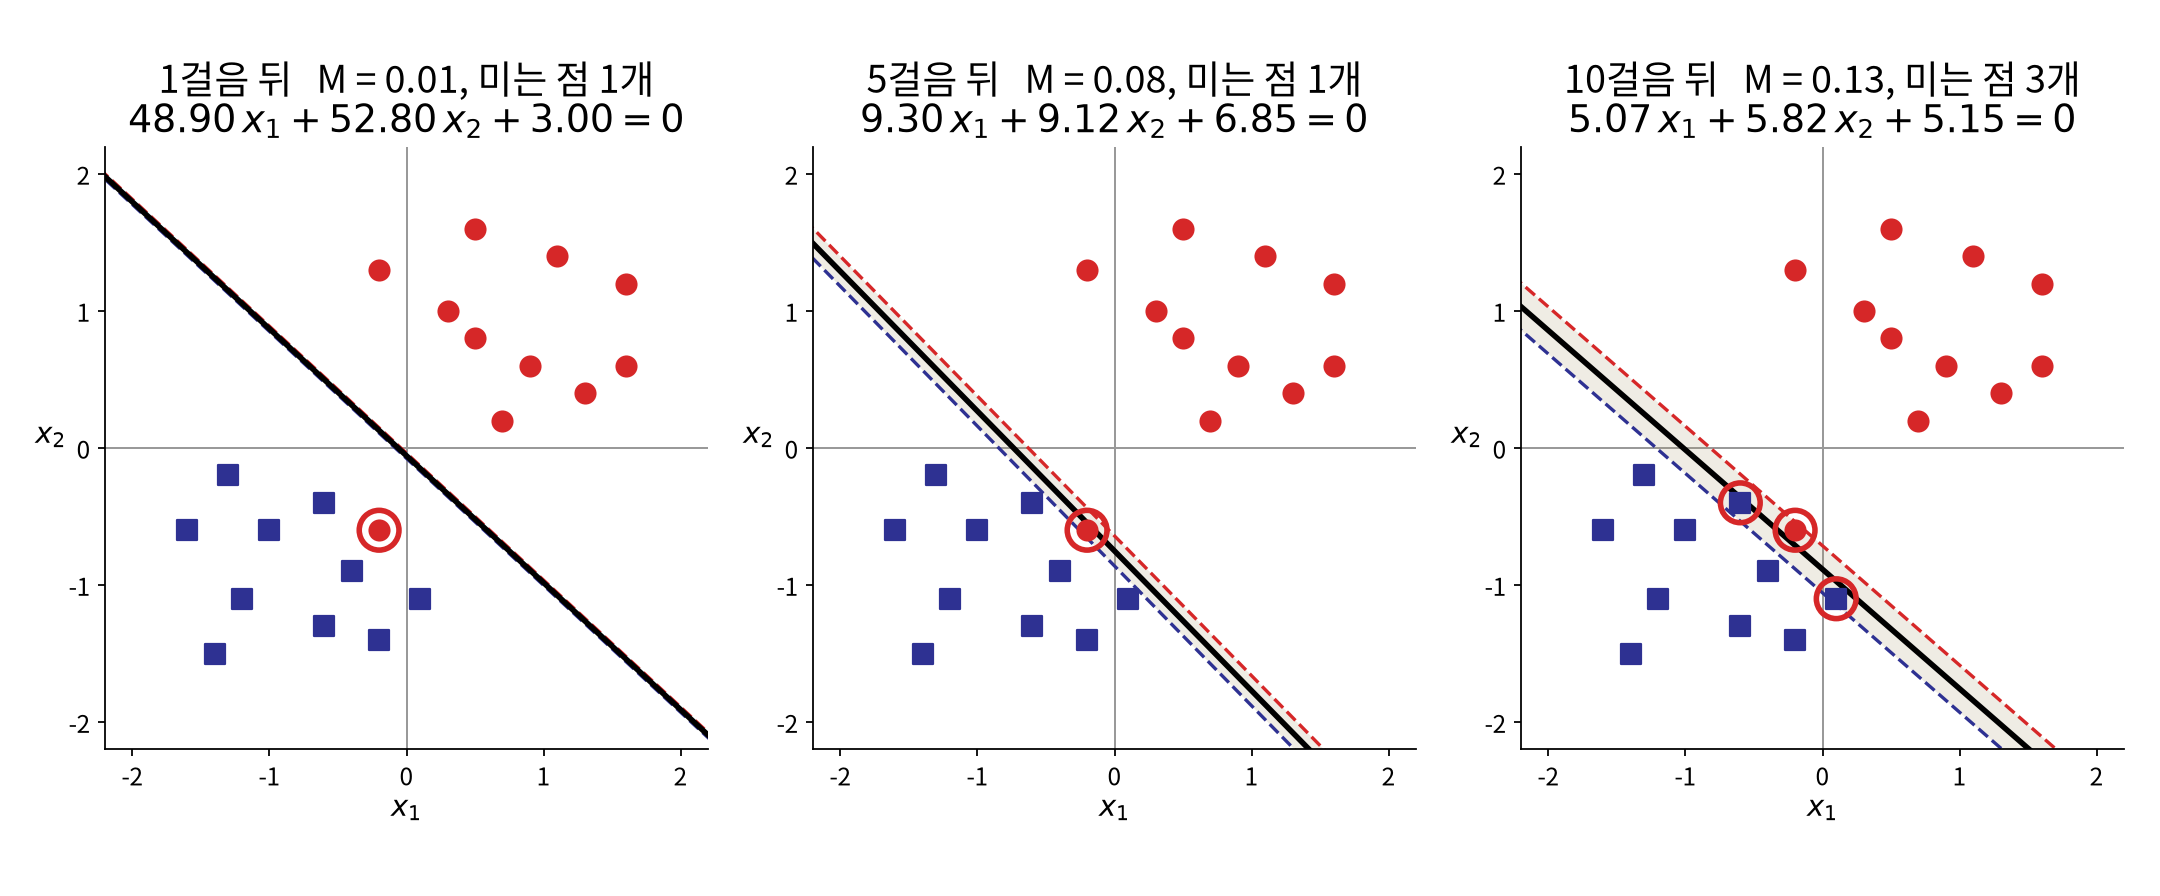
\includegraphics[width=0.95\linewidth]{sv_soft9_1.png}\par\vskip0.2em
{\large 첫 걸음: 21개가 $C$ 배로 밀어 $\mathbf{w}$ 가 크다 (\kq{좁은 길}) $\to$ $-\eta\,\mathbf{w}$ 로 줄며 길이 넓어진다}
\vfill
\note{빨간 동그라미가 그 걸음에 미는 점, 길 안이나 반대편에 있는 점입니다. 1걸음 뒤 M은 0.01이라 길이 거의 없고 경계선만 보입니다. 길 안에 든 점은 파랑 무리 속의 빨간 이상치 하나입니다. 매 걸음 w가 줄어 5걸음 뒤 M은 0.08, 10걸음 뒤 0.13으로 길이 넓어지고, 이상치가 자기 쪽으로 선을 밀어 선이 파랑 쪽으로 내려갑니다. 10걸음 뒤에는 파란 점 둘이 길 안에 들어왔습니다.}
\end{frame}

\begin{frame}{소프트 마진: 길이 넓어지다 3개가 길 안에서 멈춘다 (2/3)}
\vfill
\centering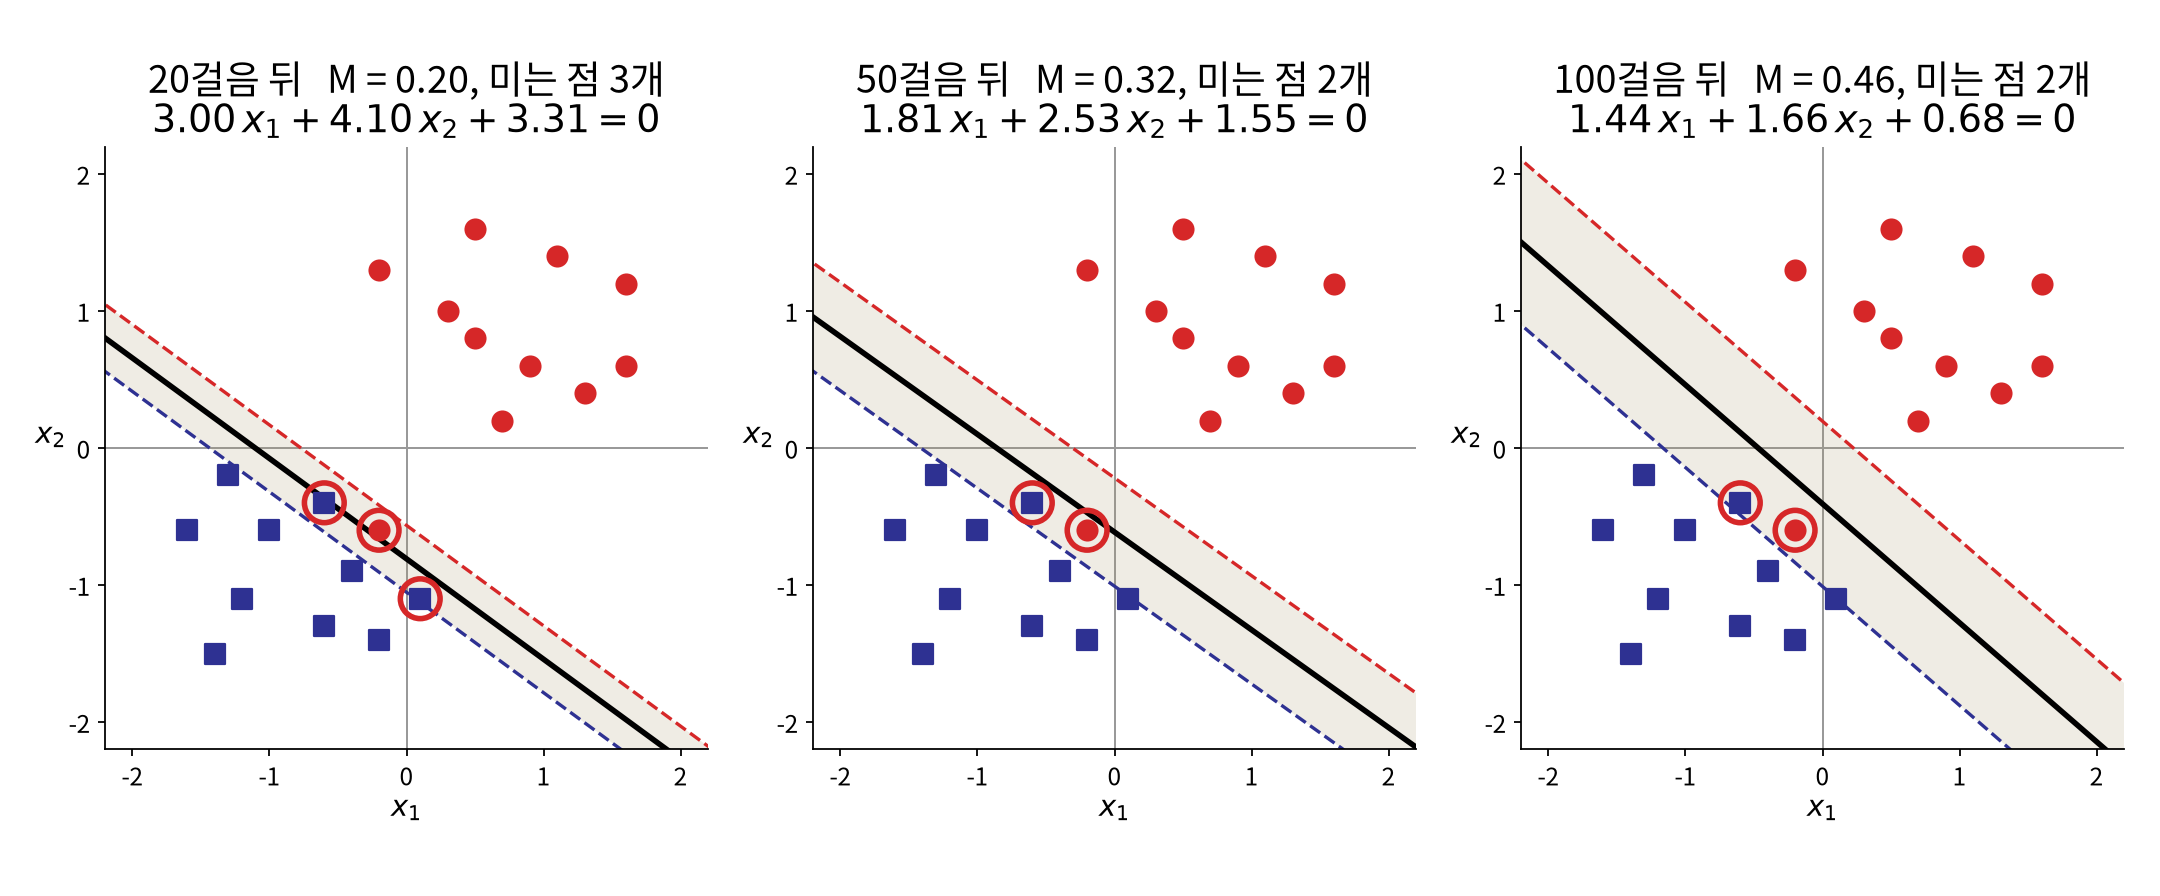
\includegraphics[width=0.95\linewidth]{sv_soft9_2.png}\par\vskip0.2em
{\large 길이 넓어지며 \textcolor{ksablue}{파란 점}이 길 안으로 $\to$ 같이 밀어 $b$ 가 돌아온다}
\vfill
\note{20걸음 뒤 M은 0.20이고, 파란 점 마이너스 0.6, 마이너스 0.4와 0.1, 마이너스 1.1이 길 안에서 이상치와 함께 밉니다. 파란 점 둘은 선을 빨강 쪽으로 밀어 b를 내립니다. 50걸음 뒤 b는 1.55, M은 0.32, 100걸음 뒤 b는 0.68, M은 0.46입니다.}
\end{frame}

\begin{frame}{소프트 마진: 길이 넓어지다 3개가 길 안에서 멈춘다 (3/3)}
\vfill
\centering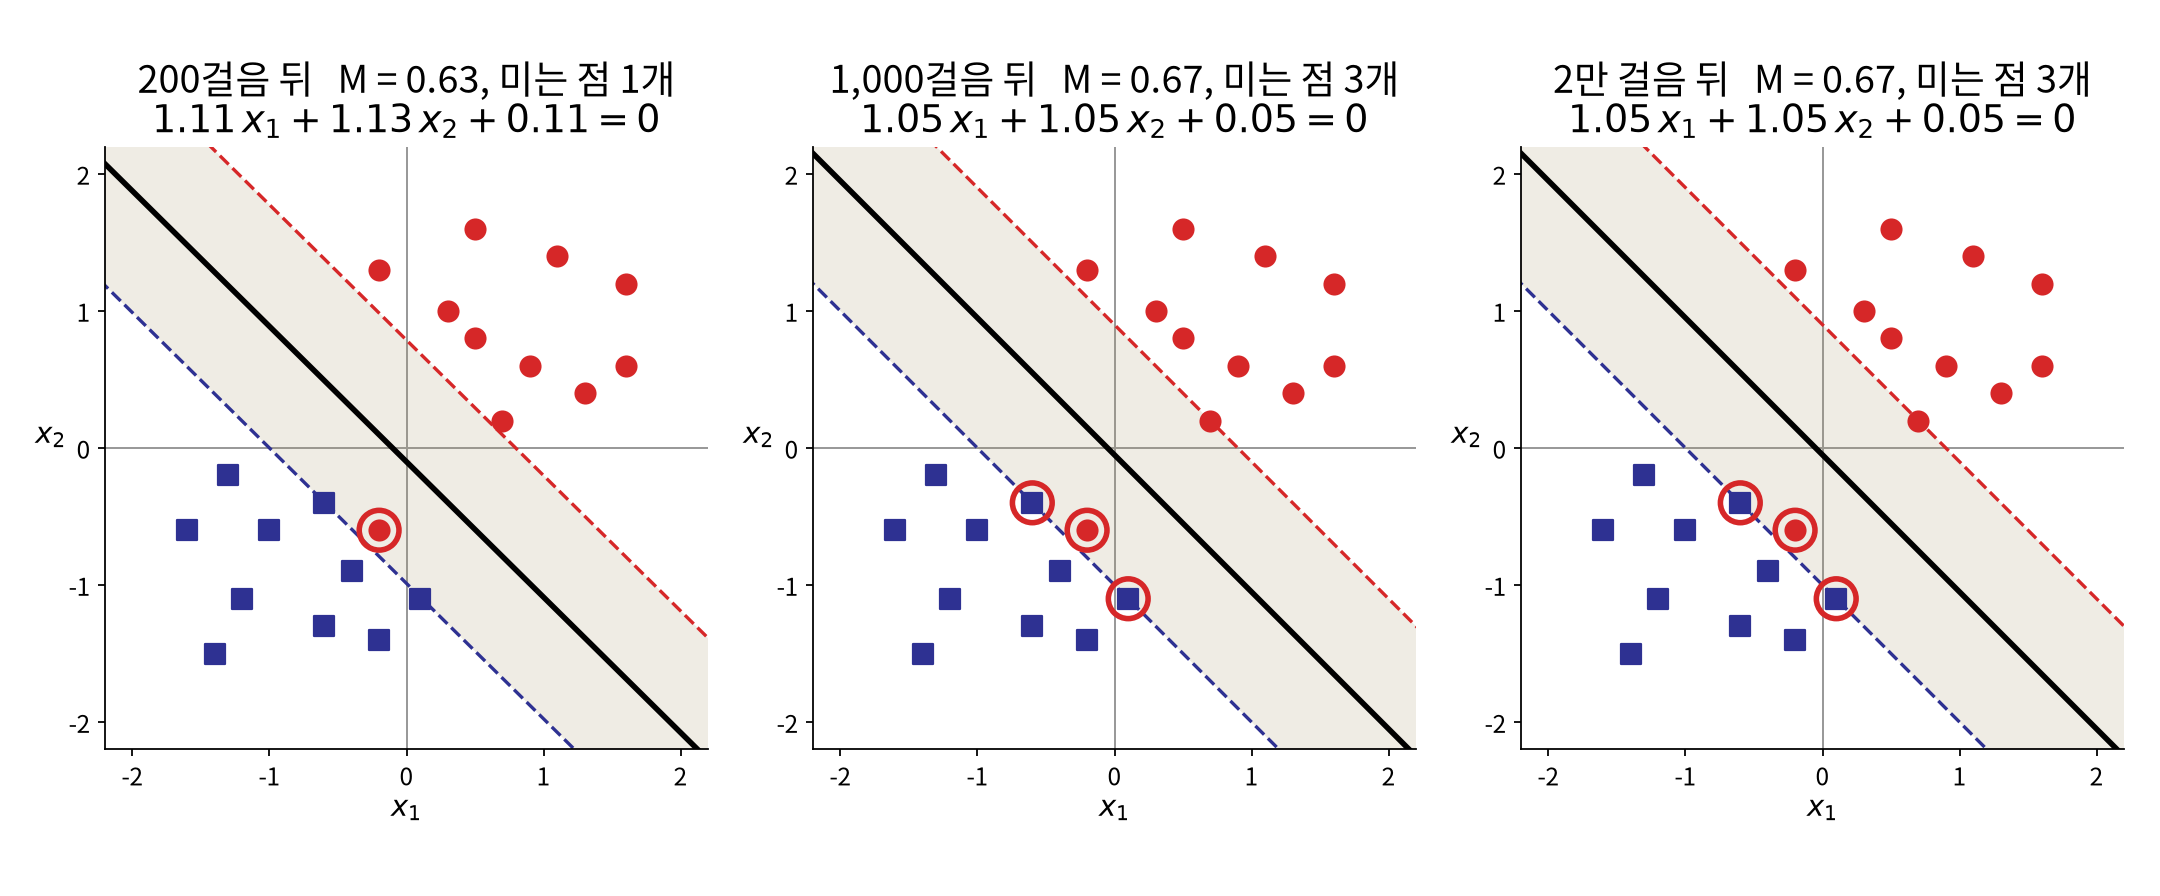
\includegraphics[width=0.76\linewidth]{sv_soft9_3.png}\par\vskip0.1em
{\large 넓히기 ($-\eta\,\mathbf{w}$) = 좁히기 (길 안 점들의 $C$ 배 밀기) $\to$ \kb{$M = 0.67$} 에서 멈춘다}\\[0.2em]
{\normalsize 가장자리 점이 들락날락 $\to$ $|V|$ 가 흔들 \;(흔들림 폭은 $\eta$ 따라 줄어든다)}
\vfill
\note{200걸음 뒤에는 거의 답과 같은 선이고 M은 0.63입니다. 1000걸음 뒤에는 1.05 x1 더하기 1.05 x2 더하기 0.05 = 0, 답과 같은 선이고 M은 0.67입니다. 이때 두 힘이 맞습니다. 빼기 에타 w가 길을 넓히려는 힘과, 길 안의 점들이 C배로 밀어 길을 좁히려는 힘이 같아져서 w가 더 이상 줄지도 늘지도 않습니다. 그런데 미는 점의 수는 딱 멈춰 있지 않고 오갑니다. 파란 두 점은 가장자리에 딱 걸쳐 있어서, 선이 아주 조금 움직이면 다음 걸음에 길 안으로 세어지기도 하고 바깥으로 세어지기도 합니다. 그래서 미는 점 수가 1개에서 3개 사이를 오가고, 그만큼 w와 b가 앞뒤로 아주 조금씩 떨립니다. 학습률이 1 나누기 걸음이라 걸음이 갈수록 떨림 폭이 줄어듭니다. 업데이트는 끝까지 계속되지만, 서로 상쇄되는 방향으로 오가며 폭이 점점 작아지는 것이 수렴입니다. 2만 걸음 뒤까지 선은 그대로이고 sklearn 답과 같습니다. 이상치는 길 반대편에 남아 틀린 채로 두고, 대신 넓은 길을 얻은 것입니다.}
\end{frame}

% --- Appendix: ISL 의 꼴
\begin{frame}{Appendix: ISL 교과서는 소프트 마진을 예산 $B$ 로 쓴다}
\vfill
\centering
\renewcommand{\arraystretch}{1.7}
{\small\begin{tabular}{l|l}
\textbf{이 덱} (Cortes · Vapnik) & $\min\; \tfrac12\lVert\mathbf{w}\rVert^2 + C\sum\xi_k$, \; $y_k D(\mathbf{x}_k) \ge 1 - \xi_k$\\
\textbf{ISL} (예산 $B$) & $\max\; M$, \; $\lVert\mathbf{w}\rVert = 1$, \; $y_k D(\mathbf{x}_k) \ge M(1 - \xi_k)$, \; $\sum\xi_k \le B$
\end{tabular}}\\[0.6em]
\renewcommand{\arraystretch}{1.4}
{\large\begin{tabular}{c|c|c|c}
$C$ & $M$ & $\sum\xi_k$ $=$ ISL $B$ & 서포트 벡터\\ \hline
$100$ & 0.07 & $0$ & 3개\\
$3$ & 0.67 & $1.79$ & 4개\\
$0.5$ & 0.93 & $2.41$ & 7개
\end{tabular}}\\[0.6em]
{\normalsize 슬랙 $\xi_k$ 는 두 꼴에서 같은 값 \quad $C \uparrow$ \;=\; $B \downarrow$ \;$\to$\; \kq{좁은 길}}
\vfill
\note{ISL 교과서는 소프트 마진을 다른 꼴로 씁니다. w의 길이를 1로 두고 M을 최대로 하되, 점마다 M 곱하기 1 빼기 크사이 이상 떨어지게 하고, 크사이의 합이 예산 B를 넘지 않게 묶습니다. 교과서는 슬랙을 엡실론, 점 번호를 i로 쓰지만 이 덱 기호로 바꿔 썼습니다. 두 꼴은 같은 선들을 냅니다. 이 덱의 크사이는 가장 가까운 값을 1로 둔 기준에서 모자란 값이고, ISL의 크사이는 모자란 거리를 M으로 나눈 비율인데, 둘은 같은 숫자입니다. 그래서 C로 구한 답의 크사이 합이 곧 ISL의 예산 B입니다. C가 3이면 이상치 하나만 넘어가고 크사이 합이 1.79, C가 0.5면 2.41입니다. C가 100이면 넘어간 점이 없어 B는 0입니다. 방향은 반대입니다. C가 크면 B가 작고 길은 좁습니다. C와 B 사이를 바로 바꾸는 간단한 공식은 없어서, 같은 선이 나오는 짝을 계산으로 찾았습니다.}
\end{frame}

% --- 논문 따라 읽기 1
\begin{frame}{논문 따라 읽기 1: 문제 정의}
\vfill
\centering
{\large\begin{gather*}
(\mathbf{x}_1, y_1),\ (\mathbf{x}_2, y_2),\ \dots,\ (\mathbf{x}_p, y_p), \qquad y_k = \begin{cases} +1 & \mathbf{x}_k \in \text{클래스 A}\\ -1 & \mathbf{x}_k \in \text{클래스 B} \end{cases}\\[0.6em]
\mathbf{x} \in \text{A} \ \ \text{if}\ D(\mathbf{x}) > 0, \qquad \mathbf{x} \in \text{B} \ \ \text{otherwise}
\end{gather*}}\\[0.6em]
{\large 학습 데이터 $p$ 개 (점과 라벨), \;$D(\mathbf{x})$ 의 부호로 분류}\\[0.3em]
{\normalsize 지난 시간 예: $p = 20$, 빨강 = A, 파랑 = B}
\vfill
\note{이제 원 논문, Boser, Guyon, Vapnik의 1992년 논문을 처음부터 흐름 그대로 따라 읽어 봅시다. 논문 2장은 문제를 이렇게 적습니다. 식 1, 학습 데이터는 점과 라벨의 짝 p개이고, 라벨 y k는 점이 클래스 A면 플러스 1, B면 마이너스 1입니다. 식 2, 학습이 끝나면 결정 함수 D x의 부호로 분류합니다. 0보다 크면 A, 아니면 B입니다. 지난 시간 예로는 점이 20개, 빨강이 A, 파랑이 B였습니다.}
\end{frame}

% --- 논문 따라 읽기 2
\begin{frame}{논문 따라 읽기 2: 같은 분류기를 두 가지로}
\vfill
\centering
\renewcommand{\arraystretch}{1.9}
{\large\begin{tabular}{rl}
직접: & $D(\mathbf{x}) = \sum_{i=1}^{N} w_i\, \varphi_i(\mathbf{x}) + b$ \quad (특징마다 무게, $N$ 개)\\
쌍대: & $D(\mathbf{x}) = \sum_{k=1}^{p} \alpha_k\, K(\mathbf{x}_k, \mathbf{x}) + b$ \quad (점마다 숫자, $p$ 개)\\
커널: & $K(\mathbf{x}, \mathbf{x}') = \sum_{i} \varphi_i(\mathbf{x})\, \varphi_i(\mathbf{x}')$ \quad 예: $(\mathbf{x}\cdot\mathbf{x}' + 1)^q$\\
잇는 식: & $w_i = \sum_{k=1}^{p} \alpha_k\, \varphi_i(\mathbf{x}_k)$
\end{tabular}}\\[0.6em]
{\normalsize 여기 $\alpha_k$ 는 부호까지 담은 숫자 (뒤에서 $\alpha_k y_k$ 로 나눠 쓴다) \quad 예: 특징 $N = 6$, 점 $p = 120$}
\vfill
\note{논문은 같은 분류기를 두 가지로 쓸 수 있다는 것부터 말합니다. 식 3은 직접 표현입니다. 특징 N개, 파이 i를 만들어 두고 특징마다 무게 w i를 곱해 더합니다. 다항식 분류기는 파이 i가 x 성분들의 곱인 경우입니다. 식 4는 쌍대 표현입니다. 학습 점마다 숫자 알파 k를 하나씩 두고, 새 점과 학습 점을 커널 K에 넣어 더합니다. 합이 특징 수 N이 아니라 점 수 p까지입니다. 식 5, 커널은 두 점을 특징으로 옮겨 점곱한 것과 같고, 예를 들어 x 점곱 x 프라임 더하기 1의 q제곱은 q차 다항식 특징의 점곱입니다. 식 6이 두 표현을 잇는 다리입니다. 특징마다의 무게 w i는 점마다의 알파 k에 그 점의 특징을 곱해 더한 것입니다. 이것을 식 3에 넣고 순서를 바꾸면 식 4가 나옵니다. 여기서의 알파는 부호까지 담은 숫자입니다. 뒤에서 논문은 이것을 0 이상인 알파 k와 라벨 y k로 나눠 씁니다. 예를 들면 특징 6개, 점 120개였고, 알파가 0이 아닌 점은 21개였습니다.}
\end{frame}

% --- 논문 따라 읽기 3
\begin{frame}{논문 따라 읽기 3: 직접 공간에서 마진 최대로}
\vfill
\centering
{\large\begin{gather*}
D(\mathbf{x}) = \mathbf{w}\cdot\varphi(\mathbf{x}) + b\\[0.3em]
\frac{y_k D(\mathbf{x}_k)}{\lVert\mathbf{w}\rVert} \ge M\\[0.3em]
M^* = \max_{\mathbf{w},\ \lVert\mathbf{w}\rVert = 1} M \quad \text{subject to} \quad y_k D(\mathbf{x}_k) \ge M, \quad k = 1, \dots, p\\[0.3em]
\min_{k}\, y_k D(\mathbf{x}_k) = M^*
\end{gather*}}\\[0.4em]
{\normalsize 모든 점이 경계에서 $M$ 이상 $\to$ 그 $M$ 을 최대로 $\to$ 딱 $M^*$ 인 점 = 서포트 벡터}\\[0.2em]
{\normalsize 지난 시간 예: $M^* = 0.67$}
\vfill
\note{2.1절, 직접 공간에서 마진을 최대로 하는 부분입니다. 식 7, 결정 함수는 w 점곱 파이 x 더하기 b입니다. 식 8, 점에서 경계까지의 거리는 y k D x k 나누기 w의 길이이고, 모든 점이 마진 M 이상 떨어져 있어야 합니다. 식 9, w의 길이를 1로 묶고 이 M을 최대로 하는 것이 목표이고, 최대인 마진을 M 별이라고 씁니다. 식 10, 답에서는 가장 작은 y k D x k가 딱 M 별이고, 이 값을 갖는 점들이 서포트 벡터입니다. 지난 시간 예에서는 M 별이 0.67이고, 서포트 벡터 3개가 딱 0.67에 있었습니다.}
\end{frame}

% --- 논문 따라 읽기 4
\begin{frame}{논문 따라 읽기 4: max min, 그리고 크기를 바꿔 쓰기}
\vfill
\centering
{\large\begin{gather*}
\max_{\mathbf{w},\ \lVert\mathbf{w}\rVert = 1}\ \min_{k}\ y_k D(\mathbf{x}_k)\\[0.4em]
M \lVert\mathbf{w}\rVert = 1\\[0.4em]
\min_{\mathbf{w}}\ \lVert\mathbf{w}\rVert^2 \quad \text{under} \quad y_k D(\mathbf{x}_k) \ge 1, \quad k = 1, \dots, p
\end{gather*}}\\[0.4em]
{\normalsize 가장 가까운 점을 가장 멀리 $\to$ 길 가장자리를 $D(\mathbf{x}) = \pm 1$ 로 $\to$ $M^* = 1/\lVert\mathbf{w}^*\rVert$}\\[0.2em]
{\normalsize 예: $1/1.49 = 0.67$}
\vfill
\note{식 11은 같은 목표를 한 줄로 쓴 것입니다. 가장 작은 y k D x k, 가장 가까운 점의 거리를 w를 바꿔 가며 최대로 합니다. 이런 꼴을 minimax 문제라고 부릅니다. 지난 시간의 가장 가까운 점이 미는 학습은 이 식을 수업용으로 푸는 방법이었습니다. 논문은 여기서 크기를 맞추는 기준을 바꿉니다. w의 길이를 1로 고정하는 대신, 식 12, M 곱하기 w의 길이를 1로 고정합니다. 그러면 길 가장자리의 점에서 D가 플러스 마이너스 1이 되고, 마진은 1 나누기 w의 길이입니다. 그래서 마진을 최대로 하는 것은 w의 길이를 최소로 하는 것과 같고, 식 13, w 길이 제곱을 최소로 하되 모든 점이 y k D x k가 1 이상이어야 합니다. 최대 마진은 M 별이 1 나누기 w 별의 길이입니다. 예에서 w 별의 길이가 1.49라 마진은 0.67입니다. 논문은 이어서, 이 문제를 직접 풀 수는 있지만 특징 공간이 크거나 무한이면 어렵고 서포트 벡터도 알 수 없다고 하고, 쌍대 공간으로 넘어갑니다. 그 쌍대 공간의 식, 라그랑주와 J는 이 시간 앞부분에서 본 그대로입니다. 논문 식으로는 14에서 17까지입니다.}
\end{frame}

% --- 논문 따라 읽기 7
\begin{frame}{논문 따라 읽기 5: 분류기와 $b$}
\vfill
\centering
{\large\begin{gather*}
D(\mathbf{x}) = \mathbf{w}^*\cdot\varphi(\mathbf{x}) + b = \sum_{k} y_k \alpha_k^*\, K(\mathbf{x}_k, \mathbf{x}) + b, \qquad \alpha_k^* \ge 0\\[0.5em]
b^* = -\tfrac{1}{2}\,\big(\mathbf{w}^*\cdot\varphi(\mathbf{x}_A) + \mathbf{w}^*\cdot\varphi(\mathbf{x}_B)\big)
\end{gather*}}\\[0.4em]
{\large 합에는 \kb{서포트 벡터만} 남는다 \quad $\mathbf{x}_A$, $\mathbf{x}_B$: 빨강 · 파랑 서포트 벡터 하나씩}\\[0.4em]
{\normalsize 예: $b^* = -\tfrac12\,(0.95 - 1.05) = 0.05$}
\vfill
\note{식 18은 학습이 끝난 분류기입니다. w 별 점곱 파이 x 더하기 b이고, w 별을 알파와 y로 쓰면 서포트 벡터마다 y 곱하기 알파 곱하기 K를 더하고 b를 더하는 꼴입니다. 알파가 0이 아닌 서포트 벡터만 합에 남습니다. 논문은 b를 정하는 방법도 두 가지를 말합니다. b를 미리 정해 두는 옛 방법과, w와 함께 학습하는 방법인데, 실험은 모두 함께 학습했습니다. 식 19는 b를 구하는 식입니다. 경계는 두 클래스 한가운데라 빨강 서포트 벡터 하나는 D가 플러스 1, 파랑 하나는 마이너스 1입니다. 둘의 평균이 0이 되게 b를 정하면 b 별은 마이너스 2분의 1 곱하기 두 점의 w 점곱의 합입니다. 예에서는 빨강 r의 w 점곱이 0.95, 파랑 b1은 마이너스 1.05이라 b 별은 0.05입니다. 논문은 이어서, 점이 아주 많으면 조각으로 나눠 학습하는 방법, chunking도 소개합니다.}
\end{frame}

% --- 논문 따라 읽기 8
\begin{frame}{논문 따라 읽기 6: 답의 성질, 마진과 $\alpha$}
\vfill
\centering
{\large\begin{gather*}
J(\boldsymbol{\alpha}^*) = \tfrac{1}{2}\lVert\mathbf{w}^*\rVert^2 = \frac{1}{2\,(M^*)^2} = \tfrac{1}{2}\sum_{k} \alpha_k^*
\end{gather*}}\\[0.4em]
{\large 볼록한 문제 $\to$ 가짜 바닥이 없고 답이 \kb{하나}}\\[0.2em]
{\large $\alpha$ 가 큰 점을 빼면 마진이 가장 많이 넓어진다}\\[0.4em]
{\normalsize 예: $\lVert\mathbf{w}^*\rVert^2 = 2.2 = 1/0.67^2 = 1.1 + 0.55 + 0.55$}
\vfill
\note{3장은 이 방법의 성질입니다. 마진을 최대로 하는 문제는 그릇 모양, 볼록한 문제라서 가짜 바닥이 없고, H가 꽉 찬 행렬이면 답이 하나로 정해집니다. 시작점에 따라 답이 달라지는 신경망과 다른 점입니다. 식 20은 답에서 J 값, 2분의 1 w 별 길이 제곱, 1 나누기 2 M 별 제곱, 2분의 1 알파 합이 모두 같다는 것입니다. 예에서 w 별 길이 제곱은 2.2, 1 나누기 0.67의 제곱도 2.2, 알파의 합 1.1 더하기 0.55 더하기 0.55도 2.2입니다. 마진이 좁을수록 알파가 크니, 길을 좁게 받치는 점일수록 세게 민다는 뜻입니다. 그래서 논문은 알파가 가장 큰 점을 빼면 마진이 가장 많이 넓어진다고 하고, 이것으로 이상한 점, 이상치를 찾아 데이터를 청소합니다. 또 하나 빼고 검증으로 오류율의 상한을 서포트 벡터 수 나누기 점 수로 잡습니다. 예에서는 3 나누기 20, 15퍼센트입니다.}
\end{frame}

% --- 참고 문헌
\begin{frame}{참고 문헌}
\vfill
\small
\begin{itemize}
\setlength{\itemsep}{0.45em}
\item Boser, B. E., Guyon, I. M., \& Vapnik, V. N. (1992). A training algorithm for optimal margin classifiers. \textit{COLT '92}, 144--152. \;(라그랑주 · 쌍대) \paperlink{https://doi.org/10.1145/130385.130401}
\item Cortes, C., \& Vapnik, V. (1995). Support-vector networks. \textit{Machine Learning}, 20(3), 273--297. \;(소프트 마진) \paperlink{https://doi.org/10.1007/BF00994018}
\item Burges, C. J. C. (1998). A tutorial on support vector machines for pattern recognition. \textit{Data Mining and Knowledge Discovery}, 2(2), 121--167. \;(역학 비유) \paperlink{https://doi.org/10.1023/A:1009715923555}
\item James, G., Witten, D., Hastie, T., \& Tibshirani, R. \textit{An Introduction to Statistical Learning}, 9장. \paperlink{https://doi.org/10.1007/978-1-0716-1418-1}
\item Wang, S. (2019). CME 250 Lecture 5: Support Vector Machines, Stanford. \paperlink{https://web.stanford.edu/class/cme250/files/cme250_lecture5.pdf}
\item 위키백과: 라그랑주 승수법 \paperlink{https://ko.wikipedia.org/wiki/\%EB\%9D\%BC\%EA\%B7\%B8\%EB\%9E\%91\%EC\%A3\%BC_\%EC\%8A\%B9\%EC\%88\%98\%EB\%B2\%95} \;·\; Lagrange multiplier \paperlink{https://en.wikipedia.org/wiki/Lagrange_multiplier} \;·\; 서포트 벡터 머신 \paperlink{https://ko.wikipedia.org/wiki/\%EC\%84\%9C\%ED\%8F\%AC\%ED\%8A\%B8_\%EB\%B2\%A1\%ED\%84\%B0_\%EB\%A8\%B8\%EC\%8B\%A0}
\end{itemize}
\vfill
\note{이 덱의 참고 문헌입니다.}
\end{frame}
\end{document}
